% Template Created by Albert Alises Sorribas (albert.alises@gmail.com) for the thesis of the MSc. in Computational Biomedical Engineering, Universitat Pompeu Fabra. Based on the thesis template of the Imperial College London,  downloadable at http://www.imperial.ac.uk/brand-style-guide/templates/downloadable-templates/

\documentclass[a4paper,12pt,twoside]{report}
\usepackage[left=3cm,right=3cm,top=3cm,bottom=3cm]{geometry} %Margins
 \usepackage{pdfpages}
 \usepackage[numbers,sort&compress]{natbib}
 \usepackage{hyperref}
\usepackage{listings}
\usepackage{xcolor}
\usepackage{setspace}
\usepackage{tocloft}
\usepackage{amsmath}
\usepackage{chngcntr }
\usepackage[toc,page]{appendix}
\usepackage[T1]{fontenc}
\usepackage[nottoc]{tocbibind}
\usepackage[compact]{titlesec}
\titlespacing{\section}{0pt}{1ex}{0ex}
\titlespacing{\subsection}{0pt}{1ex}{0ex}
\titlespacing{\subsubsection}{0pt}{1ex}{0ex}

\counterwithout{figure}{chapter}
\counterwithout{table}{chapter}
\raggedbottom

\usepackage[T1]{fontenc}  % T1 output encoding: defines \DJ/\dj etc. (author names like \DJ or\dje \v{Z}ikeli\'c)
\usepackage{graphicx}
\usepackage{tikz}
\usetikzlibrary{arrows.meta, positioning, calc}
\usepackage{verbatim}
\usepackage{latexsym}
\usepackage{mathchars}
\usepackage{amssymb}
\usepackage{setspace}
\usepackage{blindtext}
\usepackage{float}
\usepackage[ruled,vlined,linesnumbered]{algorithm2e}

\input{blocked.sty}
\input{uhead.sty}
\input{boxit.sty}
\pagestyle{empty}

\setlength{\parskip}{2ex plus 0.5ex minus 0.2ex}
\setlength{\parindent}{0pt}

\makeatletter  %to avoid error messages generated by "\@". Makes Latex treat "@" like a letter

\linespread{1.5}
\def\submitdate#1{\gdef\@submitdate{#1}}
\def\supervisor#1{\gdef\@supervisor{#1}}
\def\cosupervisor#1{\gdef\@cosupervisor{#1}}
\def\tutor#1{\gdef\@tutor{#1}}
% Empty defaults so a title field left unset (e.g. \tutor commented out) does not
% crash \maketitle; the corresponding line is then omitted from the title page.
\gdef\@supervisor{}\gdef\@cosupervisor{}\gdef\@tutor{}

\def\maketitle{
  % Title
  \begin{titlepage}{
    {\centering 
\includegraphics[width=\textwidth]{_EMAI_HQ_peu.png}} 
    \vspace*{2\baselineskip} %Empty Lines

    %    \fontsize{17.28}{16.8}\selectfont Master in Intelligent Interactive Systems}\\
    % {\fontsize{14}{16.8}\selectfont Universitat Pompeu Fabra}\\
    %\rm
 %   \vspace*{\baselineskip} %Empty Lines
     \bf \fontsize{24.88}{17.5}\selectfont \@title \par
  }
  \vskip 0.3in
  \par
  {\fontsize{14}{27}\selectfont  \@author}

  \vskip 0.20in
  \ifx\@supervisor\@empty\else \fontsize{14}{16.8}\selectfont \textbf{Supervisor:}   \@supervisor \\ \fi
  \ifx\@cosupervisor\@empty\else \fontsize{14}{16.8}\selectfont \textbf{Co-Supervisor:}  \@cosupervisor \\ \fi
  \ifx\@tutor\@empty\else \fontsize{14}{16.8}\selectfont \textbf{Academic Tutor:}  \@tutor \\ \fi
  \vspace*{3\baselineskip} %Empty Lines
    \fontsize{14}{27}\selectfont  \@submitdate \\
    \vspace{ 0.7in}
    Universitat Pompeu Fabra%\includegraphics[width=8cm]{Figures/LogoPompeuFabra}
    \\[.5cm]
  \vfil
  \end{titlepage}
}

\def\titlepage{
  \newpage
  \centering
  \linespread{1.5}
  \normalsize
  \vbox to \vsize\bgroup\vbox to 9in\bgroup
}
\def\endtitlepage{
  \par
  \kern 0pt
  \egroup
  \vss
  \egroup
  \cleardoublepage
}

\def\abstract{
  \begin{center}{
    \large\bf Abstract}
  \end{center}
  \small
  %\def\baselinestretch{1.5}
  \linespread{1.5}
  \normalsize
}
\def\endabstract{
  \par
   \cleardoublepage
}

\newenvironment{acknowledgement}{
  \clearpage
  \begin{center}{
    \large \bf Acknowledgement}
  \end{center}
  \small
  \linespread{1.5}
  \normalsize
}{\clearpage}
\def\endacknowledgement{
  \par
    \cleardoublepage
}

\newenvironment{dedication}{
  \clearpage
  \begin{center}{
    \large \bf Dedication}
  \end{center}
  \small
  \linespread{1.5}
  \normalsize
}{\clearpage}
\def\enddedication{
  \par
  \cleardoublepage
}

\def\preface{
    \pagenumbering{gobble}
    \pagestyle{plain}
    \doublespacing
     \setcounter{tocdepth}{2}
    \tableofcontents
}

\def\body{

    \clearpage    
    \pagestyle{uheadings}
    \pagenumbering{arabic}
    \singlespacing  
    \setlength{\cftbeforesecskip}{10pt}

    \pagestyle{plain}
    \clearpage
    \pagestyle{uheadings}
    
}

\makeatother  %to avoid error messages generated by "\@". Makes Latex treat "@" like a letter

\newcommand{\titlelinespacing}{\renewcommand{\baselinestretch}{2.0} \normalsize}
\newcommand{\normallinespacing}{\renewcommand{\baselinestretch}{1.5} \normalsize}
\newcommand{\mediumlinespacing}{\renewcommand{\baselinestretch}{1.2} \normalsize}
\newcommand{\narrowlinespacing}{\renewcommand{\baselinestretch}{1.0} \normalsize}

\newtheorem{definition}{Definition}[chapter]
\newtheorem{theorem}{Theorem}[chapter]
\newtheorem{lemma}[theorem]{Lemma}
\newtheorem{proposition}[theorem]{Proposition}
\newtheorem{corollary}[theorem]{Corollary}

% Math operators used across chapters (argmax/argmin with display-style limits)
\DeclareMathOperator*{\argmax}{arg\,max}
\DeclareMathOperator*{\argmin}{arg\,min}
\cftsetindents{section}{0in}{0.5in}
\cftsetindents{subsection}{0in}{0.5in}
\cftsetindents{subsubsection}{0in}{0.5in}
\cftsetindents{paragraph}{0in}{0.5in}







\newcommand{\gA}{\mathfrak{A}}
\newcommand{\gB}{\mathfrak{B}}
\newcommand{\gC}{\mathfrak{C}}
\newcommand{\gD}{\mathfrak{D}}
\newcommand{\gE}{\mathfrak{E}}
\newcommand{\gF}{\mathfrak{F}}
\newcommand{\gG}{\mathfrak{G}}
\newcommand{\gH}{\mathfrak{H}}
\newcommand{\gI}{\mathfrak{I}}
\newcommand{\gJ}{\mathfrak{J}}
\newcommand{\gK}{\mathfrak{K}}
\newcommand{\gL}{\mathfrak{L}}
\newcommand{\gM}{\mathfrak{M}}
\newcommand{\gN}{\mathfrak{N}}
\newcommand{\gO}{\mathfrak{O}}
\newcommand{\gP}{\mathfrak{P}}
\newcommand{\gQ}{\mathfrak{Q}}
\newcommand{\gR}{\mathfrak{R}}
\newcommand{\gS}{\mathfrak{S}}
\newcommand{\gT}{\mathfrak{T}}
\newcommand{\gU}{\mathfrak{U}}
\newcommand{\gV}{\mathfrak{V}}
\newcommand{\gW}{\mathfrak{W}}
\newcommand{\gX}{\mathfrak{X}}
\newcommand{\gY}{\mathfrak{Y}}
\newcommand{\gZ}{\mathfrak{Z}}

% Sans-serif uppercase
\newcommand{\dA}{\mathsf{A}}
\newcommand{\dB}{\mathsf{B}}
\newcommand{\dC}{\mathsf{C}}
\newcommand{\dD}{\mathsf{D}}
\newcommand{\dE}{\mathsf{E}}
\newcommand{\dF}{\mathsf{F}}
\newcommand{\dG}{\mathsf{G}}
\newcommand{\dH}{\mathsf{H}}
\newcommand{\dI}{\mathsf{I}}
\newcommand{\dJ}{\mathsf{J}}
\newcommand{\dK}{\mathsf{K}}
\newcommand{\dL}{\mathsf{L}}
\newcommand{\dM}{\mathsf{M}}
\newcommand{\dN}{\mathsf{N}}
\newcommand{\dO}{\mathsf{O}}
\newcommand{\dP}{\mathsf{P}}
\newcommand{\dQ}{\mathsf{Q}}
\newcommand{\dR}{\mathsf{R}}
\newcommand{\dS}{\mathsf{S}}
\newcommand{\dT}{\mathsf{T}}
\newcommand{\dU}{\mathsf{U}}
\newcommand{\dV}{\mathsf{V}}
\newcommand{\dW}{\mathsf{W}}
\newcommand{\dX}{\mathsf{X}}
\newcommand{\dY}{\mathsf{Y}}
\newcommand{\dZ}{\mathsf{Z}}

% Fraktur (Gothic) lowercase
\newcommand{\fA}{\mathfrak{a}}
\newcommand{\fB}{\mathfrak{b}}
\newcommand{\fC}{\mathfrak{c}}
\newcommand{\fD}{\mathfrak{d}}
\newcommand{\fE}{\mathfrak{e}}
\newcommand{\fF}{\mathfrak{f}}
\newcommand{\fG}{\mathfrak{g}}
\newcommand{\fH}{\mathfrak{h}}
\newcommand{\fI}{\mathfrak{i}}
\newcommand{\fJ}{\mathfrak{j}}
\newcommand{\fK}{\mathfrak{k}}
\newcommand{\fL}{\mathfrak{l}}
\newcommand{\fM}{\mathfrak{m}}
\newcommand{\fN}{\mathfrak{n}}
\newcommand{\fO}{\mathfrak{o}}
\newcommand{\fP}{\mathfrak{p}}
\newcommand{\fQ}{\mathfrak{q}}
\newcommand{\fR}{\mathfrak{r}}
\newcommand{\fS}{\mathfrak{s}}
\newcommand{\fT}{\mathfrak{t}}
\newcommand{\fU}{\mathfrak{u}}
\newcommand{\fV}{\mathfrak{v}}
\newcommand{\fW}{\mathfrak{w}}
\newcommand{\fX}{\mathfrak{x}}
\newcommand{\fY}{\mathfrak{y}}
\newcommand{\fZ}{\mathfrak{z}}

% Calligraphic sets
\newcommand{\aA}{\mathcal{A}}
\newcommand{\aB}{\mathcal{B}}
\newcommand{\aC}{\mathcal{C}}
\newcommand{\aD}{\mathcal{D}}
\newcommand{\aE}{\mathcal{E}}
\newcommand{\aF}{\mathcal{F}}
\newcommand{\aG}{\mathcal{G}}
\newcommand{\aH}{\mathcal{H}}
\newcommand{\aI}{\mathcal{I}}
\newcommand{\aJ}{\mathcal{J}}
\newcommand{\aK}{\mathcal{K}}
\newcommand{\aL}{\mathcal{L}}
\newcommand{\aM}{\mathcal{M}}
\newcommand{\aN}{\mathcal{N}}
\newcommand{\aO}{\mathcal{O}}
\newcommand{\aP}{\mathcal{P}}
\newcommand{\aQ}{\mathcal{Q}}
\newcommand{\aR}{\mathcal{R}}
\newcommand{\aS}{\mathcal{S}}
\newcommand{\aT}{\mathcal{T}}
\newcommand{\aU}{\mathcal{U}}
\newcommand{\aV}{\mathcal{V}}
\newcommand{\aW}{\mathcal{W}}
\newcommand{\aX}{\mathcal{X}}
\newcommand{\aY}{\mathcal{Y}}
\newcommand{\aZ}{\mathcal{Z}}

% Spaces 
\newcommand{\sA}{\mathbb{A}}
\newcommand{\sB}{\mathbb{B}}
\newcommand{\sC}{\mathbb{C}}
\newcommand{\sD}{\mathbb{D}}
\newcommand{\sE}{\mathbb{E}}
\newcommand{\sF}{\mathbb{F}}
\newcommand{\sG}{\mathbb{G}}
\newcommand{\sH}{\mathbb{H}}
\newcommand{\sI}{\mathbb{I}}
\newcommand{\sJ}{\mathbb{J}}
\newcommand{\sK}{\mathbb{K}}
\newcommand{\sL}{\mathbb{L}}
\newcommand{\sM}{\mathbb{M}}
\newcommand{\sN}{\mathbb{N}}
\newcommand{\sO}{\mathbb{O}}
\newcommand{\sP}{\mathbb{P}}
\newcommand{\sQ}{\mathbb{Q}}
\newcommand{\sR}{\mathbb{R}}
\newcommand{\sS}{\mathbb{S}}
\newcommand{\sT}{\mathbb{T}}
\newcommand{\sU}{\mathbb{U}}
\newcommand{\sV}{\mathbb{V}}
\newcommand{\sW}{\mathbb{W}}
\newcommand{\sX}{\mathbb{X}}
\newcommand{\sY}{\mathbb{Y}}
\newcommand{\sZ}{\mathbb{Z}}


% Random variables
\newcommand{\rA}{A}
\newcommand{\rB}{B}
\newcommand{\rC}{C}
\newcommand{\rD}{D}
\newcommand{\rE}{E}
\newcommand{\rF}{F}
\newcommand{\rG}{G}
\newcommand{\rH}{H}
\newcommand{\rI}{I}
\newcommand{\rJ}{J}
\newcommand{\rK}{K}
\newcommand{\rL}{L}
\newcommand{\rM}{M}
\newcommand{\rN}{N}
\newcommand{\rO}{O}
\newcommand{\rP}{P}
\newcommand{\rQ}{Q}
\newcommand{\rR}{R}
\newcommand{\rS}{S}
\newcommand{\rT}{T}
\newcommand{\rU}{U}
\newcommand{\rV}{V}
\newcommand{\rW}{W}
\newcommand{\rX}{X}
\newcommand{\rY}{Y}
\newcommand{\rZ}{Z}

% Concrete values
\newcommand{\cA}{a}
\newcommand{\cB}{b}
\newcommand{\cC}{c}
\newcommand{\cD}{d}
\newcommand{\cE}{e}
\newcommand{\cF}{f}
\newcommand{\cG}{g}
\newcommand{\cH}{h}
\newcommand{\cI}{i}
\newcommand{\cJ}{j}
\newcommand{\cK}{k}
\newcommand{\cL}{l}
\newcommand{\cM}{m}
\newcommand{\cN}{n}
\newcommand{\cO}{o}
\newcommand{\cP}{p}
\newcommand{\cQ}{q}
\newcommand{\cR}{r}
\newcommand{\cS}{s}
\newcommand{\cT}{t}
\newcommand{\cU}{u}
\newcommand{\cV}{v}
\newcommand{\cW}{w}
\newcommand{\cX}{x}
\newcommand{\cY}{y}
\newcommand{\cZ}{z}


% Concrete values
% Concrete values
\newcommand{\vA}{\bm{a}}
\newcommand{\vB}{\bm{b}}
\newcommand{\vC}{\bm{c}}
\newcommand{\vD}{\bm{d}}
\newcommand{\vE}{\bm{e}}
\newcommand{\vF}{\bm{f}}
\newcommand{\vG}{\bm{g}}
\newcommand{\vH}{\bm{h}}
\newcommand{\vI}{\bm{i}}
\newcommand{\vJ}{\bm{j}}
\newcommand{\vK}{\bm{k}}
\newcommand{\vL}{\bm{l}}
\newcommand{\vM}{\bm{m}}
\newcommand{\vN}{\bm{n}}
\newcommand{\vO}{\bm{o}}
\newcommand{\vP}{\bm{p}}
\newcommand{\vQ}{\bm{q}}
\newcommand{\vR}{\bm{r}}
\newcommand{\vS}{\bm{s}}
\newcommand{\vT}{\bm{t}}
\newcommand{\vU}{\bm{u}}
\newcommand{\vV}{\bm{v}}
\newcommand{\vW}{\bm{w}}
\newcommand{\vX}{\bm{x}}
\newcommand{\vY}{\bm{y}}
\newcommand{\vZ}{\bm{z}}


\newcommand{\mA}{\bm{A}}
\newcommand{\mB}{\bm{B}}
\newcommand{\mC}{\bm{C}}
\newcommand{\mD}{\bm{D}}
\newcommand{\mE}{\bm{E}}
\newcommand{\mF}{\bm{F}}
\newcommand{\mG}{\bm{G}}
\newcommand{\mH}{\bm{H}}
\newcommand{\mI}{\bm{I}}
\newcommand{\mJ}{\bm{J}}
\newcommand{\mK}{\bm{K}}
\newcommand{\mL}{\bm{L}}
\newcommand{\mM}{\bm{M}}
\newcommand{\mN}{\bm{N}}
\newcommand{\mO}{\bm{O}}
\newcommand{\mP}{\bm{P}}
\newcommand{\mQ}{\bm{Q}}
\newcommand{\mR}{\bm{R}}
\newcommand{\mS}{\bm{S}}
\newcommand{\mT}{\bm{T}}
\newcommand{\mU}{\bm{U}}
\newcommand{\mV}{\bm{V}}
\newcommand{\mW}{\bm{W}}
\newcommand{\mX}{\bm{X}}
\newcommand{\mY}{\bm{Y}}
\newcommand{\mZ}{\bm{Z}}

\newcommand{\prob}{\mathbb{P}}
\newcommand{\expe}{\mathbb{E}}

\newcommand{\env}{\mathfrak{E}}
\newcommand{\sys}{\mathfrak{S}}
\newcommand{\mc}{\mathfrak{M}}
% \newcommand{\cert}{\mathfrak{V}}
% \newcommand{\mcert}{\mathfrak{V}}

\newcommand{\RN}{\mathbb{R}}
\newcommand{\NN}{\mathbb{N}}
\newcommand{\pNN}{\mathbb{N}_+}

\newcommand{\Supp}{\mathrm{Supp}} % support
\newcommand{\indi}[1]{\mathbf{1}[#1]}

\newcommand{\unsafe}{{\neg\mathrm{Safe}}}
\newcommand{\nonreach}{{\neg\mathrm{Reach}}}

\newcommand{\safe}{\mathrm{Safe}}
\newcommand{\reach}{\mathrm{Reach}}




\newcommand{\traj}{\mathrm{Traj}}
\newcommand{\cert}{V}%{\fF}
\newcommand{\drift}{\gD}



\newcommand{\learner}{\mathrm{Learner}}
\newcommand{\verifier}{\mathrm{Verifier}}
\newcommand{\refuter}{\mathrm{Refuter}}

\newcommand{\conv}{\mathrm{Conv}}
\newcommand{\sem}[1]{\llbracket #1 \rrbracket}

\newcommand{\relu}{\mathrm{ReLU}}
\newcommand{\expectation}{\expe_{x' \sim P(\cdot \mid x)}[\cert(x')]}




\begin{document}

\newgeometry{left=2cm,right=2cm} %Only for the title new margins


%Title parameters
\title{Streamlining Neural Certificate Synthesis}
\author{William Bailkoski}
\submitdate{July 2026}
\supervisor{Konstantin Kueffner}
\cosupervisor{Prof. Vicenç Gómez}
% \tutor{Dr. Mirco Giacobbe}

\maketitle

%\iffalse
    \restoregeometry

    \preface
    \cleardoublepage 


    % \input{chapters/dedication}
    % !TEX root = ../MasterThesis.tex
%\addcontentsline{toc}{chapter}{Acknowledgement}

\begin{acknowledgement}
\pagenumbering{gobble}% Remove page numbers (and reset to 1)


I would like to express my sincere gratitude to:

\begin{itemize}
 \item My supervisor Konstantin Kueffner, for inspiring me to pursue formal methods and encouraging my curiosity as a researcher. 
 \vspace*{3mm}
 \item The EMAI for providing an amazing experience for myself and my peers.
 \vspace*{3mm}
 \item My friends, family, and loved ones who have supported me throughout the entire process.
 \vspace*{3mm}
\end{itemize}

\newpage
\end{acknowledgement}
    % !TEX root = ../MasterThesis.tex
%\addcontentsline{toc}{chapter}{Abstract}

\begin{abstract}
\pagenumbering{gobble}

Formal guarantees for stochastic dynamical systems cannot come from simulation, since no finite set of sampled trajectories can rule out a rare failure. A guarantee must instead be proven, holding over every admissible initial condition and every realisation of the noise. The dominant route is a \emph{certificate}, a function whose existence acts as proof. Learning the certificate as a neural network handles nonlinear and high-dimensional dynamics, with counterexample-guided inductive synthesis (CEGIS) recovering soundness by alternating a learner with a formal verifier. This verifier is the bottleneck: prevailing practice runs a sound and expensive verification on every round, despite most rounds needing only a counterexample.

This thesis separates the two tasks. Refutation, the hunt for a counterexample, may be fast and unsound. Verification, the proof that no counterexample exists, must be sound and is expensive. We survey and implement three sound-verifier families (symbolic solvers, bound propagation, and sound sampling) under a single interface, mapping their capability boundary on a benchmark suite that spans dynamics class, noise model and dimension. Our experiments show the exact symbolic route is inconsistent beyond two noise dimensions, bound propagation alone reaches transcendental dynamics, and no single family covers the whole suite. We then treat refutation as black-box optimisation, benchmarking six optimisers on standard test functions and on \emph{faux certificates} harvested from genuine CEGIS runs. A well-tuned optimiser matches the sound verifier's counterexample quality at one to three orders of magnitude lower cost. Assembling the two yields the central result. A cheap refuter pre-screen reduces CEGIS to faster rounds followed by a single sound certification call, with speed-ups reaching $15.7\times$ and turning the hardest benchmark from a multi-hour run into a $22$-minute one.

\bigskip
Keywords: Certificate Synthesis; Verification; Optimisation


\newpage
\end{abstract}

    
    \body
    
    %Introduction of the project
    % !TEX root = ../MasterThesis.tex
\normallinespacing

\chapter{Introduction}

A stochastic system that must not fail cannot be trusted on the strength of a few successful
simulations. Simulation samples behaviour; it never rules out the rare
trajectory that ends in disaster. Examples of risky systems include a controller keeping a drone aloft, a policy managing financial risk, or a robot navigating on noisy sensors. What such systems demand instead is a
\emph{formal guarantee}: a proof that the system meets its required specification with
quantified confidence, holding over every admissible initial condition and every
realisation of the noise. This thesis is about producing such guarantees
automatically, and most importantly about producing them
\emph{quickly}.

\section{Motivation}

The dominant route to a formal guarantee is a \emph{certificate}: a single
function whose existence witnesses a proof that a system satisfies a property,
reducing an intractable question about infinitely many trajectories to a local,
checkable inequality on one function~\cite{lyapunov1992general}. Verifying a candidate then
amounts to establishing one inequality everywhere on the domain.

Classical synthesis fixes the certificate's functional form in advance (for example, a
polynomial for sum-of-squares programming~\cite{parrilo2000}) buying soundness at the price of expressiveness, and scaling
poorly beyond low dimensions and simple dynamics. The modern alternative is to
\emph{learn} the certificate as a neural network, expressive enough for
high-dimensional, non-polynomial, and even learned dynamics, but forfeiting any
closed-form guarantee: fitting a network on finitely many sampled states says
nothing about the uncountably many states between them.
\emph{Counterexample-guided inductive synthesis} (CEGIS) recovers soundness by
interleaving a \emph{learner}, which trains the network on a dataset of states,
with a \emph{verifier}, which checks the drift condition over the whole domain
and, on failure, returns a counterexample for the learner to
repair~\cite{chatterjee2023learnerverifier, abate2021fossil}. The loop repeats
until the verifier certifies the candidate.

A verifier inside CEGIS is doing two different jobs: while the candidate is invalid, the loop needs only a
\emph{counterexample} to train on; only once the candidate is finally valid
does it need a \emph{proof} that no counterexample exists. Despite this, the prevailing practice
discharges both jobs with a \emph{single} method running
every round, doubling as the counterexample generator on the rounds it
rejects. Sound verification is expensive because it must reason over
the entire domain. Paying that cost every round, when most rounds need
only a counterexample, is the bottleneck this thesis sets out to remove.

\section{Objectives}

The guiding hypothesis, stated formally in
Chapter~\ref{sec:preliminaries}, is that giving each of these tasks its own
dedicated algorithm, a cheap refuter to hunt counterexamples and a sound
verifier reserved for the final proof, yields a substantial speed-up.
We provide multiple contributions to establish and support this
claim.\footnote{An open-source implementation of every verifier,
refuter, experiment driver, and figure in this thesis is available at
\url{https://github.com/will-bailkoski/streamlining-neural-certificates}.}

\begin{itemize}
    \item \textbf{A unified survey and implementation of certificate
      verification for stochastic systems.} We bring three verifier families
      --- symbolic solvers (SMT, MILP), abstract interpretation (the LiRPA
      family), and sound sampling methods --- under a single interface, and map
      each onto a benchmark suite. The suite spans dynamics classes, noise models, and dimensions,
      highlighting where each method succeeds and fails.

    \item \textbf{A dedicated treatment of refutation as black-box
      optimisation.} We cast counterexample search as global optimisation and
      benchmark six optimisers. Using uninformed,
      Lipschitz-aware, and population-based search algorithms, we test on a standard benchmark, then on a library of real \emph{faux
      certificates} harvested from genuine CEGIS runs, finding that a well-tuned
      refuter matches the verifier's counterexample quality at one to three
      orders of magnitude lower cost.

    \item \textbf{Empirical evidence that separating refutation from verification
      streamlines synthesis.} Placing a fast refuter pre-screen in front of a
      sound verifier reduces CEGIS to a sequence of cheap search-and-retrain
      rounds followed by a single certification call. The speed-up scales with
      the cost of that call, improving the hardest benchmark from a multi-hour run to minutes.

    \item \textbf{Tighter Lipschitz constants for sample-based verification.}
      Because verification cost grows as a power of the drift-Lipschitz constant,
      we tighten estimates on the object sample-based verifiers consume: an exact drift-Lipschitz
      constant for linear systems, computed directly rather than by loose
      composition, and sound per-axis (anisotropic) constants. The two savings
      multiply, reducing the number of samples needed to cover a continuous
      domain by more than an order of magnitude in four dimensions.
\end{itemize}

\section{Structure of the Report}

Chapter~\ref{sec:preliminaries} defines the problem: the class of stochastic
systems, the ranking supermartingale certificate and its drift condition, the
CEGIS loop that synthesises it, and the central hypothesis the rest of the thesis
develops. For \textbf{Advanced Topics in AI}, Chapter~\ref{sec:lipschitz} is a focused study of the Lipschitz
constant and contributes two methods for tightening the constant for better verification performance. Chapter~\ref{chap:benchmarks} presents the benchmark suite, selecting
systems from the control and formal-methods literature so that difficulty rises
along interpretable axes. The two halves of the loop are then treated in
isolation: Chapter~\ref{chap:verification} surveys and evaluates the sound
verifiers, establishing the capability boundary and the cost of a sound call,
while Chapter~\ref{chap:refutation} develops refutation as cheap counterexample
search and benchmarks the refuters against it. Finally,
Chapter~\ref{chap:streamlining} assembles the two into the full pipeline and
tests the hypothesis directly, measuring the end-to-end speed-up of a refuter
pre-screen over a verifier-only baseline.


\newpage

    % !TEX root = ../MasterThesis.tex
\normallinespacing

\chapter{Preliminaries}
\label{sec:preliminaries}

This chapter defines the objects of this
thesis. We fix the class of stochastic systems we aim to reason over, then
introduce certificates and the specifications they witness, along with defining the scope of this thesis. We then present the machine-learning backbone for synthesising certificates and identify its two distinct goals, refutation and verification. Finally, we state the central hypothesis of the thesis.

\section{Notation}
\label{sec:notation}

This section collects the symbols used throughout the thesis; each is defined in
full where it first appears. Calligraphic letters denote sets and spaces
($\aX$, $\aW$, $\aD$, $\mathcal{B}$); blackboard letters denote number sets,
probability, and expectation ($\RN$, $\prob$, $\expe$); fraktur letters are
reserved for the two central structured objects, the Markov chain $\mc$ and the
drift $\drift$; italic letters denote scalars, states, and functions. A
subscript $\theta$ marks a learned object with neural-network parameters
$\theta$, and norms $\|\cdot\|$ are Euclidean unless stated otherwise.

\begin{center}
\mediumlinespacing
\begin{tabular}{lp{9.6cm}}
\hline
\multicolumn{2}{l}{\emph{Stochastic systems}}\\
\hline
$x_t \in \aX \subseteq \RN^d$ & state at time $t$; the state space; $d$ the state dimension \\
$\aX_0,\ \aX_G$ & the initial set; the goal (equilibrium) set \\
$w_t \in \aW,\ \prob_w,\ d_w$ & noise disturbance; the noise space; its distribution; the noise dimension \\
$f : \aX \times \aW \to \aX$ & transition function, with Lipschitz constant $L_f$ \\
$x' \sim P(\,\cdot \mid x)$ & the random successor of $x$; the transition kernel \\
$\indi{E}$ & the indicator of the event $E$ \\
$\mc$ & the induced Markov chain \\
$\Omega,\ \aF_t$ & the sample space of noise sequences $\aW^{\NN}$; the natural filtration $\sigma(x_0, \dots, x_t)$ \\
$\varphi,\ \mc \models \varphi$ & a specification; its satisfaction ($\varphi_{\mathrm{reach}}$ reachability, $\varphi_{\mathrm{term}}$ termination) \\
$\tau$ & the stopping time $\inf\{t \geq 0 : x_t \in \aX_G\}$ \\
$\delta$ & confidence: probabilistic guarantees hold with probability at least $1-\delta$ \\
\hline
\multicolumn{2}{l}{\emph{Certificates and synthesis}}\\
\hline
$\cert,\ \cert_\theta$ & a certificate; a neural certificate with parameters $\theta$ \\
$\varepsilon$ & the decrease margin of the ranking-supermartingale condition \\
$\drift(x)$ & the (stochastic) drift $\expe[\cert(x')] - \cert(x) + \varepsilon$; a certificate is valid iff $\drift \leq 0$ outside $\aX_G$ \\
$D(x)$ & the deterministic drift $\cert(f(x)) - \cert(x) + \varepsilon$ (Chapter~\ref{sec:lipschitz}) \\
$L_\cert,\ L_\drift,\ L_D$ & Lipschitz constants of the certificate and of the two drifts \\
$\aD$ & the learner's training dataset \\
$[z]_+$ & the positive part $\max(0, z)$ \\
$x^\star$ & the worst-case state $\argmax_{x} \drift(x)$ sought in refutation \\
\hline
\multicolumn{2}{l}{\emph{Verification}}\\
\hline
$\mathcal{B},\ B,\ \mathrm{Diam}(B)$ & a grid over $\aX$; one of its cells; the cell's diameter \\
$N$ & the number of grid cells required to certify \\
$b$ & bins per noise dimension in the MILP noise discretisation (the model carries $b^{d_w}$ cells) \\
$m$ & Monte-Carlo successor samples per drift estimate \\
\hline
\end{tabular}
\normallinespacing
\end{center}

Note that three D's coexist by design and are distinguished typographically:
the fraktur $\drift$ is the stochastic drift at the heart of the thesis, the
italic $D$ its deterministic counterpart used in the illustrations of
Chapter~\ref{sec:lipschitz}, and the calligraphic $\aD$ the learner's dataset.
Symbols local to a single method keep the notation of their source and are
introduced in place. These cover algorithm hyperparameters (the whale
optimiser's $a$, $b$, $p$, AdaLipO's online estimate $\hat{k}$, and the
multi-armed bandit's top-$k$), network layer weights $W_\ell$, and
system-specific constants such as the Lyapunov matrix $P$ of the quadratic
certificate $x^\top P x$. This matrix $P$ is distinguished from the transition
kernel by the kernel's explicit conditioning $P(\,\cdot \mid x)$.

\section{Stochastic Systems}

Stochastic systems extend classical dynamical systems to model time-evolving processes subject to
random perturbation. Real-world systems are rarely fully deterministic: sensor noise, actuator
uncertainty, unmodelled dynamics, and environmental disturbances all introduce randomness into
observed trajectories. Two broad modelling philosophies exist. In \textit{robust control},
uncertainty is unknown but bounded, and one designs for the worst-case disturbance within some
admissible set. In \textit{stochastic control}, uncertainty is drawn from a probability
distribution, and one reasons about average-case or probabilistic behaviour. This thesis adopts
the stochastic view, which naturally supports quantitative guarantees of the form ``the system
satisfies property $\varphi$ with probability at least $1 - \delta$.''

Stochastic systems arise across a wide range of application domains. In robotics and
control they model mobile robots navigating under noisy odometry, predictive controllers planning
under Gaussian process uncertainty, and safety-critical systems such as spacecraft rendezvous or
UAV flight envelope protection, where collision avoidance under uncertainty must be formally
guaranteed~\cite{mesbah2016stochastic}. In finance, discrete-time stochastic processes model asset price dynamics, and
probabilistic constraints such as Value-at-Risk underpin portfolio risk management~\cite{jorion2007value}. Stochastic
models also appear in biology (gene regulatory networks, epidemic models)~\cite{allen2008introduction} and cyber-physical
systems (network-induced packet loss)~\cite{schenato2007foundations}. A common thread across these domains is the need not just
to simulate behaviour, but to certify it. That is, to provide formal guarantees that a system
satisfies a safety or performance specification with quantifiable confidence~\cite{lechner2022stability, badings2025logRASM}. The development of
such certificates for stochastic systems is the central concern of this thesis.


\subsection{Discrete-Time Stochastic Dynamical Systems}

The systems of interest are discrete-time stochastic systems, defined as follows:
%
\begin{equation}
    x_{t+1} = f(x_t,\, w_t), \qquad x_0 \in \aX_0,
    \label{eq:stochastic-system}
\end{equation}
%
where $x_t \in \aX \subseteq \RN^d$ is the state at time $t$,
$f : \aX \times \aW \to \aX$ is a (possibly nonlinear) transition function,
$w_t \in \aW$ is a random disturbance drawn i.i.d.\ from a distribution $\prob_w$,
and $\aX_0 \subseteq \aX$ is the set of admissible initial conditions.
A \textit{trajectory} is a realisation $\{x_0, x_1, x_2, \ldots\} \in \aX^\infty$ of this
process. Since $w_t$ is random, a trajectory is itself a random object. One may be interested in behaviour over a finite horizon or asymptotically as $t \to \infty$; the former is more natural for reachability and safety problems
of bounded duration, while the latter arises in stability analysis.

When $\aX$ is equipped with a norm, one can further speak of regularity
properties of the dynamics --- notably the Lipschitz continuity that the
sample-based methods of Section~\ref{sec:sampling-methods} rely on. In particular we assume we have access to the Lipschitz constant of the dynamics $L_f$ (see Chapter~\ref{sec:lipschitz} for more details).

\subsection{Transition Kernels and the Markov Chain}
\label{subsec:kernels}

The dynamics \eqref{eq:stochastic-system} and the noise distribution $\prob_w$
together induce a \emph{transition kernel} $P(\,\cdot \mid x)$: from a state
$x \in \aX$, the probability that the successor $x' := f(x, w)$ with
$w \sim \prob_w$ lands in a measurable set $A \subseteq \aX$ is
%
\begin{equation}
    P(A \mid x) \;:=\; \int_{\aW} \indi{f(x, w) \in A} \; \prob_w(\mathrm{d}w),
    \label{eq:kernel}
\end{equation}
%
the pushforward of the noise distribution through the dynamics. Because the successor depends only on the current state and fresh,
independent noise, the process $\{x_t\}_{t \geq 0}$ is a time-homogeneous
\emph{Markov chain} on $\aX$, which we denote $\mc$ and take as our primary
probabilistic object. Every condition in this thesis is expressed through the
\emph{one-step expectation}
%
\begin{equation}
    \expe_{x' \sim P(\cdot \mid x)}\!\big[\,g(x')\,\big]
    \;=\; \expe_{w \sim \prob_w}\!\big[\,g(f(x, w))\,\big] ,
    \label{eq:onestep}
\end{equation}
%
the expected value of a function $g$ one step into the future from $x$.

For the martingale arguments of Section~\ref{sec:certificates} we occasionally
need to condition on the whole past, not merely the present, and doing so
properly requires fixing the underlying probability space. For a fixed initial
state $x_0$, the trajectory is a deterministic function of the noise sequence,
so we take as sample space the space of noise sequences
$\Omega := \aW^{\NN}$, equipped with the product $\sigma$-algebra $\aF$ and the
product measure $\prob_w^{\otimes\NN}$ of the i.i.d.\ draws. Each state $x_t$
is then a random variable on $\Omega$ through the recursion
\eqref{eq:stochastic-system}, and we write $\prob(\,\cdot \mid x_0)$ and
$\expe[\,\cdot \mid x_0]$ for probability and expectation under this measure.

\begin{definition}[Filtration, adaptedness, stopping time]
\label{def:filtration}
A \emph{filtration} on a probability space $(\Omega, \aF, \prob)$ is an
increasing family $(\aF_t)_{t \geq 0}$ of sub-$\sigma$-algebras
$\aF_0 \subseteq \aF_1 \subseteq \cdots \subseteq \aF$. A process
$(x_t)_{t \geq 0}$ is \emph{adapted} to $(\aF_t)_{t \geq 0}$ if each $x_t$ is
$\aF_t$-measurable, and a random time
$\tau : \Omega \to \NN \cup \{\infty\}$ is a \emph{stopping time} if
$\{\tau \leq t\} \in \aF_t$ for every $t$.
\end{definition}

We equip the chain with its \emph{natural filtration}
$\aF_t := \sigma(x_0, \dots, x_t)$, the smallest $\sigma$-algebra making the
trajectory up to time $t$ measurable --- the information revealed by observing
the process to that point. The chain is adapted by construction, and every
hitting time $\inf\{t \geq 0 : x_t \in A\}$ of a measurable set
$A \subseteq \aX$ is a stopping time, since whether it has occurred by time
$t$ is determined by $x_0, \dots, x_t$ alone; the stopping time $\tau$ of
Section~\ref{subsec:specs} is of exactly this form, which is what entitles us
to apply optional stopping to it. Conditional expectation given $\aF_t$ is
meant in the usual measure-theoretic sense~\cite{williams1991probability}. The
Markov property then makes conditioning on the past coincide with conditioning
on the present: for any measurable, integrable $g$,
%
\begin{equation}
    \expe[\, g(x_{t+1}) \mid \aF_t \,]
    \;=\; \expe[\, g(x_{t+1}) \mid x_t \,]
    \;=\; \expe_{x' \sim P(\cdot \mid x_t)}\!\big[\,g(x')\,\big] .
    \label{eq:markov-property}
\end{equation}
%
Conditioning on the past therefore reduces to the one-step expectation from the
current state, so we work with the compact form \eqref{eq:onestep} throughout and
invoke the filtration only where a martingale theorem explicitly demands it.


\section{Certificates}
\label{sec:certificates}

A \textit{certificate} is a function whose mere existence witnesses that a system
satisfies a property of interest, without ever simulating its trajectories. The
idea originates with Lyapunov~\cite{lyapunov1992general}: to show that a
deterministic system is stable it suffices to exhibit a single scalar function
$\cert : \aX \to \RN$ that decreases along the dynamics, turning an intractable
question about \emph{all} of the infinitely many trajectories into a local,
pointwise condition on one function. This reduction --- from global behaviour to
a checkable inequality --- is the entire appeal of the paradigm, and it is what
makes certificates amenable to automated synthesis and verification.

This section makes the idea precise for stochastic systems. We first fix the
properties we wish to certify (Section~\ref{subsec:specs}); we then develop the
certificate that witnesses them --- the ranking supermartingale --- and reduce
its condition to a single checkable \emph{drift} inequality
(Sections~\ref{subsec:supermartingales}--\ref{subsec:drift}); finally we frame
the verification and synthesis problems this leaves us with
(Section~\ref{subsec:verification}), which the remainder of the thesis is devoted
to solving.

\subsection{Specification Classes}
\label{subsec:specs}

Before one can ask whether a certificate exists, one must fix the property to be
certified. A \emph{specification} $\varphi$ is a property of the trajectories of
the Markov chain $\mc$; we write $\mc \models \varphi$ when the system satisfies
it. Specifications are stated relative to the state space $\aX \subseteq \RN^d$,
an initial set $\aX_0 \subseteq \aX$ from which the system starts, and a
\textit{goal set} (or \textit{equilibrium set}) $\aX_G \subseteq \aX$ that it
should reach; a probabilistic specification additionally carries a confidence
level $\delta$. The two specifications of primary interest in this thesis are the
following.

\paragraph{Reachability.} The \textit{reachability} specification
$\varphi_{\mathrm{reach}}$ holds if, starting from any $x_0 \in \aX_0$, the
trajectory reaches $\aX_G$ with high probability:
%
\begin{equation}
    \prob\!\left(\exists\, t \geq 0 : x_t \in \aX_G \;\middle|\; x_0\right)
    \;\geq\; 1 - \delta
    \qquad \forall\, x_0 \in \aX_0,
    \label{eq:reachability}
\end{equation}
%
for a confidence parameter $\delta \in [0,1)$. When \eqref{eq:reachability} holds
we write $\mc \models \varphi_{\mathrm{reach}}$.

\paragraph{Termination.} The \textit{termination} specification
$\varphi_{\mathrm{term}}$ is stronger: the system reaches $\aX_G$ in
\textit{finite expected time}. Defining the \textit{stopping time}
$\tau := \inf\{t \geq 0 : x_t \in \aX_G\}$, it requires
%
\begin{equation}
    \expe[\tau \mid x_0] \;<\; \infty
    \qquad \forall\, x_0 \in \aX_0.
    \label{eq:termination}
\end{equation}
%
Termination implies reachability with probability one (almost-sure
reachability), but the converse does not hold in general. In practice,
certificates that establish finite expected stopping times are preferable
because they carry quantitative information about \textit{how quickly} the system
reaches its goal, and it is this specification we target throughout.

\paragraph{Beyond reachability.} There exists a wide range of other specifications and certificate types
within the formal methods literature. Of particular note are two recurring specifications defined with respect to an \emph{unsafe set} $\aX_U \subseteq \aX$:
\textit{safety} requires the trajectory to avoid $\aX_U$ (with high probability),
and \textit{reach-avoid} requires it to reach $\aX_G$ while avoiding $\aX_U$ en
route. Both admit certificate characterisations analogous to the supermartingale
conditions developed below~\cite{zikelic2023reachavoid}. The methods we develop extend to safety and
reach-avoid without essential modification.

\subsection{From Lyapunov to Ranking Supermartingales}
\label{subsec:supermartingales}

We now build the certificate that witnesses these specifications, starting from
the deterministic case and relaxing it to the stochastic setting.

\paragraph{Lyapunov functions.} Consider first a \emph{deterministic} system
$x_{t+1} = f(x_t)$ with equilibrium set $\aX_G$. A \textit{Lyapunov function} is
a continuous $\cert : \aX \to \RN_{\geq 0}$ satisfying
%
\begin{align}
    \cert(x) \;&=\; 0 && \forall\, x \in \aX_G, \label{eq:lyap-zero}\\
    \cert(x) \;&>\; 0 && \forall\, x \in \aX \setminus \aX_G, \label{eq:lyap-pos}\\
    \cert(f(x)) \;&<\; \cert(x) && \forall\, x \in \aX \setminus \aX_G. \label{eq:lyap-decrease}
\end{align}
%
The decrease \eqref{eq:lyap-decrease} forces $\cert(x_t)$ to fall along every
trajectory, and since $\cert \geq 0$ vanishes only on $\aX_G$, the system must
reach $\aX_G$. The certificate has reduced a global question --- does every
trajectory converge? --- to a local, pointwise inequality.

\paragraph{Supermartingales.} Under noise the successor is random, so demanding a
pointwise decrease at every realisation is too strong: a single noisy step may
raise $\cert$. The natural relaxation asks $\cert$ to decrease \emph{in
expectation}. Writing $x'$ for the random successor of $x$, the function $\cert$
is a \emph{supermartingale} for $\mc$ if
%
\begin{equation}
    \expe_{x' \sim P(\cdot \mid x)}[\cert(x')] \;\leq\; \cert(x)
    \qquad \forall\, x \in \aX \setminus \aX_G .
    \label{eq:supermartingale-condition}
\end{equation}
%
By the Markov property \eqref{eq:markov-property} this is precisely the classical
martingale condition $\expe[\cert(x_{t+1}) \mid \aF_t] \leq \cert(x_t)$, so
$\{\cert(x_t)\}$ is a supermartingale in the usual sense and its convergence
theory applies: a non-negative supermartingale that vanishes only on $\aX_G$ has
$\cert(x_t) \to 0$ almost surely, and hence reaches the goal with probability
one, $\mc \models \varphi_{\mathrm{reach}}$~\cite{williams1991probability}.

\paragraph{Ranking supermartingales.} Almost-sure reachability says the system
arrives, but not how quickly. Strengthening the relaxation to a \emph{strict}
expected decrease by a fixed margin $\varepsilon > 0$,
%
\begin{equation}
    \expectation \;\leq\; \cert(x) - \varepsilon
    \qquad \forall\, x \in \aX \setminus \aX_G ,
    \label{eq:ranking-supermartingale}
\end{equation}
%
makes $\cert$ a \emph{ranking supermartingale}. By Doob's optional stopping
theorem~\cite{williams1991probability} it bounds the expected stopping time,
$\expe[\tau \mid x_0] \leq \cert(x_0)/\varepsilon < \infty$, so the system
terminates in finite expected time \eqref{eq:termination},
$\mc \models \varphi_{\mathrm{term}}$, with an explicit bound. \textbf{The ranking supermartingale is the certificate this
thesis is concerned with.} It delivers the quantitative termination guarantee of
Section~\ref{subsec:specs}, and its defining condition collapses to a single inequality a machine can check.

\subsection{The Drift Condition}
\label{subsec:drift}

The ranking condition \eqref{eq:ranking-supermartingale} still mixes the
certificate, the dynamics, and the margin across an inequality. Moving everything
to one side turns it into a single scalar function of the state --- the
\emph{drift} ---
%
\begin{equation}
    \drift(x) \;:=\; \expe_{x' \sim P(\cdot \mid x)}[\cert(x')] - \cert(x) + \varepsilon ,
    \label{eq:drift-def}
\end{equation}
%
the expected one-step change in $\cert$ together with the required margin. The
ranking supermartingale condition \eqref{eq:ranking-supermartingale} is then
\emph{exactly} the statement that this drift is non-positive everywhere outside
the goal:
%
\begin{equation}
    \drift(x) \;\leq\; 0 \qquad \forall\, x \in \aX \setminus \aX_G .
    \label{eq:goal}
\end{equation}
%
Equation~\eqref{eq:goal} is the central object of this thesis. A candidate
$\cert$ is a valid certificate precisely when its expected drift is non-positive
at every state outside the goal set; \textbf{establishing \eqref{eq:goal} for all
$x$ --- not merely at the finitely many states we can sample --- is the single
claim that every verifier and refuter in the sequel is built to settle.}
Table~\ref{tab:certificate-conditions} collects the three conditions and the
guarantees they induce.

\begin{table}[h]
\centering
\small
\begin{tabular}{lll}
\hline
\textbf{Certificate} & \textbf{Condition ($x \in \aX \setminus \aX_G$)} & \textbf{Guarantee} \\
\hline
Lyapunov function & $\cert(f(x)) < \cert(x)$ & convergence to $\aX_G$ (deterministic) \\
Supermartingale & $\expe_{x'\sim P(\cdot\mid x)}[\cert(x')] \leq \cert(x)$ & a.s.\ reachability, $\mc \models \varphi_{\mathrm{reach}}$ \\
Ranking supermart. & $\drift(x) \leq 0$ & finite expected termination, $\mc \models \varphi_{\mathrm{term}}$ \\
\hline
\end{tabular}
\caption{The certificate conditions and the guarantees they induce; throughout
$\cert \geq 0$ with $\cert = 0$ on $\aX_G$. This thesis targets the ranking
supermartingale, whose condition is the drift inequality \eqref{eq:goal}.}
\label{tab:certificate-conditions}
\end{table}

\subsection{Verification Problem Formulations}
\label{subsec:verification}

The certificate conditions above leave us with two distinct computational
problems. Throughout, a \emph{candidate} is a function
$\cert : \aX \to \RN_{\geq 0}$ with $\cert = 0$ on $\aX_G$, and validity means
the drift condition \eqref{eq:goal}.

\begin{definition}[The verification problem]
\label{def:verification}
Given a Markov chain $\mc$ on $\aX$ with goal set $\aX_G$, a margin
$\varepsilon > 0$, and a candidate $\cert$, decide whether
%
\begin{equation*}
    \drift(x) \;\leq\; 0 \qquad \forall\, x \in \aX \setminus \aX_G ,
\end{equation*}
%
returning \textup{\textsc{Verified}} if so, and otherwise a \emph{counterexample}: a
state $x^\star \in \aX \setminus \aX_G$ with $\drift(x^\star) > 0$.
\end{definition}

For a fixed $\cert$ this is a \textit{constraint satisfaction} problem over a
continuous domain; the challenge is that the condition must be discharged at
uncountably many states, not merely those we can sample.

\begin{definition}[The synthesis problem]
\label{def:synthesis}
Given $\mc$, $\aX_G$ and $\varepsilon > 0$, together with a hypothesis class
$\aV \subseteq \{\cert : \aX \to \RN_{\geq 0} \mid \cert = 0 \text{ on } \aX_G\}$,
find a candidate $\cert \in \aV$ satisfying the drift condition
\eqref{eq:goal}.
\end{definition}

Synthesis is strictly harder than verification: any solution must in
particular be verifiable, and the search ranges over the whole class $\aV$
rather than interrogating a single candidate. The choice of $\aV$ is the
central design decision --- this thesis takes $\aV = \{\cert_\theta : \theta
\in \Theta\}$, the class of neural networks over a fixed architecture ---
and the paradigms below differ exactly in that choice.

\paragraph{Approaches to synthesis.} Several paradigms have been developed to
address these problems.

\textit{Sum-of-squares (SOS) programming}~\cite{parrilo2000} restricts $\cert$ to
the class of polynomials and encodes the certificate conditions as polynomial
non-negativity constraints, which can be relaxed to a semidefinite programme
(SDP) via the Positivstellensatz. SOS methods provide formal soundness
guarantees and are well-suited to low-dimensional polynomial systems, but scale
poorly with state dimension and cannot represent non-polynomial dynamics.

\textit{Template-based synthesis} instead fixes a parametric form for $\cert$ ---
for instance a linear or piecewise-linear combination of fixed basis functions
--- and solves for its coefficients, reducing synthesis to a linear or convex
feasibility programme when the template and dynamics are compatible. Templates
are cheap and interpretable, but only as expressive as the chosen basis, and
finding a basis that admits a valid certificate is itself the hard part.

Both paradigms fix the hypothesis class in advance and trade expressiveness for
scalability. The alternative this thesis pursues is to \emph{learn} the
certificate as a neural network, gaining the expressive power to handle
high-dimensional and non-polynomial systems at the cost of the closed-form
soundness guarantee --- a guarantee recovered through the counterexample-guided
loop developed in the next section.


\section{Counterexample-Guided Inductive Synthesis}
\label{sec:cegis}

The neural route replaces the fixed hypothesis class of the previous section
with a \emph{neural certificate} $\cert_\theta$: a neural network with parameters
$\theta$. Its universal approximation capacity makes the class expressive enough
for high-dimensional, non-polynomial, and even learned dynamics, but it forfeits
the closed-form soundness of SOS or template synthesis --- fitting $\cert_\theta$
on a finite set of sampled states says nothing about the uncountably many states
between them. \emph{Counterexample-guided inductive synthesis}
(CEGIS)~\cite{chatterjee2023learnerverifier, abate2021fossil} recovers a sound
guarantee by interleaving learning with formal checking, as illustrated in
Figure~\ref{fig:cegis_certificate}.

\paragraph{The loop.} CEGIS seeks parameters $\theta$ for which $\cert_\theta$
witnesses the specification, i.e.\ for which the drift condition
\eqref{eq:goal} holds: $\drift(x) \le 0$ for all $x \in \aX \setminus \aX_G$. It
alternates two components. A \emph{learner} takes a finite dataset
$\aD \subseteq \aX$ of states and trains $\cert_\theta$ to satisfy the drift
condition \emph{on $\aD$}. A \emph{verifier} then checks whether the trained
$\cert_\theta$ satisfies it on the \emph{entire} continuous domain. If the verifier succeeds, the candidate is a valid certificate
and the loop halts. If it fails, it returns one or more \emph{counterexamples}
--- states at which a condition is violated --- which are appended to $\aD$
before the learner is invoked again. Each counterexample forbids the current
flaw, so the loop makes monotone progress towards soundness.

\paragraph{Learner.} The learner performs empirical risk minimisation over the
current dataset: it fits the parameters $\theta$ so that the candidate satisfies
the drift condition at the sampled states. With $[z]_+ := \max(0, z)$ the
positive part, it minimises the empirical risk
%
\begin{equation}
    \ell(\theta) \;=\; \frac{1}{|\aD|} \sum_{x \in \aD} \big[\, \drift_\theta(x) \,\big]_+ ,
    \label{eq:cegis-loss}
\end{equation}
%
a hinge penalty that vanishes exactly where the drift $\drift_\theta$ of
$\cert_\theta$ (cf.\ \eqref{eq:drift-def}) is non-positive. When the one-step
expectation inside $\drift_\theta$ has no closed form it is estimated by a
Monte-Carlo average over $m$ successor samples $x'_1, \dots, x'_m \sim P(\cdot
\mid x)$. Driving \eqref{eq:cegis-loss} to zero certifies nothing on its own: an
empirical risk over finitely many states is silent about the continuum between
them, which is exactly why a verifier is needed.

\paragraph{Verifier.} The verifier discharges the drift condition \eqref{eq:goal}
 either certifying it, so that $\cert_\theta$ proves $\mc \models \varphi_{\mathrm{term}}$, or
returning a counterexample $x$ with $\drift(x) > 0$. Because the claim quantifies
over a continuous domain, the verifier must reason soundly about the gaps between
sampled states.



\begin{figure}[t]
    \centering
    \resizebox{\columnwidth}{!}{%
    \begin{tikzpicture}[
        box/.style={draw, rounded corners, align=center, minimum width=2.1cm, minimum height=0.8cm, font=\scriptsize},
        outputnode/.style={draw, dotted, rounded corners, align=center, minimum width=2.1cm, minimum height=0.8cm, font=\scriptsize},
        arr/.style={->, thick},
        % white-backed edge label so it never collides with an arrow or a box
        lbl/.style={font=\scriptsize, fill=white, inner sep=1.5pt}
    ]
        % columns at x = 0, 3.4, 6.8 ; rows at y = 0, -1.9 (widen these to add space)
        \node[box] (learner) at (0,0) {$\learner$};
        \node[outputnode] (candidate) at (3.4,0) {candidate\\$\cert_\theta$};
        \node[box] (verifier) at (6.8,0) {$\verifier$};

        \node[outputnode] (cex) at (3.4,-1.9) {counterexamples\\$\aD$};
        \node[outputnode] (valid) at (6.8,-1.9) {valid certificate\\$\cert_\theta$};

        \draw[arr] (learner) -- (candidate);
        \draw[arr] (candidate) -- (verifier);
        \draw[arr] (verifier) -- node[lbl, right] {success} (valid);
        \draw[arr] (verifier) to[bend left=12] node[lbl, pos=0.5] {failure} (cex);
        \draw[arr] (cex) -- (learner);
    \end{tikzpicture}%
    }
    \caption{Learner--verifier loop for neural certificate synthesis.}
    \label{fig:cegis_certificate}
\end{figure}

\paragraph{Two goals within one loop.} The loop of
Figure~\ref{fig:cegis_certificate} asks its verifier to discharge two formally
distinct problems. While the candidate is invalid, the loop needs only to
\emph{refute} it. This is an \emph{existential} search for some counterexample
(Definition~\ref{def:verification}), which may stop at the first witness and need
not be sound, since a spurious near-miss costs only a wasted training point. Once
the candidate is valid, the loop needs to \emph{verify} it. This is a
\emph{universal} claim that no counterexample exists anywhere, which must clear
the whole domain and must be sound, since a single missed violation invalidates
the certificate. The prevailing practice nonetheless discharges both with a
\emph{single} method, running the sound verifier every round.

\medskip
\noindent\textbf{Hypothesis.}\enspace \emph{Because refutation and verification
are distinct computational tasks, giving each its own dedicated algorithm yields a substantial speed-up over discharging
both with one method.} The remainder of this thesis
develops the two tasks separately, verification in
Chapter~\ref{chap:verification} and refutation in Chapter~\ref{chap:refutation},
and Chapter~\ref{chap:streamlining} tests the hypothesis directly, pairing a fast
refuter pre-screen with a sound verifier and measuring the speed-up.


\newpage
    \chapter{Sensitivity and Lipschitz Bounds}
\label{sec:lipschitz}

{\Large\bfseries Advanced Topics in AI contribution\par}
\medskip

Black-box certificate verification assumes that we only have access to a sample oracle for the dynamics. This poses a unique challenge in ensuring that the certified quantity does not violate our constraints between the finite samples we can actually check. This is closely related to \emph{sensitivity} and \emph{robustness}, and we seek an upper bound on the worst-case change between two point evaluations. In particular, by bounding change with Lipschitz assumptions, we can provide guarantees for neighbourhoods, allowing us to cover a continuous space with single points. This chapter is a focused literature review of what the Lipschitz constant is, how it is estimated and controlled, and why it is the pivotal quantity for the sample-based verification developed later in the thesis. The chapter closes with two small contributions of our own that tighten the constant that sample-based verifiers consume.

% ============================================================
\section{The Lipschitz Constant}
\label{sec:whatislip}
% ============================================================

A function $f : \aX \to \aX$ is \emph{Lipschitz continuous} if some constant $L$ bounds how fast it can change:
\begin{equation}
\label{lip_def}
    \| f(x) - f(x') \| \le L \, \| x - x' \|
    \qquad \text{for all } x, x' \in \aX.
\end{equation}
The smallest such $L$ is \emph{the} Lipschitz constant; any valid $L$ over-estimates it. When $f$ is differentiable, the constant is the largest gradient it attains,
\begin{equation}
\label{gradient_lip}
    L \;=\; \sup_{x\in\aX} \|\nabla f(x)\|
    \qquad\text{(operator norm of the Jacobian on a convex domain)},
\end{equation}
so estimating $L$ almost always means bounding a supremum of Jacobian norms. For example $f(x)=\sin x$ has $|f'|\le 1$, so $\sin$ is exactly $1$-Lipschitz; $\mathrm{ReLU}(x)=\max(0,x)$ is $1$-Lipschitz despite being non-differentiable at the origin, a reminder that Lipschitz continuity does not require differentiability.

Importantly, a small $L$ means a function is not volatile: its output cannot move far when its input is nudged. In machine learning it certifies robustness: a Lipschitz bound and an output prediction margin together lower-bound the perturbation needed to change a network's output \cite{tsuzuku2018lipschitz}. In formal verification, Lipschitz bounds make reasoning over continuous input spaces tractable by extending guarantees from finitely many points to entire regions.

\paragraph{Relevance to certificates.} A black-box verifier checks the ranking-supermartingale condition \eqref{eq:ranking-supermartingale} only at finitely many sampled states. A Lipschitz bound on the drift function $\drift$ (from \eqref{eq:drift-def}) allows us to determine the worst-case violation that can occur between samples. This is the principle underlying Lipschitz global optimisation \cite{shubert1972sequential}. We therefore seek to calculate $L_\drift$ (or find a tight overestimate of it); the looser the bound, the smaller the region that can be certified, making sample-based verification both less informative per sample and more expensive.


% ============================================================
\section{Estimating the Lipschitz Constant of a General Function}
\label{estimation}
% ============================================================

Before specialising to networks, we recall what is possible for a general function $f$, organised by the access we assume. The recurring theme is that \emph{tightness is bought with assumptions}.

\paragraph{Black-box.} With only sample access, no sound \emph{upper} bound is possible: finite differences $|f(x_2)-f(x_1)|/\|x_2-x_1\|$ give a \emph{lower} bound, and between any two samples the true gradient may be arbitrarily large. This is the classical obstruction studied in the complexity theory of real functions \cite{ko1991complexity}.

% , and it is why sampling-based Lipschitz optimisation must \emph{estimate} the constant heuristically rather than certify it: \cite{malherbe2017global} optimise ``an unknown function under the only assumption that it has a finite Lipschitz constant,'' estimating $L$ from samples when it is unknown. The converse, however, is exactly what makes the thesis's verifiers work: \emph{given} a Lipschitz constant, finitely many samples do yield a worst-case bound between them --- 

\paragraph{Gradient access.} Access to gradients does not rescue the situation: maximising $\|\nabla f\|$ by a first-order method returns another lower bound, because the underlying problem requires global maximisation. Worse, bounding an optimiser's error is precisely what a Lipschitz constant is for, so estimating $L_f$ this way is circular.

\paragraph{White-box (symbolic access).} With the symbolic form of $f$ we are able to produce composition bounds. Given constants $L_f,L_g$, standard rules give

\begin{align}
    h(x) &= a f(x) + b,          & L_h &= |a|L_f, \label{eq:lipschitz-affine}\\
    h(x) &= f(x) + g(x),         & L_h &\le L_f + L_g, \label{eq:lipschitz-sum}\\
    h    &= f \circ g,           & L_h &\le L_fL_g. \label{eq:lipschitz-composition}
\end{align}

the last of which underlies the standard neural network bound below. These are upper bounds because they assume the worst-case ``stretch'' of each factor aligns; that pessimism is the source of most of the looseness this chapter fights.

% ============================================================
\section{Lipschitz Estimation in Neural Networks}
\label{sec:nn_estimation}
% ============================================================

Exploiting function structure gives tighter, cheaper estimates. Despite this, in the case of a $\mathrm{ReLU}$ feed-forward neural network, the exact constant still remains hard: it is NP-hard even for two-layer networks \cite{virmaux2018lipschitz}, ultimately because estimating it requires knowing which hidden activation states are reachable, and reachability is NP-hard \cite{kuang2026demystifying}. The practical methods thus trade tightness against cost; Table~\ref{tab:methods} summarises what each delivers, and the text expands on the families.

\begin{table}[htbp]
\centering
\small
\begin{tabular}{p{4.4cm}llp{2.3cm}}
\hline
\textbf{Method} & \textbf{Result} & \textbf{Tightness} & \textbf{Cost} \\
\hline
Product of spectral norms & sound upper bd. & loose (trivial) & cheap (per layer) \\
AutoLip / SeqLip \cite{virmaux2018lipschitz} & sound upper bd. & loose--moderate & cheap \\
LipSDP \cite{fazlyab2019lipsdp} & sound upper bd. & tight & SDP (scales poorly) \\
ECLipsE, control-SDP \cite{xu2024eclipse,pauli2024controltools} & sound upper bd. & tight & layer-wise / closed-form \\
IBP \cite{gowal2018ibp} & sound local bd. & loose & cheap (intervals) \\
CROWN / auto\_LiRPA \cite{zhang2018crown,xu2020autolirpa} & sound local bd. & tighter & moderate \\
$\beta$-CROWN + BaB \cite{wang2021betacrown} & complete verdict & exact (in limit) & branch-and-bound \\
RecurJac, Clarke-BP \cite{zhang2019recurjac,shi2022efficiently} & sound local bd. & tight & polynomial \\
Local-drop bound \cite{huang2021training} & sound local bd. & tighter than global & cheap \\
\textbf{LipBaB} \cite{bhowmick2021lipbab} & \textbf{exact}, anytime-sound & exact & BaB (worst-case exp.) \\
Jordan \& Dimakis \cite{jordan2020exactly} & exact & exact & expensive \\
Sampling / AdaLIPO \cite{malherbe2017global} & lower bd. only & --- (unsound above) & cheap \\
\hline
\end{tabular}
\caption{Methods for estimating a network's Lipschitz constant.
\emph{Result} is the kind of estimate returned: a sound upper bound may safely
be used for verification, a lower bound may not; ``local'' methods bound the
constant on a bounded region rather than globally (the relevant notion for
verification). \emph{Tightness} is how close the estimate comes to the true,
smallest constant --- looseness is not merely aesthetic, since any
over-estimate inflates verification cost through the box count
\eqref{eq:boxcount}. \emph{Cost} is the computation needed to produce the
estimate, ranging from closed-form per-layer arithmetic to branch-and-bound
with worst-case exponential time. LipBaB (bold) is the exact method our
experiment builds on.}
\label{tab:methods}
\end{table}

\paragraph{The product-of-spectral-norms bound.} For a linear map $f(x)=Wx$ the Lipschitz constant is exactly the operator norm. Each activation function $\phi$ contributes its own constant ($\mathrm{ReLU}$ and $\tanh$ are $1$-Lipschitz; the sigmoid is $\tfrac14$-Lipschitz). Composition rule \eqref{eq:lipschitz-composition} then gives, for an $l$-layer network,
\begin{equation}
\label{eq:lipschitz-layer}
    L_f \le \prod_{\ell=1}^{l}\|W_\ell\|_2\,L_{\phi_\ell}.
\end{equation}
This is scalable but universally loose, because it assumes every layer attains its worst-case stretch on the same input without consideration for inter-layer dynamics. This estimation method serves as the baseline we aim to improve on.

\paragraph{Convex relaxations.} The first real improvement comes from convex optimisation. LipSDP \cite{fazlyab2019lipsdp} exploits that activations are slope-restricted --- a quadratic constraint --- to pose the estimate as a semidefinite program, capturing inter-neuron interactions the product bound ignores and yielding much tighter bounds. Its weakness is scaling; successors decompose the SDP into per-layer sub-problems or closed forms \cite{xu2024eclipse} and extend the paradigm to general architectures \cite{pauli2024controltools}.

\paragraph{Bound propagation.} A second family of methods propagates local output enclosures layer by layer. We can use this to soundly estimate an upper bound on the gradient for a subset of the domain and then select the maximum. Furthermore, one can obtain a local Lipschitz constant over a region by relating the output enclosure to the input radius. Interval bound propagation \cite{gowal2018ibp} is the cheapest method but also the loosest, as it discards inter-neuron correlations; CROWN \cite{zhang2018crown} keeps them by bounding each activation with linear functions, and auto\_LiRPA \cite{xu2020autolirpa} generalises this to arbitrary computation graphs. Further discussion of these tools can be found in Section~\ref{sec: abstract-interpret}.

\paragraph{Exact and local constants.} At the tight end, LipBaB \cite{bhowmick2021lipbab} computes the \emph{exact} local Lipschitz constant of a ReLU network by building a tree that uses branch-and-bound over activation regions, bounding the Jacobian norm on each; it is \emph{anytime-sound}, so early termination still returns a valid upper bound. \cite{jordan2020exactly} give a complementary exact method via the generalised Jacobian. Because a global bound over-regularises, several methods instead compute a tighter \emph{local} constant on the reachable region: dropping provably-inactive ReLU units \cite{huang2021training}, recursive Jacobian bounding \cite{zhang2019recurjac}, or Clarke-Jacobian bound propagation \cite{shi2022efficiently}. Such exact enumeration becomes intractable for larger networks, since the number of activation regions grows exponentially with the neuron count.


% ============================================================
\section{Controlling the Lipschitz Constant}
\label{sec:control}
% ============================================================

Estimation asks how large $L$ is; however, we can skip this challenge by fixing it by design, restricting the hypothesis class to $L$-Lipschitz networks. The governing tension is expressivity: enforcing per-layer $1$-Lipschitzness is easy, but retaining approximation power under that constraint is not \cite{anil2019sorting}. Methods are \emph{soft} (penalties encouraging small $L$) or \emph{hard} (guaranteeing it by construction).

The softest option adds a \emph{Lipschitz penalty} to the loss function: a regularisation term proportional to a differentiable estimate of the network's constant --- most simply the product of its per-layer spectral norms $\prod_{\ell}\|W_\ell\|_2$ --- so that minimising the loss also drives $L$ downward. Such penalties are widespread in robust machine learning: the WGAN gradient penalty \cite{gulrajani2017improved} is a canonical instance, and in the neural-certificate setting a penalty on the network's Lipschitz bound is routinely added so that the learned certificate (or controller) stays cheap to verify \cite{ansaripour2023learning}. Being soft, such penalties preserve expressivity but guarantee no bound away from the training distribution.

Hard methods instead build the guarantee into the architecture. The standard choice is spectral normalisation \cite{miyato2018spectral}, which divides each weight by its spectral norm to make every layer $1$-Lipschitz: for $\tilde W=W/\|W\|_2$ we have $\|\tilde W x\|_2\le\|x\|_2$. It is cheap and ubiquitous. Alternatively one can treat the bound as an explicit constraint, projecting the weights back onto the Lipschitz-constrained set after each gradient step \cite{gouk2021regularisation}. Cruder still is clamping entries to $[-c,c]$, giving $\|W\|_2\le\|W\|_F\le\sqrt{mn}\,c$, but at the cost of a ``uniform shrinking'' that guts expressivity. More refined constructions recover expressivity while keeping each layer $1$-Lipschitz: orthogonal (norm-preserving) layers via the Cayley transform \cite{trockman2021orthogonalizing}, the almost-orthogonal rescaling of Prach and Lampert \cite{prach2022almost}, GroupSort networks that are provably universal Lipschitz approximators \cite{anil2019sorting}, and the unified SDP view that recovers orthogonal, spectral, and convex-potential layers as special cases and yields the state-of-the-art SLL parameterisation \cite{araujo2023unified}. Coupling control to the guarantee at training time --- Lipschitz-margin training --- directly enlarges the certified region \cite{tsuzuku2018lipschitz}. Every method is a different answer to the same question: how much expressivity to trade for a guaranteed $L$.


% ============================================================
\section{Sensitivity in Certificate Verification}
\label{sec:certdrift}
% ============================================================

We now specialise to the thesis's setting, where the two disciplines meet: the certificate is an ML object with some sensitivity, and its validity is a formal-methods claim proven from samples. Our goal, to tightly estimate $L_\drift$, can now be decomposed into subtasks. By Equation~\eqref{eq:lipschitz-composition}, we can show that $L_\drift \le L_\cert \cdot L_f + L_\cert$. In our problem setting, we assume we have access to $L_f$, and so the problem reduces to tightly estimating the constant for the certificate, for which we have just established several methods. For the rest of this section we consider deterministic dynamics, which illustrate the ideas more cleanly than the full ranking-supermartingale condition.

\subsection{The Cost of Verification}
\label{subsec:gridding}

Consider a deterministic setting in which we aim to certify termination with a Lyapunov certificate (see \eqref{eq:lyap-decrease}). To do this, we show that a deterministic drift condition holds on the domain:

\begin{equation}
\label{eq:det-drift}
    D(x) = V(f(x)) - V(x) + \varepsilon \le 0.
\end{equation}

To certify a condition like this, the general procedure is as follows: we discretise the domain into a grid $\mathcal{B}$, and for each cell $B \in \mathcal{B}$ we evaluate its centre point $\mathrm{centre}(B)$. We then determine an upper bound for a grid cell by

\begin{equation}
\label{eq:disc-err}
    U(B) = D(\mathrm{centre}(B)) + L_D \times \mathrm{Diam}(B)
\end{equation}

where $\mathrm{Diam}(B)$ is the furthest distance between two points in $B$. We then certify by checking that $U(B) < 0 ;\: \forall B \in \mathcal{B}$. This is the basic strategy to certify a continuous condition from finite evaluations; for black-box dynamics this is particularly useful as we only require sample access to $D$ and its Lipschitz constant $L_D$.

The Lipschitz constant dictates the grid spacing: for a cell to be certifiable, its discretisation error must not swamp the margin, $L_D \times \mathrm{Diam}(B) \le \varepsilon$. For a hypercube domain this requires
\begin{equation}
\label{eq:boxcount}
    N \;\approx\; \Big(\frac{L_D}{\varepsilon}\Big)^{d}
\end{equation}
cells (Figure~\ref{fig:gridding}) to be checked. Because the count is a $d$-th power of $L_D$, even a modest tightening of the constant compounds into a large reduction in cost --- motivation for both contributions of Section~\ref{sec:tightdrift}. (This Lipschitz bridge is one option among several: statistical alternatives instead exploit smoothness via a Gaussian process \cite{bortolussi2016smoothed} or derive PAC guarantees from concentration inequalities without any Lipschitz constant \cite{wu2025pac}, and $\delta$-decision procedures resolve a numerical margin \cite{gao2012delta}.)

\begin{figure}[htbp]
\centering
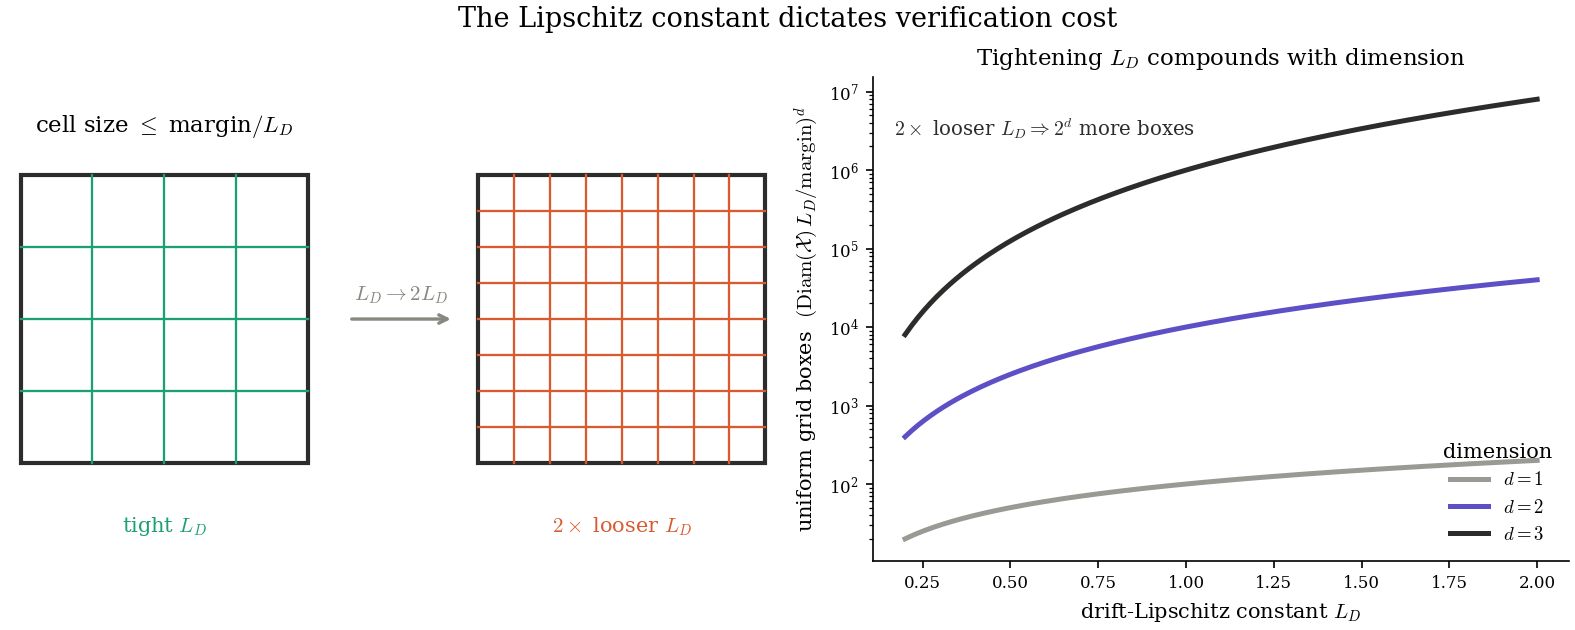
\includegraphics[width=0.92\linewidth]{Figures/lipschitz_gridding.png}
\caption{The Lipschitz constant dictates verification cost. \emph{Left:} each cell must be small
enough that the drift cannot cross the margin within it, so cell size $\lesssim\text{margin}/L$; a
looser constant forces a finer grid. \emph{Right:} the box count \eqref{eq:boxcount} grows as the
$d$-th power of $L$, so tightening the constant compounds with dimension.}
\label{fig:gridding}
\end{figure}

\subsection{The Margin Budget}
\label{subsec:budget}

Beyond forcing a finer grid, the Lipschitz constant caps the margin $\varepsilon$ one can certify at all. If $\cert$ is $L_\cert$-Lipschitz then $\expe_{x'}[|\cert(x)-\cert(x')|]\le L_\cert\,\expe_{x'}[\|x-x'\|]$, and a valid margin at $x$ obeys $\varepsilon(x) \le \cert(x)-\expe[\cert(x')]\le L_\cert\expe[\|x-x'\|]$; taking the binding (slowest-moving) state,
\begin{equation}
\label{eq:budget}
    \varepsilon \;\le\; L_\cert\,\inf_{x}\expe_{x'}[\|x-x'\|].
\end{equation}
This illustrates the maximally feasible decrease $\varepsilon$ that we can verify for the entire domain. The right-hand side is a property of the \emph{dynamics} (the smallest expected step), so the scale-free invariant is the ratio $\varepsilon/L_\cert$: a certificate cannot certify more decrease per unit of its own Lipschitz constant than the system actually moves. This highlights the dangers of using Lipschitz-constrained networks as certificates, as an $L_\cert$ that is too small will violate $\varepsilon / L_\cert \le \inf_{x}\expe_{x'}[\|x-x'\|]$, making the verification problem infeasible. Figure~\ref{fig:budget} illustrates this ``budget'' empirically; \cite{badings2025logRASM} attack the same tension from the certificate side, reparameterising it to lower its theoretical constant.

\begin{figure}[htbp]
\centering
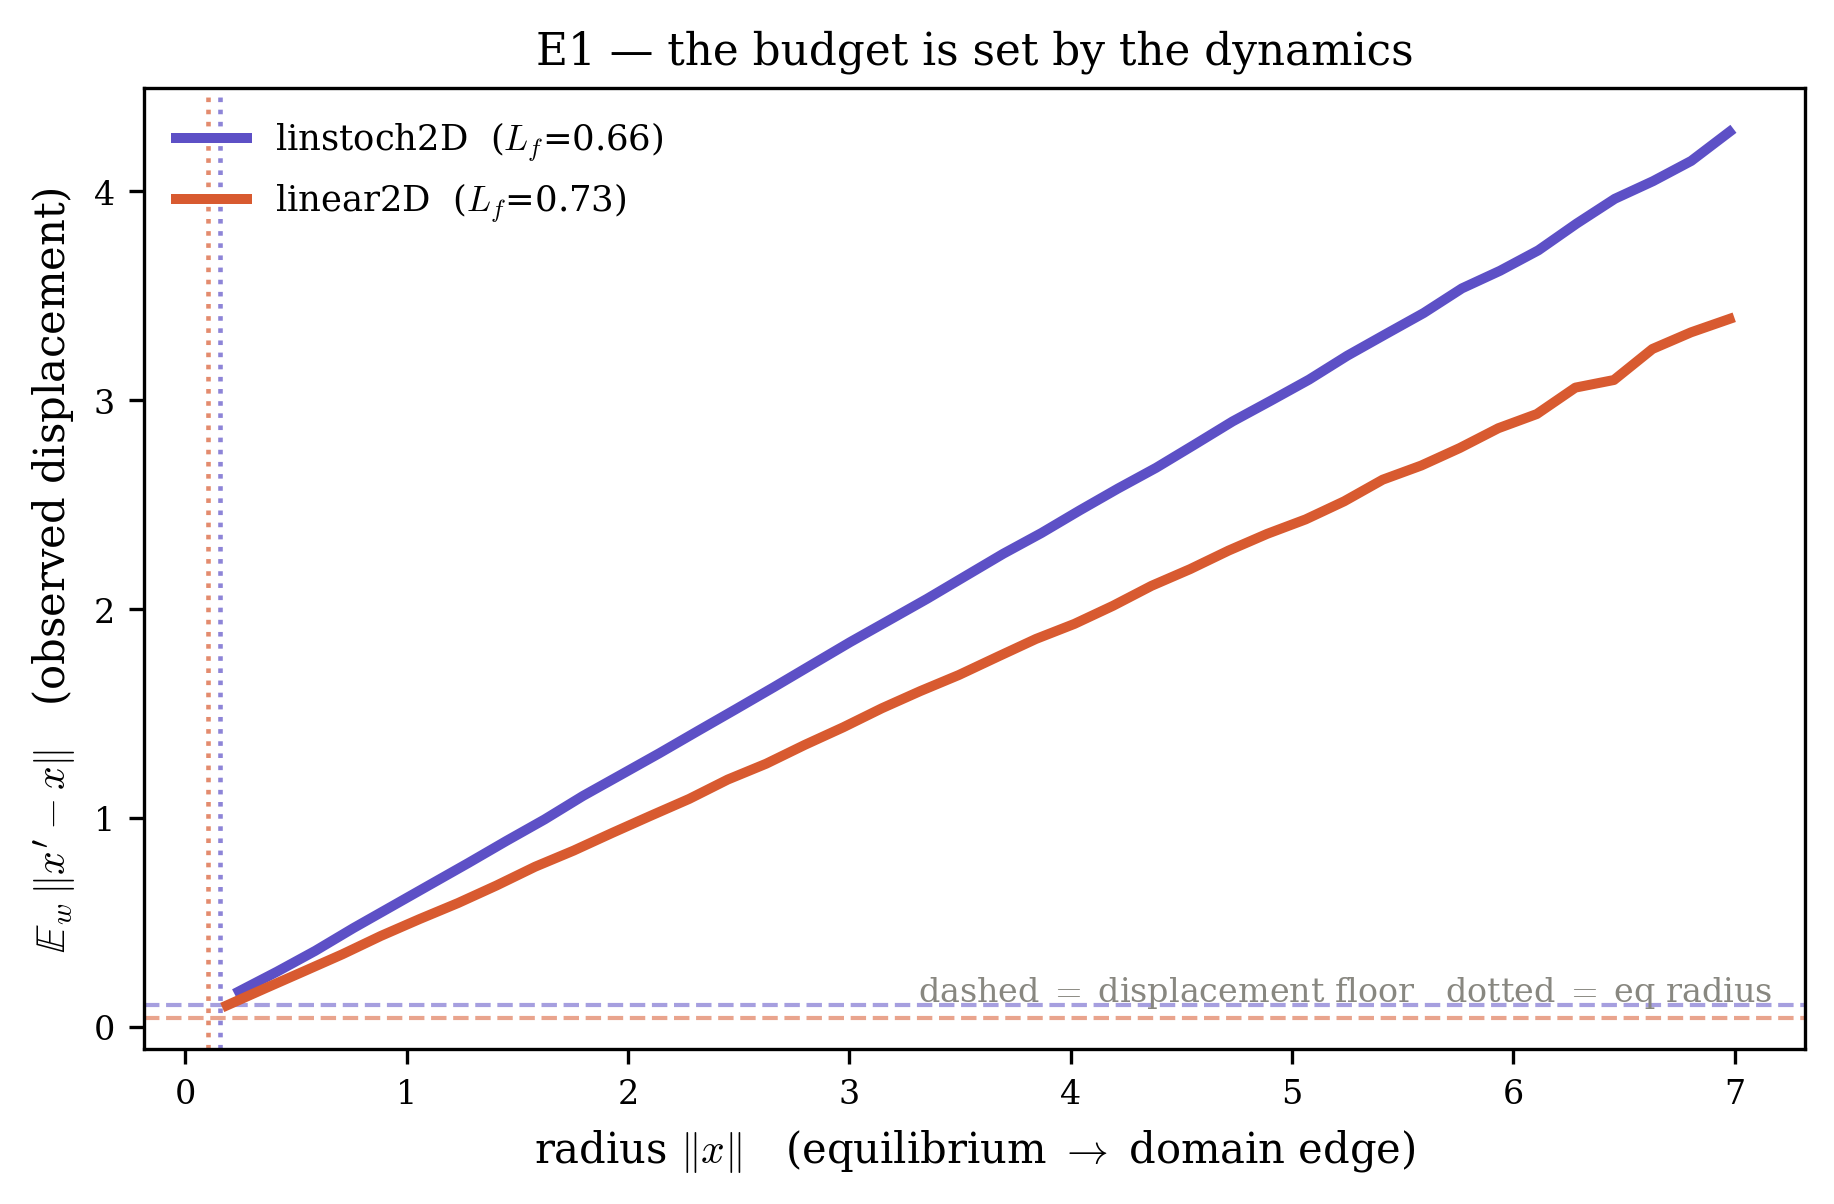
\includegraphics[width=0.64\linewidth]{Figures/lipschitz_budget_curve.png}
\caption{The budget \eqref{eq:budget} is set by the dynamics: the expected one-step displacement
$\expe_w\|x'-x\|$ rises from a floor near the equilibrium (which defines our domain-wide, fixed $\varepsilon$).}
\label{fig:budget}
\end{figure}


% ============================================================
\section{Tightening the Drift-Lipschitz Constant}
\label{sec:tightdrift}
% ============================================================

The sample-based verifiers in Section~\ref{sec:sampling-methods} consume one number: a sound upper bound on the drift-Lipschitz constant $L_\drift$. By \eqref{eq:boxcount} its magnitude drives an estimate on the cost to certify. To estimate $L_\drift$, one might derive a loose product bound $L_\drift \le L_\cert(L_f+1)$ via the composition bounds of \eqref{eq:lipschitz-composition} and Section~\ref{sec:nn_estimation}. However, we have established that composing global bounds is loose, assuming a worst-case alignment that inflates the discretisation error. We develop our tightenings in the deterministic setting of Section~\ref{subsec:gridding}, where the drift is $D$ \eqref{eq:det-drift} and the product bound reads $L_D \le L_\cert(L_f+1)$.

\subsection{Exact $L_D$ Computation}

For this contribution we assume that the dynamics $f$ are deterministic and linear, and $\cert$ is piecewise linear (for example a feed-forward $\mathrm{ReLU}$ network), with constant gradient $g_i$ on each activation region $R_i$. Given this, $\nabla D$ is piecewise constant.

\begin{proposition}[Exact drift-Lipschitz constant]
\label{prop:exactLD}
For linear $A$ and piecewise-linear $\cert$,
$\;L_D=\max\{\|A^\top g_j-g_i\| : R_i\cap A^{-1}R_j\cap\aX\neq\emptyset\}$.
\end{proposition}
\medskip\noindent\emph{Proof sketch.}\ $D$ is piecewise linear, so its Lipschitz constant is the maximum gradient norm over its linear pieces. Each piece is a nonempty cell $R_i\cap A^{-1}R_j\cap\aX$, on which $\nabla D=A^\top g_j-g_i$.\hfill$\square$\medskip

The exact constant improves on the product bound in two ways: it splits $\|A^\top g_j-g_i\|\le\|A\|\,L_\cert+L_\cert$ by the triangle inequality (the product bound discards the cancellation between the two terms), and it maximises over $i,j$ independently (the product bound discards that $x$ is the same point in both terms). Soundness of the estimate rests on a simple invariant: for any set $S$ containing every feasible pair, $\max_{(i,j)\in S}\|A^\top g_j-g_i\|\ge L_D$, so starting from all pairs and pruning only \emph{certifiably} infeasible ones can only tighten the bound, never break it. In practice we run LipBaB on the single network $D=\cert\circ A-\cert$; being anytime-sound, it returns a valid bound even on early termination.

\subsection{Results}

Table~\ref{tab:tightdrift} reports three sound upper bounds on $L_D$ for trained certificates on deterministic linear systems in $2$--$4$ dimensions ($\|A\|_\infty<1$, so the composition bounds are sound over the same box). M1 calculates $L_D$ by computing the product of spectral norms through the network (\eqref{eq:lipschitz-layer}) for $L_\cert$, which is then composed with $L_f$. M2 calculates $L_D$ in the same way, but uses LipBaB to compute the exact constant for $L_\cert$. Finally, M3 is the new proposition, where we use LipBaB to compute $L_D$ directly.

Running the branch-and-bound on the drift (M3) is consistently $1.3$--$1.5\times$ tighter than the best composition bound (M2) and $2.8$--$4.6\times$ tighter than the spectral product (M1). By \eqref{eq:boxcount} the M2$\to$M3 factor alone divides the box count by $(1.4)^d$, about $2\times$ in 2D and $3.8\times$ in 4D.

\begin{table}[htbp]
\centering
\begin{tabular}{cc rrr rr}
\hline
$d$ & $L_f$ & M1 spectral & M2 LipBaB & M3 drift & M1/M3 & M2/M3 \\
\hline
2 & 0.54 & 1.10 & 0.37 & 0.27 & $4.0\times$ & $1.4\times$ \\
2 & 0.60 & 1.60 & 0.52 & 0.38 & $4.3\times$ & $1.4\times$ \\
3 & 0.45 & 1.16 & 0.55 & 0.42 & $2.8\times$ & $1.3\times$ \\
4 & 0.55 & 1.78 & 0.92 & 0.60 & $2.9\times$ & $1.5\times$ \\
4 & 0.51 & 3.11 & 0.94 & 0.67 & $4.6\times$ & $1.4\times$ \\
\hline
\end{tabular}
\caption{Sound drift-Lipschitz estimates (upper bounds on $L_D$). M1 = product of spectral norms;
M2 = LipBaB on $\cert$ composed via $(L_f{+}1)$; M3 = LipBaB run on the drift $\cert\circ A-\cert$. M3 is uniformly
tightest.}
\label{tab:tightdrift}
\end{table}

\subsection{Anisotropic constants for free}
\label{subsec:aniso}


\paragraph{Directional constants.} Finally, a single global constant can be replaced by \emph{directional} ones. For a unit direction $v$, $L_f(v):=\sup_x\|J_f(x)\,v\|\le L$ is often far smaller, and for a scalar certificate it is one gradient projection to evaluate. We show that LipBaB yields these \emph{soundly}, and that they sharpen the verifier's discretisation.


LipBaB already computes, per leaf of its search, the exact per-region gradient; the per-axis constant $L_\cert(e_i)=\sup_x|\partial \cert/\partial x_i|$ is simply the component-wise maximum of those gradients over the (finitely many, fully enumerated) regions --- a \emph{sound} bound satisfying $L_\cert(e_i)\le L_\cert$. These anisotropic constants sharpen the discretisation: over an axis-aligned cell of side $w_i$ the sound bound $|\cert(x)-\cert(y)|\le\sum_i L_\cert(e_i)\,w_i$ replaces the isotropic $L_\cert\|w\|$, and refining each axis to its own sensitivity ($w_i\propto 1/L_\cert(e_i)$) reduces the box count from $\propto L_\cert^{\,d}$ to $\propto\prod_i L_\cert(e_i)$, a factor $\prod_i\big(L_\cert/L_\cert(e_i)\big)\ge 1$. We report the per-axis constants of the certificate; running LipBaB on the drift network $D=\cert\circ A-\cert$ (as in M3) yields the per-axis drift constants $L_D(e_i)$ by the identical extraction, and it is these that enter the box count \eqref{eq:boxcount}.

Table~\ref{tab:aniso} measures this on the same certificates. The per-axis constants are all below the global one and the reduction, being a product over axes, compounds with dimension: from $\approx1.5\times$ in 2D to $\approx8$--$17\times$ in 4D. Because it multiplies the M2$\to$M3 gain above, the two contributions stack.

\begin{table}[htbp]
\centering
\begin{tabular}{cc l r}
\hline
$d$ & $L_\cert$ (global) & per-axis $L_\cert(e_i)$ & box-count reduction \\
\hline
2 & 0.24 & $(0.22,\,0.18)$ & $1.5\times$ \\
2 & 0.32 & $(0.27,\,0.22)$ & $1.8\times$ \\
3 & 0.38 & $(0.36,\,0.20,\,0.18)$ & $4.1\times$ \\
4 & 0.60 & $(0.32,\,0.41,\,0.26,\,0.23)$ & $17.0\times$ \\
4 & 0.62 & $(0.41,\,0.46,\,0.40,\,0.26)$ & $7.8\times$ \\
\hline
\end{tabular}
\caption{Sound anisotropic (per-axis) Lipschitz constants extracted from LipBaB, and the resulting
axis-aligned box-count reduction $\prod_i(L_\cert/L_\cert(e_i))$. Every $L_\cert(e_i)\le L_\cert$; the saving
compounds with dimension.}
\label{tab:aniso}
\end{table}


% ============================================================
\section{Discussion}
% ============================================================

The two framings of this chapter are one picture. The Lipschitz constant is, to machine learning, a robustness quantity to estimate \cite{fazlyab2019lipsdp,bhowmick2021lipbab} and control \cite{miyato2018spectral,araujo2023unified}; to formal methods, the bridge that turns finite evidence into a whole-domain guarantee \cite{wu2020game,berkenkamp2017safe}. Certificate verification needs both at once, and because verification cost is a $d$-th power of the constant \eqref{eq:boxcount}, its magnitude is decisive. There are two levers: shrink the constant by controlling the architecture (Section~\ref{sec:control}), trading expressivity, or estimate it more tightly, changing nothing about the certificate but much about the cost of verifying it. Our two contributions take the second route on the exact object the verifiers consume --- the drift constant --- computing it directly rather than by composition, and extracting sound per-axis constants that sharpen the grid; because the two savings multiply, they reduce the box count by more than an order of magnitude in four dimensions. The core limitation is that both lean on the linearity that keeps the drift a $\mathrm{ReLU}$ network. Extending them to nonlinear dynamics, where the composed drift is no longer piecewise linear, is the clear next step, and would likely rely on another tool such as bound propagation.

\newpage

    % !TEX root = ../MasterThesis.tex
\normallinespacing

\chapter{Benchmarks}
\label{chap:benchmarks}

In this project we compare the strengths and weaknesses of a range of
certificate verification methods. The suite therefore spans a broad range of
system types, drawn from the literature to expose where each method succeeds and
fails. By identifying structural features of systems that make verification easy
or hard, we can separate each method along interpretable axes.

We select systems from the formal-methods and control literature so that the
suite spans three orthogonal axes of difficulty:

\begin{itemize}
  \item \textbf{Dynamics class.} From linear, through polynomial, to
        transcendental (e.g.\ trigonometric) dynamics. This axis directly controls
        which symbolic engines can encode the one-step map \emph{exactly}.
  \item \textbf{Noise model.} We assume that the noise distribution is bounded for each system.
        We include systems ranging from discrete to continuous additive noise variables,
        and from internal, state-dependent noise to external additive noise.
  \item \textbf{Dimension.} The linear families scale to arbitrary dimension,
        allowing us to explore how the curse of dimensionality affects each method.
\end{itemize}

A second selection principle is the \textbf{certificate class} each system
admits. Some systems have a known, analytic ground-truth certificate (a
quadratic $x^\top P x$, an $L_1$ piecewise-linear function, or a physical
potential), which lets us measure a verifier against a \emph{known-good} answer;
others have no closed-form certificate and the certificate must be learned,
exercising the full CEGIS loop.

Each benchmark instantiates the discrete-time stochastic system
\eqref{eq:stochastic-system}: its dynamics and noise model fix the transition
kernel $P(\cdot \mid x)$ of Section~\ref{subsec:kernels}, and with it the
one-step expectation inside the drift \eqref{eq:drift-def} that every verifier
of Chapter~\ref{chap:verification} must bound. The selection axes are therefore
precisely the levers that control how hard that expectation is to work with:
the dynamics class governs whether the one-step map can be encoded symbolically, the
noise model governs whether the expectation is an exact finite sum or must be
soundly over-approximated, and the dimension scales both.

\begin{table}[h]
\centering
\caption{The benchmark suite across the three selection axes.}
\label{tab:bench-suite}
\begin{tabular}{llll}
\hline
\textbf{System} & \textbf{Dynamics} & \textbf{Noise} & \textbf{Analytic Certificate} \\
\hline
$\mathrm{LinSwitch}$    & PWL / jump     & multiplicative (switch) & $L_1$ PWL (exact)  \\
$\mathrm{LinStoch}$   & linear         & additive bounded        & quadratic $x^\top P x$ \\
$\mathrm{DoubleWell}$        & polynomial     & additive bounded        & potential\\
$\mathrm{Pendulum}$     & transcendental & additive triangular     & none \\
\hline
\end{tabular}
\end{table}

Phase portraits of all four 2D systems (the expected drift field with sample
trajectories overlaid) are collected in Appendix~\ref{app:benchmark-portraits}.

% =====================================================================
\section{Linear Systems}
\label{sec:bench-linear}

% ---------------------------------------------------------------------
\subsection{$\mathrm{LinSwitch}$}
\label{sec:bench-switched}

The randomly switched linear system is a canonical model in the stochastic
stability literature, where at each step the dynamics matrix is selected by an
i.i.d.\ Bernoulli switch:
\[
  x_{t+1} = A_{\sigma_t} x_t, \qquad \sigma_t \sim \text{Bernoulli}(p).
\]
We instantiate the randomly switched systems framework of Chatterjee \&
Pal~\cite{chatterjee2009excursion}, who give conditions for almost-sure and
$L_1$ stability of such systems. Our 2D instance uses a pair of matrices chosen
to satisfy their contractivity conditions, being jointly contractive in the
$L_1$ norm. Randomly switched systems model phenomena such as mode-switching
control, packet loss over lossy channels, and Markov-jump linear dynamics. A
phase portrait of the 2D instance is given in Figure~\ref{fig:phase-linswitch}.

This is the \emph{simplest} stochastic obstruction in the suite and our
soundness baseline. The switch is an \emph{internal, discrete} source of
randomness, so it is encoded as a small set of exact finite branches rather than
an over-approximated continuous noise box, leaving no relaxation anywhere in the
pipeline. Every engine handles it, which makes it the control case against which
we measure. The $L_1$-contractivity gives an \emph{exact piecewise-linear}
ground-truth certificate $\cert(x) = |x_0| + |x_1|$, so the verification
conditions hold with \emph{zero relaxation gap} in both SMT and MILP, a property
no other system in the suite shares. The construction also generalises. A
random-construction variant draws two matrices at a target spectral norm $<1$ in
any dimension, for which $\cert(x) = \lVert x \rVert_2$ is valid, letting us
probe dimensional scaling.


% ---------------------------------------------------------------------
\subsection{$\mathrm{LinStoch}$}
\label{sec:bench-linstoch}

The additive-noise linear system,
\[
  x_{t+1} = A x_t + w_t, \qquad w_t \sim \text{bounded zero-mean noise},
\]
with $A$ Schur-stable, is \emph{the} canonical 2D example of the
stochastic-supermartingale literature~\cite{lechner2022stability, badings2025logRASM}. The deterministic part is
contractive, so the only obstruction to stability is the noise floor.
Figure~\ref{fig:phase-linstoch} shows the resulting inward spiral to the
noise-floor neighbourhood.

It is the additive-noise counterpart to the $\mathrm{LinSwitch}$ and isolates the
\emph{sound treatment of continuous additive noise}. The noise distribution is
over-approximated by a discretisation into cells so that the symbolic engines
soundly bound the expected drift. It is also the natural scaling testbed, since
$A$ can be constructed at any dimension and target spectral norm.

It admits an \emph{analytic} quadratic ground-truth certificate $\cert(x) = x^\top P
x$ with $P$ the solution of the discrete Lyapunov equation $A^\top P A - P = -Q$
($Q = I$). The expected drift then has the closed form
\[
  \expe[\cert(x')] - \cert(x) = -x^\top Q x + \operatorname{tr}(P\Sigma_w),
\]
which is $\le 0$ exactly outside a ball of radius
$r^\star = \sqrt{\operatorname{tr}(P\Sigma_w)/\lambda_{\min}(Q)}$. The
equilibrium radius is therefore \emph{derived from the noise level}, so $\cert$ is a
genuine supermartingale on $\text{domain}\setminus\text{equilibrium}$ (the
textbook ``a.s.\ stable to a neighbourhood'').


% ---------------------------------------------------------------------
\subsection{$\mathrm{DoubleWell}$}
\label{sec:bench-doublewell}

A 2D stochastic gradient-flow system on a tilted double-well potential,
\[
  x_{k+1} = x_k - \eta\,\nabla U(x_k) + w_k, \qquad
  U(x,y) = \tfrac14 (x^2 - 1)^2 + \tfrac12 y^2 - 0.3\,x .
\]
The double-well is the canonical model of metastability and noise-driven escape
over a potential barrier, originating with Kramers~\cite{kramers1940brownian} and
recurring throughout the Lyapunov-certificate literature as a bistable benchmark.
Figure~\ref{fig:phase-doublewell} shows the flow around the off-origin attractor.

It is the first \emph{nonlinear} (polynomial) system, while still
admitting an exact symbolic encoding (the cubic gradient is encoded via an
auxiliary squared variable in Z3/Gurobi). It tests whether a verifier handles a
non-convex value landscape and a non-origin equilibrium. The potential is
\emph{bistable}. The tilt $-0.3x$ breaks the symmetry so one well is the true
attractor, but the second (metastable) well is a basin the certificate must rule
out. The potential $U$ itself is the ground-truth Lyapunov function, giving an
interpretable, physically meaningful $\cert$. The equilibrium is off-origin (at
$\approx(1,0)$), unlike every other system.


\subsection{$\mathrm{Pendulum}$}
\label{sec:bench-pendulum-lqr}

The inverted pendulum is the archetypal control benchmark. We take the FOSSIL
\texttt{SineModel} pendulum with its verified LQR feedback gain $K = [[7.21,
1.34],[1.34, 0.33]]$~\cite{edwards2024fossil2, abate2021fossil},
folded into autonomous closed-loop dynamics, with additive triangular process
noise:
\[
  \theta' = \theta + h(\dot\theta + u_1), \qquad
  \dot\theta' = \dot\theta + h\!\left(u_2 + \tfrac{mgL\sin\theta - b\dot\theta}{mL^2}\right),
  \quad u = -Kx .
\]

This is the first \emph{transcendental} system. The $\sin\theta$ term means the
SMT and MILP engines cannot encode the map and must abstain, so only autoLiRPA
(which relaxes $\sin$) and the sampling/MAB engines apply. It also represents
dynamics found in the control literature, in which a controller returns actions
to influence a trajectory. Here $u$ is the controller and represents a torque
applied to the pendulum, and the equilibrium is its upright position, which would
otherwise be unstable if the controller was poor. The closed loop is Schur-stable but \emph{non-normal}
($\lVert A_d \rVert_2 > 1$, transient growth), so neither a box nor a ball is
forward invariant, and the domain is the Lyapunov sublevel ellipsoid of the
linearisation. Nonlinear dynamics and a controller add complexity beyond that of
the previous systems. Figure~\ref{fig:phase-pendulum} shows the closed-loop
spiral over the ellipsoidal domain.


\newpage

    % !TEX root = ../MasterThesis.tex
\chapter{Verification}
\label{chap:verification}

Verification asks whether the candidate certificate
$\cert$ satisfies the drift condition everywhere on the domain
(Definition~\ref{def:verification}). Each method answers this question in its own way, and the methods differ sharply in what they demand and what they return.
We group them into three families. \emph{Symbolic} methods encode the
certificate and the dynamics exactly and search for a violating assignment; they
need full white-box access and struggle with scaling. 
\emph{Abstract interpretation} propagates sound over-approximations of the
network through each layer; it requires a computation graph for the condition of interest. A spectrum of methods allows tuning between tightness and speed. \emph{Sampling}
methods evaluate the drift only at points, so they work for black-box
dynamics, at the cost of a probabilistic rather than exact guarantee.

\section{Symbolic Solvers}

With symbolic methods, the main challenge is encoding. We require full, white-box access in order to precisely encode each constraint. This includes full access to the underlying dynamic system, including any noise, and the candidate certificate.

Symbolic methods feature heavily in deterministic verification settings
\cite{katz2017reluplex, abate2020lyapunov, peruffo2020barrier, abate2021fossil}; supermartingales, however, require the encoding of an expected value. For discrete noise distributions this is manageable: one enumerates the outcomes and takes the weighted average. In many cases, however, the noise is continuous, and no finite formula represents its expectation exactly. In this case, we employ a common strategy of discretising the noise pdf and over-approximating it in order to soundly reason over it
~\cite{lechner2022stability, zikelic2023reachavoid}.


\subsection{SMT}

Satisfiability Modulo Theories (SMT) directly extends Boolean satisfiability (SAT), the problem of finding a truth assignment satisfying a propositional formula. By allowing variables to range over richer domains governed by background theories such as nonlinear real arithmetic, we seek to find a satisfying assignment. In our context, we look for an assignment satisfying the negation of the supermartingale condition; it is this assignment that forms a counterexample.
\[
\exists x \in \aX : \drift(x) > 0
\]

We use Z3 as our SMT backend
\cite{demoura2008z3}. The ReLU certificate is piecewise-linear, so it
encodes exactly: each neuron becomes a case split, and the expected value in the
drift is a weighted sum over the noise branches. Z3 reasons in exact arithmetic
\cite{jovanovic2012nlsat},
so when it returns a verdict there is no numerical slack to worry about.

Z3's nonlinear real arithmetic is a sound and complete decision
procedure for polynomial constraints, so quadratic and even cubic dynamics such
as those in $\mathrm{DoubleWell}$ are handled exactly. The main difficulty lies in scalability.
Even on minimal problems (such as a tiny trained network of two layers of four neurons), Z3 frequently returns \emph{unknown} or exhausts its time budget (3600s).

Compounding this, continuous noise cannot be represented exactly, but it can be soundly over-approximated by binning it into a finite set
of branches with a conservative encoding whose slack shrinks as the number of bins
grows. This also grows the number of variables that Z3 must check, worsening the scalability wall above.

In addition, Z3 cannot handle transcendental relationships, which restricts both the dynamics we can certify ($\mathrm{Pendulum}$ system requires $\sin(x)$) and the certificates we can check (no sigmoid or tanh network architecture). Tools built on $\delta$-complete decision procedures, such as dReal
\cite{gao2013dreal}, can reason over these transcendental functions, but only up to a user-specified numerical error rather than exactly.

\subsection{MILP}

Mixed Integer Linear Programming (MILP) extends beyond satisfiability to optimisation problems. By combining propositions and numerical constraints, we represent the verification problem as maximising the drift $\drift$ (see Chapter~\ref{chap:refutation} for more details on defining optimisation problems), and if there exists a solution greater than 0, we reject the candidate.

We use Gurobi (version 13.0.1, via \texttt{gurobipy}) as our MILP backend
\cite{gurobi2026manual}. Casting verification as an optimisation
rather than a satisfiability query has a practical benefit: the solver returns
the worst-case drift as a number, so we learn not just \emph{whether} the
certificate fails but by how much. The $\relu$ certificate encodes with the usual
indicator and max constraints.

As with SMT, polynomial dynamics remain within reach, even though the tool is designed for piecewise-linear problems.

Enabling Gurobi's nonconvex mode turns it into a spatial branch-and-bound solver: it encloses each
product term in a convex relaxation and refines the variable ranges until the
relaxation is tight, converging to the global optimum. This is what lets it
verify the cubic $\mathrm{DoubleWell}$ exactly. One caveat
unique to Gurobi is that it works in floating point, so its guarantee holds only up
to the solver's numerical tolerances. Otherwise, the model grows with the network width and
the number of noise bins, echoing the scalability issues of SMT. As before, transcendental dynamics remain out of scope. Noise is handled exactly as in the SMT case: discrete outcomes enumerated,
continuous noise binned into a sound over-approximation.

The number of bins used to discretise the noise distribution is the crux of the
method's behaviour on stochastic dynamics. Writing $b$ for the
bins per noise dimension and $d_w$ for the dimension of the noise variable $w$, the expectation $\expectation$ is over-approximated
by $b^{d_w}$ cells, each carrying its own copy of the successor-network encoding,
so the program grows as $b^{d_w}$ (Figure~\ref{fig:milp_size}). With too few bins the over-approximation is so loose
that its drift exceeds the threshold even for a valid certificate: the
maximiser returns \emph{phantom} counterexamples --- a state whose true expected
drift is negative but whose binned over-approximation is positive --- and the CEGIS
loop is sent chasing a violation that does not exist. With too many bins the $b^{d_w}$
network copies make the program so large that the solver can no longer close the
optimality gap within the time budget. Only an intermediate \emph{window}
of $b$ both tightens the over-approximation enough to certify and stays small enough to
solve.


\begin{figure}[t]
  \centering
  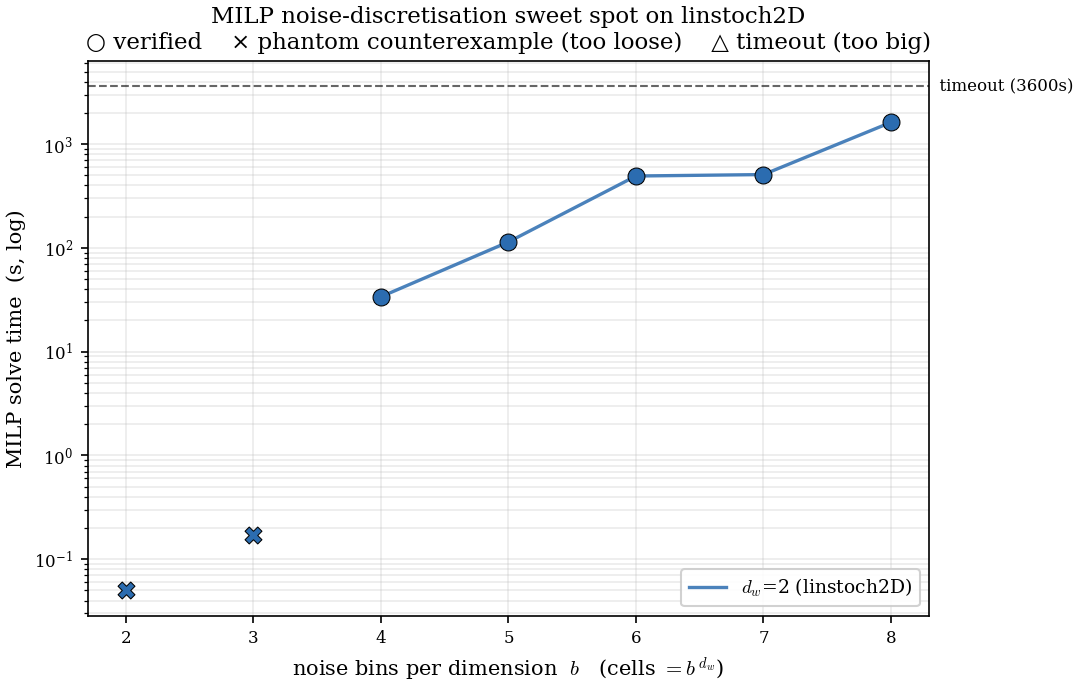
\includegraphics[width=0.85\textwidth]{Figures/milp_noise_disc.png}
  \caption{MILP verification of a stochastic-linear certificate on the
    two-dimensional $\mathrm{LinStoch}$ system, against the noise discretisation
    $b$ (bins per noise dimension, so the model carries $b^{d_w}$ noise cells).
    The \emph{phantom} regime below $b = 4$ and the steep growth in solve time
    above it (the cell count itself grows as $b^{2}$) are discussed in the text.}
  \label{fig:milp_nd}
\end{figure}

\begin{figure}[t]
  \centering
  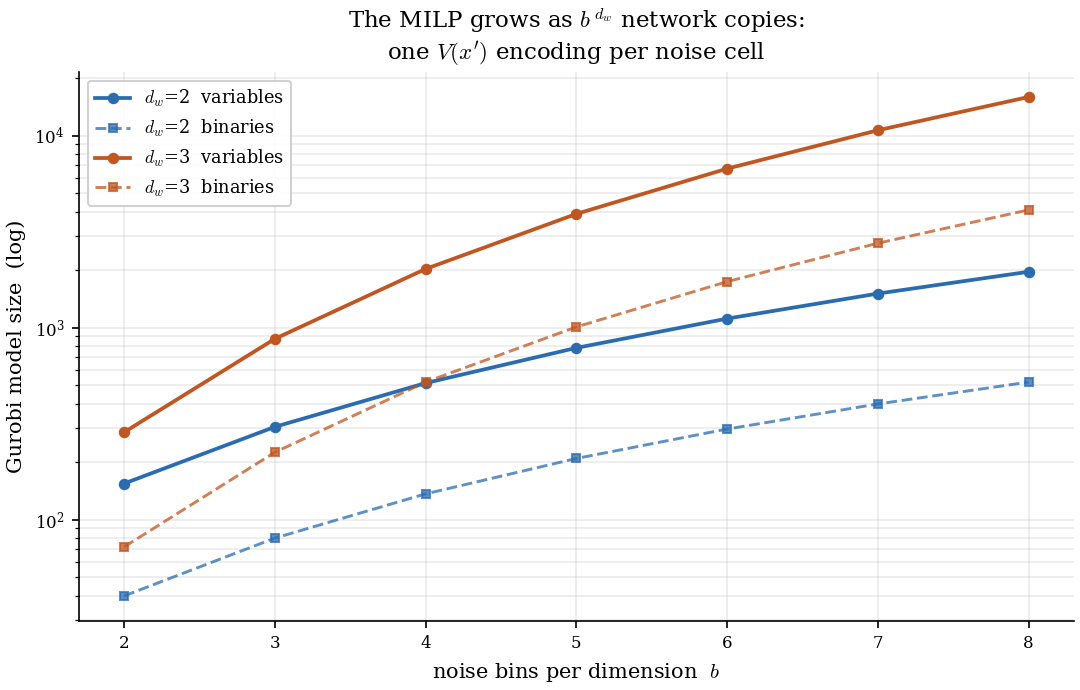
\includegraphics[width=0.7\textwidth]{Figures/milp_problem_size.png}
  \caption{The Gurobi model size (decision variables and
    binaries) grows as $b^{d_w}$, since each of the $b^{d_w}$ noise cells must represent and optimise over its
    own copy of the successor-network encoding. Tightening the
    over-approximation (larger $b$) and staying solvable are therefore in direct
    conflict, and the conflict is exponential in the noise dimension $d_w$.}
  \label{fig:milp_size}
\end{figure}

Figure~\ref{fig:milp_nd} traces this behaviour on $\mathrm{LinStoch}$ in two
dimensions. Below $b = 4$ the over-approximation is so loose that every candidate is
rejected by a phantom counterexample; from $b = 4$ onward the certificate verifies.
The cell count grows as $b^{2}$, and the solve time climbs far faster still, from $34$\,s
at $b = 4$ to some $27$ minutes at $b = 8$. No bin count in the swept range exhausts
the one-hour budget, so in two dimensions the binding constraint is the phantom
threshold below, not a timeout above.

The window nonetheless closes with dimension. Because the cell count is $b^{d_w}$, the
same sweep in three noise dimensions never escapes the phantom regime: every bin count we
could solve, up to $b = 8$ ($512$ cells), still returns a phantom counterexample,
while the $b^{3}$ growth drives a single solve past $1600$\,s by $b = 7$. No bin count
is at once tight enough to certify and cheap enough to solve, so the exact route
stalls without ever producing a valid certificate. This places the exact route's limit
between two and three noise dimensions, consistent with the frontier the
stochastic-certificate literature places at a handful of
dimensions~\cite{badings2025logRASM, lechner2022stability}.



\section{Abstract Interpretation}
\label{sec: abstract-interpret}

Rather than encode the problem exactly, abstract interpretation
over-approximates it. Given an input region, we propagate \emph{bounds} through a computation graph, so that the true output is always guaranteed
to lie within the computed enclosure. This makes the method sound by
construction: if the enclosure of the drift stays below the threshold, no input
in the region can violate it. The price is looseness (the enclosure is wider
than the true reachable set), and the central trade-off is how much tightness we
are willing to pay for. % CITED-QUOTE (xu2020autolirpa): "by generalizing existing LiRPA algorithms such as CROWN to operate on general computational graphs."
We use the auto\_LiRPA framework \cite{xu2020autolirpa}, which spans this
spectrum from cheap interval bounds to tighter linear relaxations.


\subsection{Interval Propagation}

Interval bound propagation
\cite{gowal2018ibp} is the simplest instance: we carry an interval
$[\underline{z},\overline{z}]$ for each neuron and push it through the affine and
activation layers. It is cheap and unconditionally sound, but also the loosest
option. Because it tracks each neuron independently, it ignores the correlations
between them: every $\relu$ that straddles zero is relaxed in isolation, so the
intervals widen quickly with depth and width. On our trained certificates the
enclosure is usually too loose to verify without extensive splitting of the input
region.


\subsection{Linear Relaxation}

CROWN \cite{zhang2018crown} tightens this by propagating \emph{linear} bounds rather than intervals:
each neuron is bounded above and below by an affine function of the inputs, which
preserves the inter-neuron correlations (unlike IBP) and yields far
tighter enclosures at a moderate cost. Where a single pass is still too loose to
decide a region, we close the gap with branch-and-bound, splitting the region and
bounding each piece. Optimising the relaxation slopes of each neuron by gradient
ascent --- \emph{$\alpha$-CROWN} \cite{xu2021alphacrown} --- yields a still-tighter
bound at a higher per-call cost, and is the strongest of the three engines we use.
One practical wrinkle is that the bound-propagation library
only supports a fixed catalogue of operations, so a certificate's output
activation must be expressed in terms it recognises: our hard-sigmoid activation function, for
instance, is decomposed into a scaling and a clamp. Figure~\ref{fig:box-evolution}
shows this branch-and-bound partition evolving on the $\mathrm{Pendulum}$
certificate, each cell shaded by whether its sound enclosure has yet cleared the
threshold.

\begin{figure}[htbp]
\centering
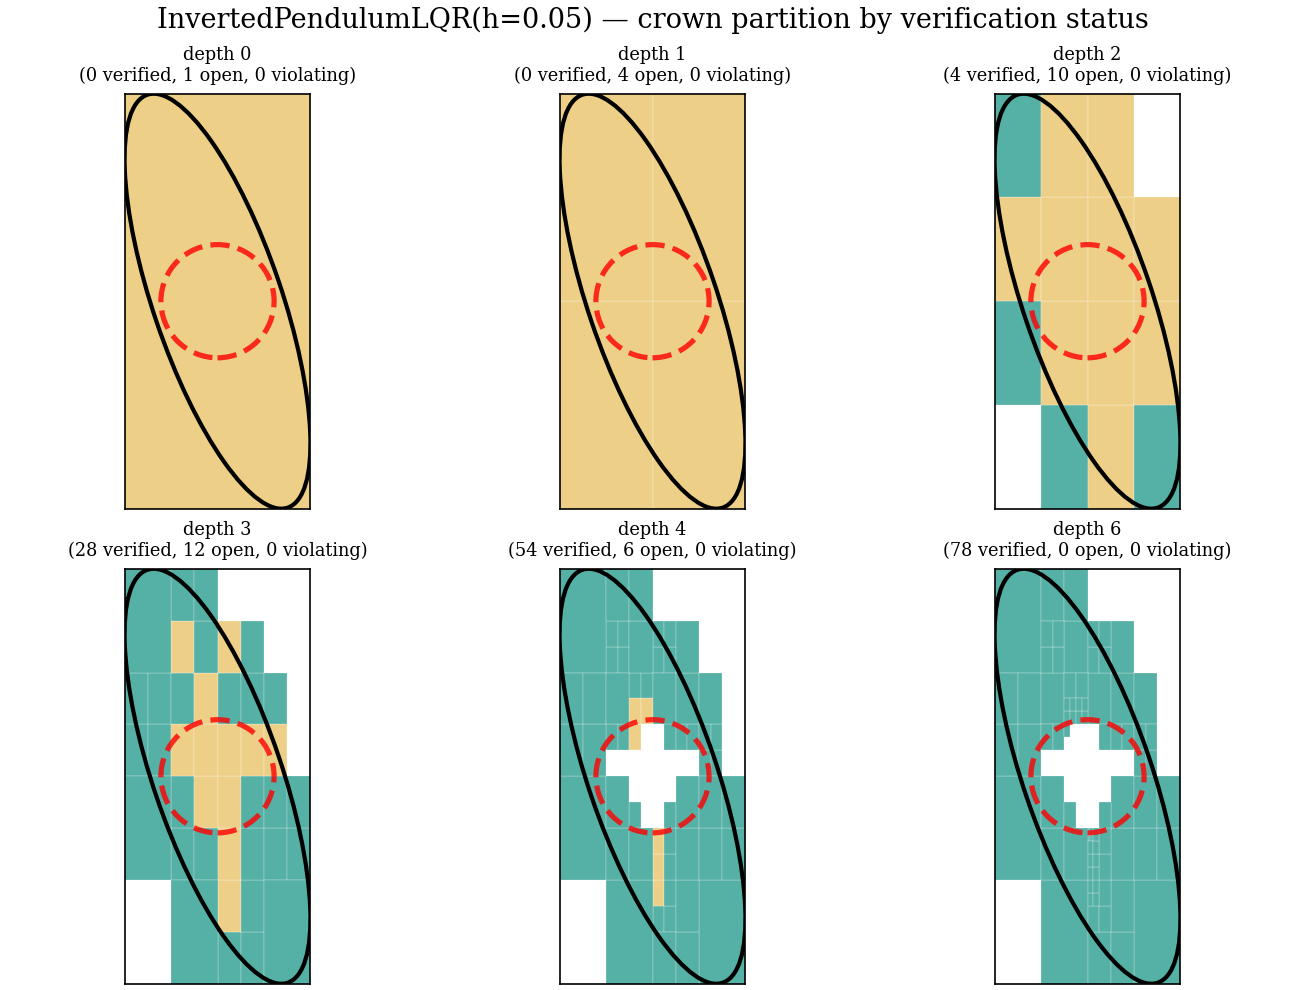
\includegraphics[width=0.85\linewidth]{Figures/pendulum_lqr_crown_grid.png}
\caption{Branch-and-bound in action: CROWN's partition of the 2D $\mathrm{Pendulum}$
state space at successive depths, for a verified certificate. Each cell is shaded by
its sound status --- \emph{verified} (drift upper bound $\le 0$, teal),
\emph{undecided} (amber, still to be split), or \emph{violating} (red); the black
curve marks the domain boundary and the red dashed circle the goal region. From a
single undecided box, auto\_LiRPA repeatedly halves the cells it cannot yet decide
until the whole domain is verified. Tighter relaxations reach this state with far
fewer splits than IBP --- the compute that the anytime view of
Figure~\ref{fig:pendulum-anytime} prices.}
\label{fig:box-evolution}
\end{figure}

CROWN tools such as \texttt{jax\_verify} \cite{jax_verify} and auto\_LiRPA require noise to be over-approximated through binning, as with the symbolic methods. Furthermore, they are not natively designed to handle discrete noise, requiring the spawning of multiple separate process threads to evaluate.


\begin{figure}[htbp]
\centering
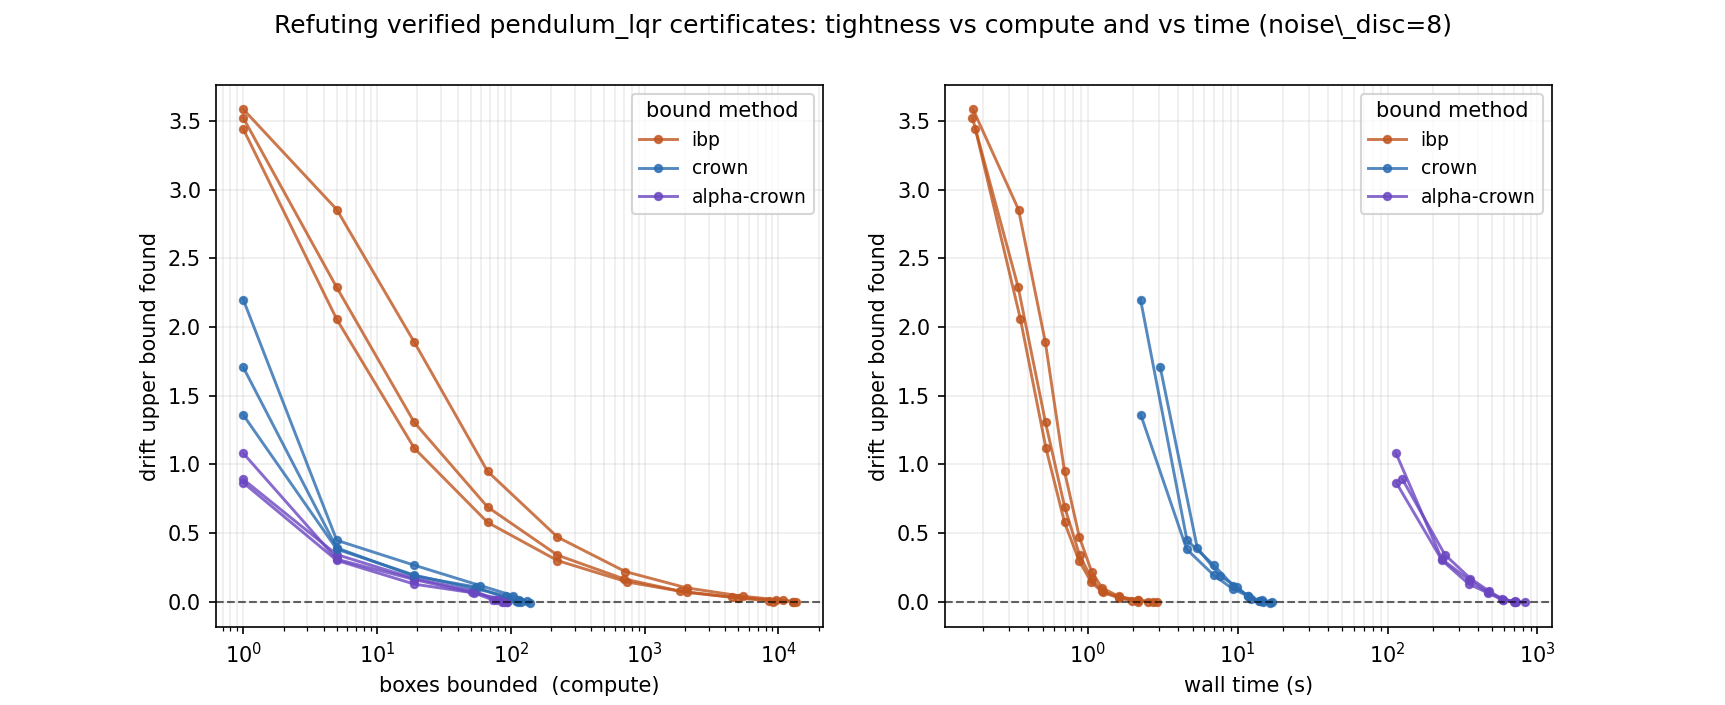
\includegraphics[width=0.82\linewidth]{Figures/pendulum_anytime.png}
\caption{Anytime tightness of the three bound-propagation engines on a verified
$\mathrm{Pendulum}$ certificate: the sound drift upper bound against wall-clock as
branch-and-bound refines. IBP is cheapest per unit compute but loosest, requiring the most domain partitions;
$\alpha$-CROWN reaches the tightest bound at the highest cost; CROWN sits between.
All three are sound at every step, as the bound only tightens.}
\label{fig:pendulum-anytime}
\end{figure}

\paragraph{Anytime Tightness.} Every engine in this family only ever \emph{tightens} its sound bound as
branch-and-bound refines, so it can be halted at any point and still return a
valid enclosure --- an \emph{anytime} guarantee that the drift $\drift$ exceeds the current upper bound nowhere. In particular, tighter bounding means less branching is required, and so fewer domain regions to check. Figure~\ref{fig:pendulum-anytime}
makes the resulting speed--tightness trade concrete on a verified
$\mathrm{Pendulum}$ certificate: IBP is the loosest at any compute budget, CROWN
tightens it, and $\alpha$-CROWN reaches the tightest bound at the highest cost.
This anytime soundness is precisely the property the CEGIS loop of
Chapter~\ref{chap:streamlining} exploits, since a verifier call can be stopped the
moment its bound crosses zero.





\section{Sampling}
\label{sec:sampling-methods}

Sampling methods sit at the opposite extreme from symbolic ones~\cite{zikelic2023reachavoid}.
They are the easiest to implement, since they need only sample
access to $\drift$: any form of noise or dynamics can be sampled without ever
representing its structure, and that flexibility is the whole appeal. The difficulty lies in providing a rigorous guarantee from finitely many points; an average over a
finite set of points says nothing about the gaps between them. What makes these
methods sound is a \emph{regularity} bridge, the drift-Lipschitz constant $L_\drift$, which
bounds how much the drift can change between samples; and even then the guarantee
is \emph{probabilistic}, holding with a chosen confidence $1-\delta$. For deeper discussion on estimating the Lipschitz constant, see Chapter~\ref{sec:lipschitz}. We discuss two methods below, a global Monte Carlo
estimate and an adaptive multi-armed-bandit search.

A sampling verifier evaluates $\drift$ only at finitely many points, so the
whole difficulty is bridging soundly from those points to the continuum between
them. Both methods below do so with a rigorous \emph{drift-Lipschitz} constant
$L_{\drift}$; as shown in Chapter~\ref{sec:lipschitz}, a valid choice is
$L_{\drift} = L_{\cert}\,(L_f+1)$, where we assume knowledge of a sound one-step Lipschitz constant of the dynamics $L_f$, and $L_{\cert}$ is a bound on the certificate's Lipschitz constant.

Each method relies on a simple concept: the confidence bound for a grid cell $B \in \mathcal{B}$ is derived from a statistical error as well as a discretisation error. The discretisation error is defined as the product of the diameter of $B$ and $L_\drift$, as we have seen before. The statistical error relies on Hoeffding bounds to estimate the confidence that the observed mean of the samples in $B$ reflects the true mean. This requires normalisation with respect to the range of values that $\drift$ can assume, which is non-trivial. To combat this, we restrict the class of $\cert_\theta$ that we can learn by constricting the output with either a clamp or a sigmoid activation. In our experiments, we clamp values in $[0,1]$ to avoid this normalisation step.

\subsection{Monte Carlo}
\label{sec:mc}

The Monte Carlo method is heavily inspired by the results and methods discussed in Chapter~\ref{sec:lipschitz}. We first discretise the domain uniformly according to $L_\drift$, and then take samples within each grid cell. We track the observed empirical mean of the drift on each cell $B$ and its statistical error to produce upper and lower confidence bounds. If the lower confidence bound for some $B$ is greater than zero, then we certifiably have a counterexample inside $B$. We return $B$ as a certified violating region and sample within it to supply the learner's next counterexamples. If the upper confidence bound is below zero, then we can certify that our certificate condition holds on $B$ with confidence $1-\delta$. If the process stalls, the discretisation error needs refinement, which motivates our next method.


% \paragraph{Underlying theory.}
% The natural sampling estimate of \eqref{eq:drift} is the \emph{average}
% exceedance $\mu = \expe_{X\sim\mathrm{Unif}(\aX)}[\max(0,\drift(X))]$,
% which a Hoeffding bound controls from finitely many draws. On its own this is
% \emph{unsound} as a verifier: the supremum we must bound is not controlled by
% the mean, because an arbitrarily thin violating spike contributes almost nothing
% to the average. Regularity is what closes the gap. If $\drift$ is $L_{\drift}$-Lipschitz a
% violation cannot be a spike: a point $x^\star$ with $\drift(x^\star)=\eta>0$ forces
% $\drift \ge \eta/2$ throughout the ball $\mathcal{B}(x^\star,\eta/2L_{\drift})$, so a large
% worst case necessarily inflates the average. This gives a quantitative exchange
% rate between the mean and the maximum.

% \begin{lemma}[Lipschitz mean-to-max]
% \label{lem:mc}
% Let $\drift$ be $L_{\drift}$-Lipschitz on $\aX\subset\RN^d$ and let
% $\mu = \expe_{X\sim\mathrm{Unif}(\aX)}[\max(0,\drift(X))]$. Then
% \begin{equation*}
%     \sup_{x\in\aX} \drift(x) \;\le\; \Phi(\mu),
%     \qquad
%     \Phi(\mu) := \Big(
%         \frac{2^{\,d+1}\, L_{\drift}^{\,d}\, \mathrm{Vol}(\aX)}{\kappa\, V_d}\, \mu
%     \Big)^{1/(d+1)},
% \end{equation*}
% where $V_d$ is the volume of the unit $d$-ball and $\kappa$ lower-bounds the
% fraction of a violation ball that lies inside $\aX$.
% \end{lemma}
% \medskip
% \noindent\textit{Proof sketch.}
% If $\eta:=\sup_x \drift(x)>0$ then $\drift\ge\eta/2$ on
% $\mathcal{B}(x^\star,\eta/2L_{\drift})\cap\aX$, whose volume is at least
% $\kappa\,V_d\,(\eta/2L_{\drift})^d$. Since $\max(0,\drift)\ge\eta/2$ there,
% $\mu \ge \tfrac{\kappa V_d}{2^{d+1}L_{\drift}^d\,\mathrm{Vol}(\aX)}\,\eta^{d+1}$;
% inverting for $\eta$ yields the bound.\hfill$\square$
% \medskip

% \paragraph{How it works.}
% The method is deliberately non-adaptive. It draws $n$ points uniformly from the
% working region, estimates the drift at each with $m$ successor samples of the
% inner expectation, and averages the exceedances to obtain $\widehat\mu$. A
% one-sided Hoeffding radius $r$ turns this into an upper confidence bound
% $\mu_{\mathrm{UB}} = \widehat\mu + r$ on the true mean $\mu$, valid with
% probability $1-\delta$. Lemma~\ref{lem:mc} then converts $\mu_{\mathrm{UB}}$ into
% a certified ceiling $\Phi(\mu_{\mathrm{UB}})$ on the worst-case drift. The nested
% inner estimate is harmless: $\max(0,\cdot)$ is convex, so by Jensen's inequality
% the noisy estimate over-shoots the true exceedance in expectation --- the safe
% direction for an upper bound. Finally, to look for a genuine counterexample the
% worst sampled point is re-evaluated with a large fresh batch of successor draws;
% only if its one-sided \emph{lower} confidence bound is positive is a violation
% reported, which prevents the maximum of many noisy estimates from being mistaken
% for a real one.

% \begin{algorithm}[H]
% \DontPrintSemicolon
% \KwIn{certificate $\cert$, dynamics sampler $f$, region $\aX$, margin
%   $\varepsilon$, confidence $\delta$, states $n$, inner draws $m$, drift-Lipschitz
%   $L_{\drift}$, value range $b$ (so $\cert\in[0,b]$), tolerance $\tau$}
% \KwOut{\textsc{Verified} / \textsc{Counterexample} / \textsc{Inconclusive}, and
%   a certified ceiling on $\sup_x \drift(x)$}
% $\kappa \leftarrow 2^{-d}$;\quad
% $\mathrm{Vol} \leftarrow$ volume of the bounding box of $\aX$;\quad
% $V_d \leftarrow \pi^{d/2}/\Gamma(\tfrac d2+1)$\;
% draw $x_1,\dots,x_n \sim \mathrm{Unif}(\aX)$\;
% \For{$i = 1,\dots,n$}{
%   $\widehat{\drift}_i \leftarrow \tfrac1m \sum_{j=1}^m \big[\cert(f(x_i,w_j)) - \cert(x_i) + \varepsilon\big]$
%   \tcp*{inner Monte Carlo}
% }
% $\widehat\mu \leftarrow \tfrac1n \sum_i \max(0,\widehat{\drift}_i)$;\quad
% $r \leftarrow (b+\varepsilon)\sqrt{\ln(1/\delta)/(2n)}$;\quad
% $\mu_{\mathrm{UB}} \leftarrow \widehat\mu + r$\;
% $\Phi \leftarrow \big(2^{d+1} L_{\drift}^{d}\,\mathrm{Vol}/(\kappa V_d)\cdot \mu_{\mathrm{UB}}\big)^{1/(d+1)}$
% \tcp*{Lemma~\ref{lem:mc}}
% $x^\star \leftarrow \arg\max_i \widehat{\drift}_i$;\quad re-estimate $\drift(x^\star)$ with a
% large fresh batch $\to$ lower bound $\ell$\;
% \lIf{$\ell > 0$}{\Return \textsc{Counterexample} $x^\star$}
% \lElseIf{$\Phi \le \tau$}{\Return \textsc{Verified} ($\sup_x \drift \le \tau$)}
% \lElse{\Return \textsc{Inconclusive} (ceiling $\Phi$)}
% \caption{Monte Carlo verifier (global Lipschitz mean-to-max)}
% \label{alg:mc}
% \end{algorithm}

% \paragraph{Requirements, strengths and limitations.}
% The method needs only \emph{sample} access to the dynamics --- it never encodes
% $f$ or $\cert$ --- together with a rigorous drift-Lipschitz bound $L_{\drift}$, a value
% range $b$ so that the exceedance is bounded, and the domain volume. Its strengths
% follow from that minimal interface: it is oblivious to the form of the noise and
% the dynamics, so continuous, discrete and transcendental systems are handled
% identically; it is embarrassingly parallel; and it is trivial to implement. Its
% weakness is the conversion in Lemma~\ref{lem:mc}. Reconstructing a
% $d$-dimensional volume back into a height costs the exponent $1/(d+1)$: with a
% Hoeffding radius $r\propto n^{-1/2}$ the certified ceiling shrinks only as
% $\Phi \propto n^{-1/(2(d+1))}$, so driving it below a tolerance $\tau$ requires on
% the order of $\tau^{-2(d+1)}$ samples. Crucially $\Phi(\mu_{\mathrm{UB}})$ is
% strictly positive for any finite budget (even with no sampled violation,
% $\mu_{\mathrm{UB}}$ equals the concentration radius), so the method can certify
% $\sup_x \drift \le \tau$ only for a \emph{positive} $\tau$ --- never $\sup_x \drift\le 0$
% outright.

% \paragraph{What it yields.}
% Algorithm~\ref{alg:mc} produces, with probability $1-\delta$, a sound numerical
% \emph{upper bound} on the worst-case drift over the entire region: a certified
% ceiling, not a binary verdict. It also returns genuine (re-confirmed)
% counterexamples when the certificate is violated. What it does \emph{not} give is
% a violating region --- the estimate is purely pointwise --- nor an exact proof.
% It is therefore best read as the sound-but-expensive baseline whose
% $\tau^{-2(d+1)}$ cost, and its inability to reach a zero tolerance, precisely
% motivate the adaptive method that follows.

\subsection{Multi-Armed Bandit}
\label{sec:mab}

We consider the Monte Carlo method to be non-adaptive: it samples uniformly in each grid cell, and the cells are uniformly sized. The Multi-Armed Bandit method seeks to improve on this through adaptive sampling and discretisation. We first consider the domain in its entirety and estimate its upper and lower confidence bounds on the mean drift. Similar termination rules apply; however, in the case where the confidence bound straddles zero (making our cell undecided), we consult the error bounds. If the discretisation error is greater than the statistical error, then we split the grid according to some fixed splitting rule. If the reverse is true, then we take more samples. With this, grid refinement is data-driven: grid cells with strong average decrease are verified early and can be pruned as potential violation locations.

Motivated by sample efficiency, in the case where multiple cells are undecided, we can check the top $k$ cells with the highest upper confidence bounds to act upon. With $k=1$, we take only the most unsure cell, where further sampling will be most beneficial. With larger $k$, we act upon more and more cells at once, approaching a more uniform gridding. We therefore see a tradeoff between sample-efficiency and time-efficiency through the parameter $k$.

\paragraph{Experimentation.} This method requires both tight estimation of $L_\drift$ and tight bounds on the statistical error. For our experiments, we used LipBaB (M2 in Section~\ref{sec:tightdrift}) and an empirical-Bernstein radius for the error bounding. Unfortunately, with loose bounds, we were unable to achieve termination within our sample budget ($10^9$ samples) for either method consistently on any benchmark.

\section{The Capability Boundary}
\label{sec:capability}

Across the suite the three families separate cleanly, and the boundary follows
the dynamics class and the noise dimension. The \emph{symbolic} engines are the
most precise where they apply but the least available: Z3, though a complete
decision procedure for the polynomial systems, returned \emph{unknown} or
exhausted its budget on essentially every trained-network round, and Gurobi's
exact route closes between two and three noise dimensions as the
discretisation window shuts (Figure~\ref{fig:milp_nd}); neither can encode the
$\mathrm{Pendulum}$'s transcendental dynamics, and both abstain there. The
\emph{sampling} verifiers are the most general in principle, indifferent to
the form of the noise and the dynamics, but sound worst-case sampling proved
too expensive in practice: within our budgets neither Monte Carlo nor the
multi-armed bandit could be driven to termination, so we do not carry them
forward as benchmarked engines. The \emph{bound-propagation} family has the
widest coverage and is the only one to reach the transcendental
$\mathrm{Pendulum}$ --- yet it is not universal either: $\mathrm{LinStoch}$,
whose noise-floor equilibrium leaves the relaxation little margin to work
with, was certified only by the exact MILP route inside its discretisation
window (Figure~\ref{fig:milp_nd}). No single family clears the whole suite;
the boundary is two-sided, with the exact route alone owning the additive-noise
linear system and bound propagation alone reaching past the symbolic frontier.
Within the LiRPA family, IBP, CROWN and $\alpha$-CROWN trade per-call
tightness against cost along the anytime curve of
Figure~\ref{fig:pendulum-anytime}.

This boundary fixes the cast for the remainder of the thesis. The three LiRPA
engines are the sound verifiers of the end-to-end synthesis campaign of
Chapter~\ref{chap:streamlining}, run on the three systems they certify, where their per-call costs (from
sub-second for IBP on $\mathrm{LinSwitch}$ to some twenty minutes for
$\alpha$-CROWN on the $\mathrm{Pendulum}$) are measured inside the loop.
And every round in which a verifier (MILP or LiRPA) rejected a candidate
leaves behind a genuine refutation problem; these rejected candidates form the
faux-certificate library on which Chapter~\ref{chap:refutation} benchmarks the
refuters. What no engine changes is the fundamental expense of a sound call,
which must reason over the entire domain; removing that cost from every round
of synthesis is the subject of the final chapter.

% \paragraph{Underlying theory.}
% The Monte Carlo verifier is \emph{global}: it reconstructs the worst case from a
% single average over the whole region, and Lemma~\ref{lem:mc} shows the price is a
% conversion no finite budget can drive to zero. The multi-armed-bandit (MAB)
% verifier removes that penalty by keeping the estimate \emph{local}. The region is
% covered by axis-aligned cells; on each cell $C$ we maintain a confidence interval
% on $\sup_{x\in C} \drift(x)$ that combines a statistical term, from the samples drawn
% in $C$, with a discretisation term, the cell diameter scaled by the
% drift-Lipschitz bound:
% \begin{equation}
% \label{eq:mab-ci}
%     \sup_{x\in C} \drift(x)
%     \;\le\;
%     \widehat m_C(n)
%     \;+\; \underbrace{L_{\drift}\,\mathrm{diam}(C)}_{\text{discretisation}}
%     \;+\; \underbrace{\mathrm{EB}_C(n)}_{\text{statistical}} .
% \end{equation}
% The statistical term is a \emph{stitched empirical-Bernstein} radius built from a
% predictable-variance estimate; it is valid simultaneously for all sample counts
% $n\ge 1$, so a cell may be sampled repeatedly without a union bound over $n$.
% Confidence is instead allocated across cells: the $j$-th cell that the search
% opens is given failure budget $\delta_C = 6\delta/(\pi^2 j^2)$, and since
% $\sum_{j\ge1} 6/(\pi^2 j^2)=1$ the \emph{total} failure probability over every
% cell ever opened is at most $\delta$.

% \begin{theorem}[Soundness]
% \label{thm:mab}
% With the opened-cell allocation $\delta_C = 6\delta/(\pi^2 j(C)^2)$ and the
% stitched empirical-Bernstein radius, with probability at least $1-\delta$,
% simultaneously for every opened cell $C$, every $n\ge 1$ and every $x\in C$,
% \begin{equation*}
%     \drift(x) \in \widehat m_C(n) \pm \big[\, L_{\drift}\,\mathrm{diam}(C) + \mathrm{EB}_C(n) \,\big].
% \end{equation*}
% Consequently, if every cell of a covering of $\aX$ has upper confidence
% bound at most $0$, then $\sup_{x\in\aX} \drift(x)\le 0$ with probability at
% least $1-\delta$; and if some cell has lower confidence bound above $0$, it
% contains a genuine violation.
% \end{theorem}

% \paragraph{How it works.}
% The search is an upper-confidence-bound bandit over cells. Each round it selects
% the $k$ live cells with the largest upper bound --- the ones most likely to still
% hide a violation --- draws a batch of samples in each, and folds them into that
% cell's running mean and predictable variance, from which the interval
% \eqref{eq:mab-ci} is recomputed. A cell whose upper bound has fallen to $0$ or
% below is \emph{proven safe} and retired; a cell whose lower bound has risen above
% $0$ is a \emph{counterexample} and halts the search. The remaining, undecided
% cells fall into two regimes. Where the statistical term still dominates, more
% samples will resolve the cell, so the bandit simply keeps selecting it. Where the
% discretisation term $L_{\drift}\,\mathrm{diam}(C)$ dominates, no amount of sampling can
% shrink the interval, so the cell is \emph{split}, halving its diameter and
% handing each child a fresh confidence budget. This is the source of the method's
% efficiency: regions with a comfortable margin are covered by a few large cells,
% and refinement is spent only where the margin is thin.

% \begin{algorithm}[H]
% \DontPrintSemicolon
% \KwIn{certificate $\cert$, dynamics sampler $f$, region $\aX$, margin
%   $\varepsilon$, confidence $\delta$, drift-Lipschitz $L_{\drift}$, batch width $k$,
%   budgets}
% \KwOut{\textsc{Verified} / \textsc{Counterexample} (with cell) /
%   \textsc{Inconclusive}}
% initialise the live set with a uniform grid over $\aX$; assign each cell
% an opening index $j$\;
% \While{budget remains}{
%   drop cells proven outside $\aX$ or inside the equilibrium\;
%   \lIf{all live cells have $\mathrm{UCB}\le 0$}{\Return \textsc{Verified}}
%   $\mathcal{S} \leftarrow$ the $k$ live cells with largest $\mathrm{UCB}$\;
%   \For{$C \in \mathcal{S}$}{
%     draw a batch of samples in $C$; update $\widehat m_C, \widehat V_C, n_C$
%     (predictable-centre statistics)\;
%     $\mathrm{UCB}_C \leftarrow \widehat m_C + L_{\drift}\,\mathrm{diam}(C) + \mathrm{EB}_C$;\quad
%     $\mathrm{LCB}_C \leftarrow \widehat m_C - L_{\drift}\,\mathrm{diam}(C) - \mathrm{EB}_C$\;
%   }
%   \lIf{$\exists\, C\in\mathcal{S}:\ \mathrm{LCB}_C > 0$}{\Return
%     \textsc{Counterexample} $C$}
%   retire every cell with $\mathrm{UCB}_C \le 0$ \tcp*{proven safe}
%   split every undecided cell whose discretisation term dominates; children
%   inherit the parent's samples and a fresh opening index\;
% }
% \Return \textsc{Inconclusive} (budget exhausted)\;
% \caption{Multi-armed-bandit verifier (adaptive stitched empirical-Bernstein)}
% \label{alg:mab}
% \end{algorithm}

% \paragraph{Requirements, strengths and limitations.}
% Like the Monte Carlo verifier, MAB needs only sample access to the dynamics, a
% rigorous $L_{\drift}$, and a bounded value range for the empirical-Bernstein term; it
% inherits the same indifference to the form of the noise and the dynamics. Its
% advantage is adaptivity: whereas a uniform covering would place cells at the
% finest resolution everywhere, MAB refines only along the thin-margin frontier, so
% in practice it opens far fewer cells than the worst-case count
% $\sim (L_{\drift}\,\mathrm{diam}(\aX)/\text{margin})^d$. The limitations are
% those of any sample-based worst-case method: the statistical radius is the honest
% cost of soundness, and cells pinned on a knife-edge margin demand many samples;
% the cell count still grows with dimension; and, as with Monte Carlo, a bounded
% certificate and a valid $L_{\drift}$ are prerequisites.

% \paragraph{What it yields.}
% Theorem~\ref{thm:mab} makes MAB a genuine \emph{formal verifier}: a run that
% retires every cell certifies $\sup_{x\in\aX} \drift(x)\le 0$ over the whole
% region with probability $1-\delta$ --- the exact drift condition, at a zero
% tolerance, which the global Monte Carlo method cannot reach. Beyond the binary
% verdict it returns genuine counterexamples and, unlike Monte Carlo, localises
% them: the offending \emph{cell} is a certified violating region, not just a
% point, which is exactly the information the counterexample-guided training loop
% consumes. The live set at termination is moreover a full state-space tiling,
% labelling each cell verified, unresolved, or unsafe, which makes the certificate
% inspectable rather than a single bit (Figure~\ref{fig:mab}).

% \begin{figure}[h]
% \centering
% 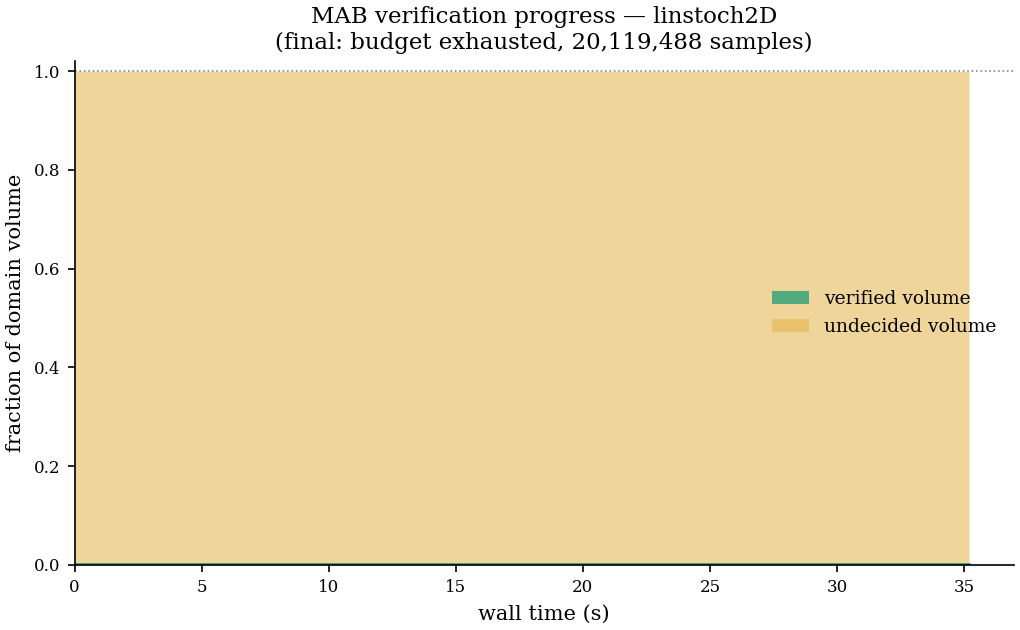
\includegraphics[width=0.49\linewidth]{Figures/mab_area.png}\hfill
% 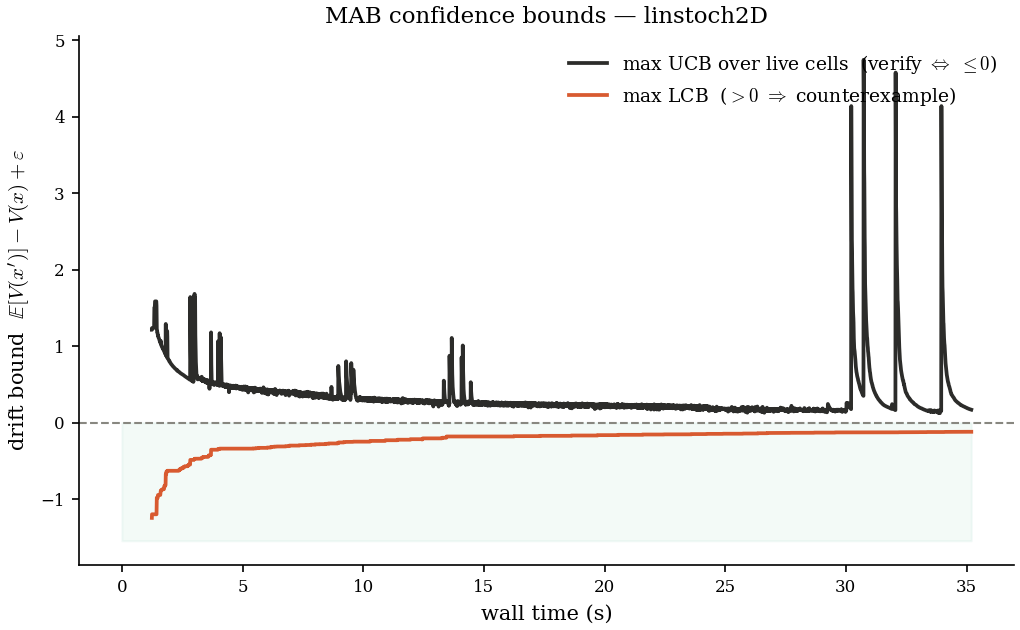
\includegraphics[width=0.49\linewidth]{Figures/mab_bounds.png}
% \caption{The MAB verifier at work on the 2D linear-stochastic certificate.
% \emph{Left:} the fraction of the domain proven safe grows over time as cells are
% retired. \emph{Right:} the global upper and lower confidence bounds on
% $\sup_{x}\drift(x)$ close towards the certification threshold; the run certifies
% once the upper bound falls to $0$. Adaptive refinement concentrates samples on
% the thin-margin frontier, so most of the domain is cleared by a few large
% cells.}
% \label{fig:mab}
% \end{figure}

% \paragraph{Monte Carlo versus MAB.}
% The two sampling verifiers share an interface and a soundness style but sit at
% opposite ends of a cost--precision trade-off. The global Monte Carlo method
% (Algorithm~\ref{alg:mc}) verifies a positive tolerance $\tau$ at cost
% $\sim\tau^{-2(d+1)}$ and can never certify $\tau=0$; a uniform Lipschitz covering
% would already reach $\tau=0$ at cost $\sim(L_{\drift}/\tau_{\mathrm{res}})^d$; and MAB
% (Algorithm~\ref{alg:mab}) attains the same zero-tolerance guarantee while
% spending that exponential cost only where the margin is thin. This progression
% --- global average, uniform cover, adaptive cover --- is precisely the ladder
% that motivates keeping spatial locality in black-box verification.


% \section{Experiments}

% Having described the three verifier families, we ask which of them can actually
% drive certificate synthesis to completion across the benchmark suite, and at
% what cost. We run each engine as the sole verifier in the CEGIS loop --- every
% counterexample is found by the verifier itself --- on the systems of
% Chapter~\ref{chap:benchmarks}, and record whether a valid certificate is reached
% together with the wall-clock and number of CEGIS rounds it takes.

% The result is a capability boundary that follows the dynamics class exactly as
% Chapter~\ref{chap:benchmarks} anticipated (Table~\ref{tab:capability}). The
% \emph{symbolic} engines are the most precise where they apply but the least
% general: Gurobi's MILP encoding is exact yet closes only up to two noise
% dimensions --- the discretisation window shuts by three
% (Figure~\ref{fig:milp_nd}) --- and Z3, though a complete decision procedure for
% the polynomial systems, returned \emph{unknown} or exhausted its budget on
% essentially every trained-network round. Neither can represent the pendulum's
% $\sin\theta$, and both abstain outright. The \emph{sampling} verifiers are the
% most general --- indifferent to the form of the dynamics and the noise --- but
% sound worst-case sampling is costly (Sections~\ref{sec:mc}--\ref{sec:mab}), and
% we were not able to drive it to a full-suite synthesis campaign within budget;
% we report it as a sound-but-expensive method rather than a benchmarked engine.

% \begin{table}[h]
% \centering
% \begin{tabular}{llcccc}
% \hline
% System & Dynamics & Z3 (SMT) & Gurobi (MILP) & LiRPA & MC/MAB \\
% \hline
% Linear (2D) & linear & exact$^\ast$ & exact ($\le$2D) & \checkmark & sound$^\dagger$ \\
% Double-well & polynomial & exact$^\ast$ & exact & \checkmark & sound$^\dagger$ \\
% Pendulum (LQR) & transcendental & abstains & abstains & \checkmark & sound$^\dagger$ \\
% \hline
% \end{tabular}
% \caption{Verifier capability across the suite. \checkmark{} = drives CEGIS to a
% valid certificate. $^\ast$ Z3 is a sound decision procedure for these systems
% but returned \emph{unknown}/timeout on essentially every trained-network round.
% $^\dagger$ the sampling verifiers are sound and general but were not run at
% full-suite scale. The bound-propagation (LiRPA) family is the only one that
% spans the suite, including the transcendental pendulum the symbolic engines
% cannot encode.}
% \label{tab:capability}
% \end{table}

% The bound-propagation (LiRPA) family is the one that spans the suite. IBP, CROWN
% and $\alpha$-CROWN each synthesise a valid certificate on the linear,
% double-well and transcendental-pendulum systems alike --- including the case the
% symbolic engines cannot even encode --- which is what identifies this family as
% the reliable default for stochastic certificate verification. The three engines
% trade per-call tightness against the number of rounds in the expected way, and
% the anytime view in Figure~\ref{fig:pendulum-anytime} makes the trade concrete:
% on a pendulum certificate, IBP's enclosure is the loosest at any compute budget,
% CROWN tightens it, and $\alpha$-CROWN's per-call slope optimisation reaches the
% tightest bound --- but at a steep price, up to $2.7$ hours to certify the
% pendulum in the verifier-only loop (the full verifier-only costs are the
% baseline rows of Table~\ref{tab:cegis-speedup}). That cost, incurred once per
% round and paid mostly on candidates that turn out to be invalid, is exactly what
% the refuter pre-screen of Chapter~\ref{chap:streamlining} removes.

% \begin{figure}[h]
% \centering
% 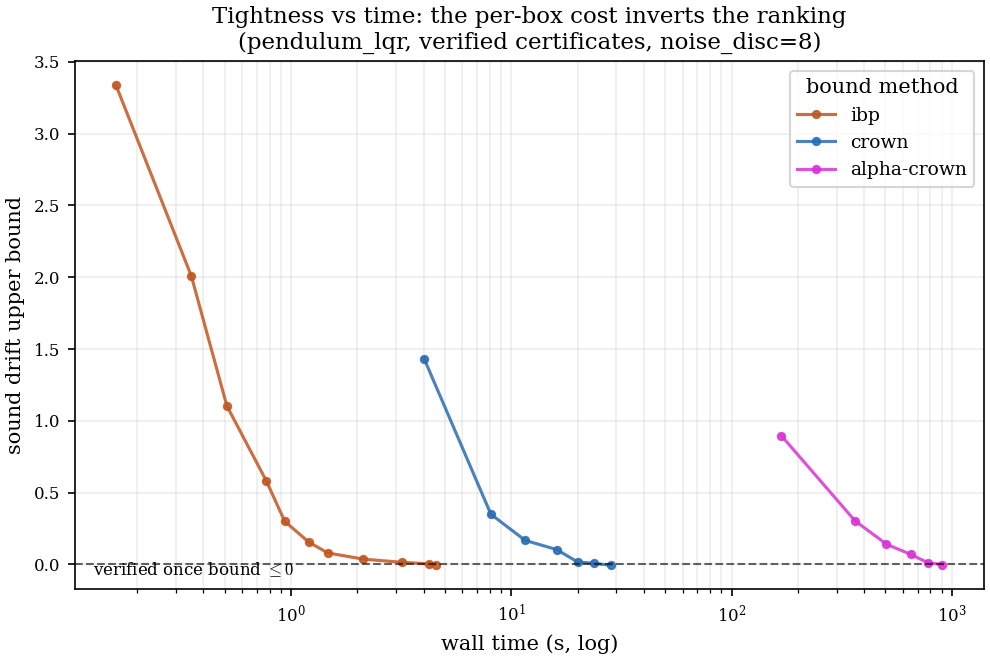
\includegraphics[width=\linewidth]{Figures/pendulum_anytime_time.png}
% \caption{Anytime tightness of the three LiRPA engines on a verified pendulum
% certificate: the certified drift bound against wall-clock as branch-and-bound
% refines. IBP is cheapest per unit compute but loosest; $\alpha$-CROWN reaches
% the tightest bound at the highest cost; CROWN sits between. All three are sound
% at every step (the bound only tightens), the property that lets them be stopped
% early inside the CEGIS loop.}
% \label{fig:pendulum-anytime}
% \end{figure}

% We now turn from the verifiers in isolation to their behaviour inside the full
% synthesis loop, where the dominant cost above --- the sound call on every
% round --- can be pre-empted by a cheap refuter; this is the subject of
% Chapter~\ref{chap:streamlining}.



\newpage



    % !TEX root = ../MasterThesis.tex
\chapter{Refutation}
\label{chap:refutation}

Refutation is the search for a counterexample that invalidates a candidate certificate. The counterexample is an explicit state in the sense of Definition~\ref{def:verification} --- one violating the condition of interest --- which we then use to guide the next round of CEGIS. Counterexamples are much easier to find than proofs of their absence, primarily because the claim changes shape: instead of establishing the condition for \emph{all} $x \in \aX$, it suffices to exhibit \emph{some} $x \in \aX$ that violates it. This lets us treat the problem as a search, which careful formulation can pose in several efficient ways. In this chapter we benchmark six black-box optimisers, testing them on standard test problems as well as real neural certificates to assess their usefulness as a dedicated subroutine in the CEGIS pipeline.


Let 
\[
x^\star = \argmax_{x \in \aX} \drift(x).
\]
From an optimisation perspective, verification checks
\[
\drift(x^\star) \leq 0,
\]
whereas any $x \in \aX$ such that
\[
\drift(x) > 0
\]
is in fact a counterexample. Whilst all the aforementioned verification methods can find these counterexamples and serve as refuters, we can also consider specialised refuters that are designed around this optimisation problem.

\section{Optimisers}

Optimisers are an attractive choice for refutation for two reasons. First, global optimisation is a mature field, so there is a large body of prior research to draw well-performing optimisers from. Second, optimisers are readily customised: the objective function, constraints, and search targets can each encode whatever information our assumptions permit, steering the search accordingly.

As this is for refutation and not for verification, strict soundness is no longer of concern, and even points that seem close to counterexamples provide insight into the margin we have certified for. This makes a Monte-Carlo approximation of the expectation good enough for our use case. For each point evaluation, we take $m$ Monte-Carlo samples of the successor state, resulting in the objective function $\tilde{\drift}(x) = \frac{1}{m} \sum_{i=1}^{m} \cert(f(x, w_i)) - \cert(x) + \varepsilon$. Occasionally this can cause spurious counterexamples, leading to bad early-termination or incorrect local maxima.


\subsection{Random Search}

Random search is the most naive method of search in which we take uniform, iid samples across $\aX$, tracking only the best evaluations and disregarding the rest. It is simple to implement, extremely fast, but completely uninformed. It effectively acts as a benchmark for counterexample quality: the larger the drift value, the larger the violation, and the better the quality of the counterexample.

\subsection{Grid Search}

Grid search is analogous to a non-adaptive MAB algorithm. We grid the domain and evaluate centres, then refine and repeat uniformly across the domain. As a result, it is often centred on the domain and takes symmetrical evaluations which can sometimes be beneficial and other times wasteful. With each iteration the number of points to evaluate grows exponentially, so its per-iteration cost climbs with the point count. Both grid search and random search are everywhere-dense in the limit of infinite resources.


\subsection{DIRECT}

DIRECT (DIviding RECTangles) \cite{Jones1993DIRECT} reframes global optimisation as a recursive partition of the search domain into hyper-rectangles, each represented by its centre. At each iteration it identifies the potentially optimal rectangles, balancing exploitation of regions with high centre values against exploration of large, under-sampled regions. Unlike traditional Lipschitz optimisation methods, DIRECT does not require a user-specified Lipschitz constant; instead, it implicitly considers all possible positive Lipschitz constants when selecting rectangles for refinement. The selected rectangles are trisected along their longest dimension(s), and the centres of the resulting subrectangles are evaluated. Because the selection rule simultaneously considers rectangles across multiple scales, DIRECT naturally balances local refinement with global exploration and rarely commits prematurely to a single basin. Aside from a small parameter $\varepsilon_{\mathrm{po}}$ used to avoid excessive refinement of the current best region, the method is effectively parameter-free. Its main computational cost lies in maintaining the growing set of rectangles and identifying the potentially optimal subset via a convex-hull computation.

\subsection{AdaLIPO}

AdaLIPO (Adaptive Lipschitz Optimisation) \cite{malherbe2017global} is a purely sample-driven Lipschitz
method. It keeps a history of evaluated points, and each iteration proposes a
large uniform pool of candidates, scoring each by the tightest upper bound its
history allows, $\min_i [\, y_i + \hat{k}\,\lVert x - x_i\rVert \,]$, and spends
its evaluation budget on the most promising ones. The Lipschitz constant
$\hat{k}$ is estimated online from the steepest slope seen so far and inflated
slightly to stay optimistic. This makes AdaLIPO a natural fit for refutation: it
exploits precisely the regularity we already assume of the drift --- its
Lipschitz continuity --- to steer samples toward the region most likely to hide
a violation, rather than searching blindly. The overhead is the pairwise
distance computation against the history, which grows with the number of
evaluations.

\subsection{Hill Climbing (HC)}

HC exploits differentiability to traverse the landscape, wherein an agent explores in the direction that the derivative is most positive. It is the counterpart to Gradient Descent, which is famously used in machine learning for minimising loss functions. In its most basic form, it is susceptible to getting stuck at local maxima, and as such we employ random restarts to encourage the agent to explore more of the state space. Because JAX provides automatic differentiation and JIT compilation, we run HC efficiently on GPU and vectorise it so that many restarts search at once. Crucially, this gradient access is an extra assumption made only by HC.

\subsection{Whale Optimisation Algorithm (WOA)}

WOA \cite{whale_oa} is a population-based metaheuristic inspired by the bubble-net hunting of
humpback whales. A population of candidate points moves each iteration by one of
three behaviours relative to the incumbent best: a shrinking \emph{encircle}, a
logarithmic \emph{spiral}, or an \emph{exploratory} step toward a random peer. A single parameter $a$ anneals
linearly over the budget, shifting the population from exploration to
exploitation. The spiral gives WOA a distinctive ability to probe around a
promising point at many radii at once, and being population-based it is
naturally parallel and resistant to being trapped by a single local optimum. It
also carries the most tuning knobs of the refuters we consider: the annealing
ceiling $a_{\max}$, the spiral tightness $b$, and the spiral/encircle mix $p$.
Crucially, WOA has a track record as a fast and flexible black-box optimiser,
performing consistently in optimiser comparisons on the Black-Box Optimisation
Benchmarking (BBOB) suite of the COCO platform \cite{hansen2021coco}.

\section{Experiments}

We study the refuters in two stages. Because they cannot certify on their own,
their value in the pipeline is as a cheap pre-screen: run up to a fixed budget
each round, falling back on the sound verifier only when no counterexample is
found --- the arrangement Chapter~\ref{chap:streamlining} evaluates
end-to-end. We first tune each refuter as a black-box optimiser on a standard benchmark suite
(Section~\ref{sec:bbob}), then turn the tuned refuters on genuine refutation
tasks (Section~\ref{sec:fauxcert}).

\subsection{Hyperparameter Tuning on BBOB}
\label{sec:bbob}

Before comparing refuters we must give each a fair chance, which means choosing
its hyperparameters well. We take five functions from the BBOB test suite, spanning
the landscape archetypes that separate search strategies: Rastrigin (f3, a
regular grid of local optima), Rosenbrock (f8, a narrow curved valley),
Schaffers~F7 (f17, irregular ripples at every radius), Schwefel (f20, best basins are far from the centre), and
Gallagher's 101-peak function (f21, a narrow needle among distractors). Each is
negated so that the refuter \emph{maximises} and the global optimum is $0$; every
function is first checked for well-formedness (Figure~\ref{fig:bbob-landscapes}).




\begin{figure}[htbp]
\centering
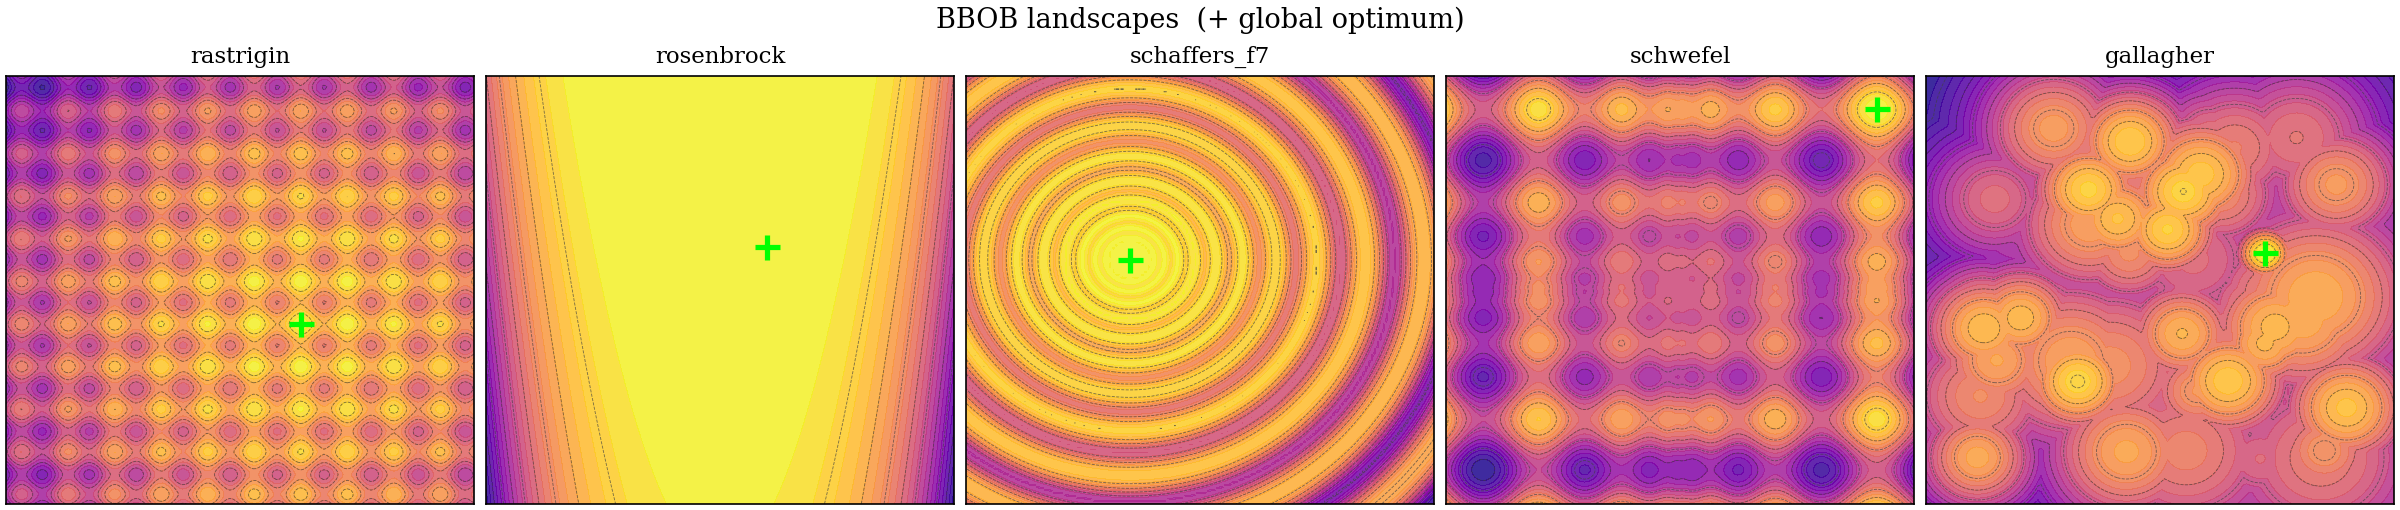
\includegraphics[width=\linewidth]{Figures/bbob_landscapes.png}
\caption{The five BBOB test functions with the
global optimum marked in green. Yellow indicates high-quality solutions and purple indicates low-quality solutions.}
\label{fig:bbob-landscapes}
\end{figure}

For each refuter we sweep its hyperparameter grid over the five functions and
three seeds at a budget of $8192$ evaluations, and score a run by its
\emph{normalised regret} $r = -\,\hat{y}^\star / \mathrm{Diam}(f) \in [0,1]$,
where $\hat{y}^\star$ is the best value found and $\mathrm{Diam}(f)$ the span of
$f$ over the domain, so that $r=0$ means the optimum was located. The best
hyperparameters for a refuter are those minimising the mean regret over
functions and seeds; Table~\ref{tab:bbob-best} reports them.

\begin{table}[htbp]
\centering
\begin{tabular}{llrr}
\hline
Refuter & Best hyperparameters & Mean regret & Time (s) \\
\hline
Whale (WOA)   & $a_{\max}=1.5,\ b=0.5,\ p=0.75$     & $5.8\times10^{-8}$ & $0.004$ \\
DIRECT        & $\varepsilon_{\mathrm{po}}=10^{-3}$ & $3.7\times10^{-5}$ & $0.148$ \\
AdaLIPO       & $\text{pool}=16,\ \alpha=0.2$       & $4.9\times10^{-4}$ & $0.686$ \\
Grid          & ---                                 & $2.3\times10^{-3}$ & $0.001$ \\
Random        & ---                                 & $5.1\times10^{-3}$ & $0.002$ \\
Hill climbing & $\text{lr}=0.5,\ \text{decay}=0.95$ & $5.7\times10^{-3}$ & $0.002$ \\
\hline
\end{tabular}
\caption{Best hyperparameters per refuter, by mean normalised regret over the
five BBOB functions and three seeds. Lower regret is
better; time is the mean wall-clock per search.}
\label{tab:bbob-best}
\end{table}

Two results stand out. First, the Lipschitz-aware and population methods
dominate the uninformed ones: whale, DIRECT and AdaLIPO reach regrets one to
five orders of magnitude below random, grid and hill climbing. Second,
accuracy need not be bought with time: whale in particular solves all five
landscapes at essentially zero regret in milliseconds, a combination that
Figure~\ref{fig:bbob-time} places on the quality--cost plane below.


Figure~\ref{fig:bbob-quality} breaks the tuned refuters down by function.
Rosenbrock's valley is easy for everyone at this budget; it is the multimodal
and deceptive functions that separate the methods. Hill climbing is competitive
only on the smooth valley and the ripples, and collapses on Schwefel (two orders
of magnitude worse than plain grid search) and Gallagher which punish pure exploitation.
 Whale and DIRECT solve every function; AdaLIPO
is a consistent middle tier. Figure~\ref{fig:refuter-patterns} shows how the refuters differ in where they
spend their evaluations on a shared landscape, from the uniform scatter of
random search to the basin-focused trajectories of the informed methods.


\begin{figure}[htbp]
\centering
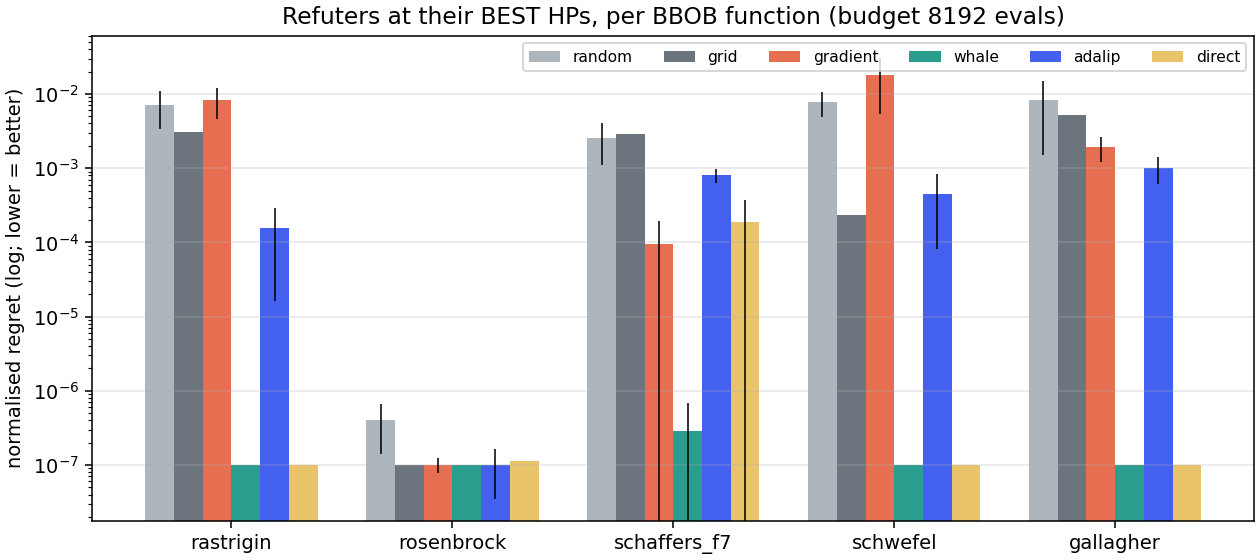
\includegraphics[width=\linewidth]{Figures/bbob_quality_per_function.png}
\caption{Normalised regret (log scale) of each refuter at its best
hyperparameters, per BBOB function. The multimodal and deceptive functions
(Schwefel, Gallagher, Rastrigin) separate the informed methods from the
uninformed ones.}
\label{fig:bbob-quality}
\end{figure}

Finally, Figure~\ref{fig:bbob-time} places quality against wall-clock cost. Two
clusters emerge: a fast-and-accurate frontier occupied by whale (millisecond
searches at essentially zero regret) and a slower, deliberate cluster (AdaLIPO
and DIRECT at tenths of a second, paying their per-iteration Lipschitz
bookkeeping for accuracy). Random, grid and hill climbing are fast but sit three
to five orders of magnitude worse on the hard functions. Whale at its tuned
configuration dominates the frontier outright, and it is these tuned
configurations that we carry into the refutation experiment that follows.

\begin{figure}[htbp]
\centering
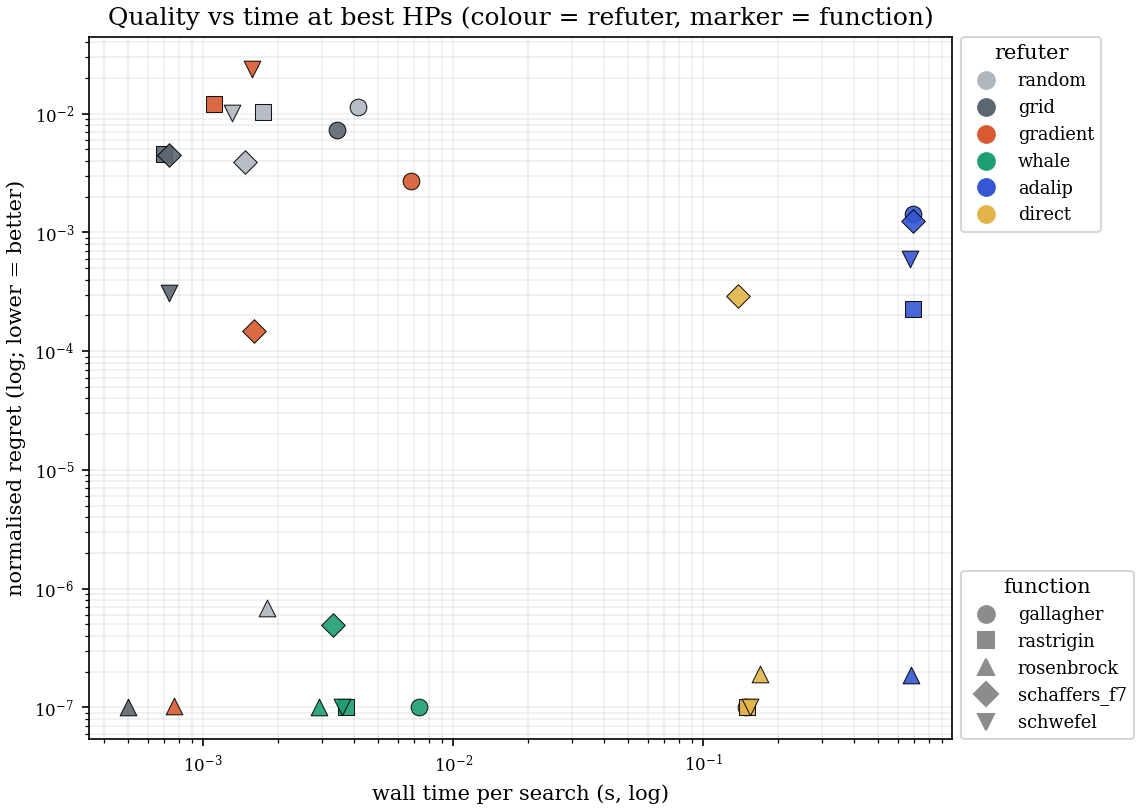
\includegraphics[width=0.8\linewidth]{Figures/bbob_quality_vs_time.png}
\caption{Quality versus wall-clock cost at the best hyperparameters (colour =
refuter, marker = function; both axes logarithmic). Whale occupies the
fast-and-accurate frontier; the Lipschitz methods trade time for accuracy;
uninformed search is fast but far worse on the hard landscapes.}
\label{fig:bbob-time}
\end{figure}

\subsection{Refuting Faux Certificates}
\label{sec:fauxcert}

The BBOB benchmark tunes and characterises the refuters as generic optimisers;
we now experiment with refuters within the context of our problem definition. Every round in
which a sound verifier (MILP or LiRPA) rejected a candidate certificate during
the verification runs of the previous chapter left behind a \emph{faux certificate}: a
trained network that looks like a valid supermartingale but violates the drift
condition somewhere, stored together with the counterexample the verifier found
and the wall-clock it took to find it. These harvested faux certificates form a
library of genuine refutation problems, drawn from the real CEGIS trajectory
rather than a synthetic benchmark.

We replay each harvested faux certificate with all six refuters at their
BBOB-tuned hyperparameters (Section~\ref{sec:bbob}), and record, against the
sound verifier that originally rejected the candidate, whether each refuter finds
a counterexample, how fast, and the \emph{quality} of the counterexample it
returns (the drift value it attains under a common high-sample estimator). Our
library holds $91$ distinct faux certificates harvested from the $\mathrm{LinSwitch}$,
$\mathrm{DoubleWell}$ and $\mathrm{Pendulum}$ verification runs, each replayed with all
six refuters, and the stochastic refuters over several random seeds.

Every refuter recovers the large majority of counterexamples far more cheaply
than the sound verifier (Figure~\ref{fig:faux-certs}, Table~\ref{tab:fauxcert}).
A single refutation costs between $1$ and $21$\,ms against the verifier's median
$0.48$\,s, for median speed-ups of $69$--$352\times$. Two axes separate the
methods. The first is \emph{reliability}: whale finds a counterexample on $99\%$
of the faux certificates across all three systems and returns the deepest ones
(median drift $0.049$)
while random, grid, AdaLIPO and hill climbing sit at $91$--$95\%$. DIRECT is the
outlier: strong on the synthetic BBOB suite, it collapses to $40\%$ here, missing
two-thirds of the linear-system certificates. The second is \emph{cost}:
the uninformed random and grid searches are the fastest per cert ($1.4$\,ms,
${\sim}350\times$) because they model nothing, whereas whale's thorough spiral
search costs more ($3.9$\,ms, ${\sim}130\times$). This is the empirical basis for the pre-screen: on the
certificates a sound verifier would reject, a cheap refuter reaches the same
verdict at a fraction of the cost, and a well-chosen one does so almost every
time.


\begin{figure}[t]
\centering
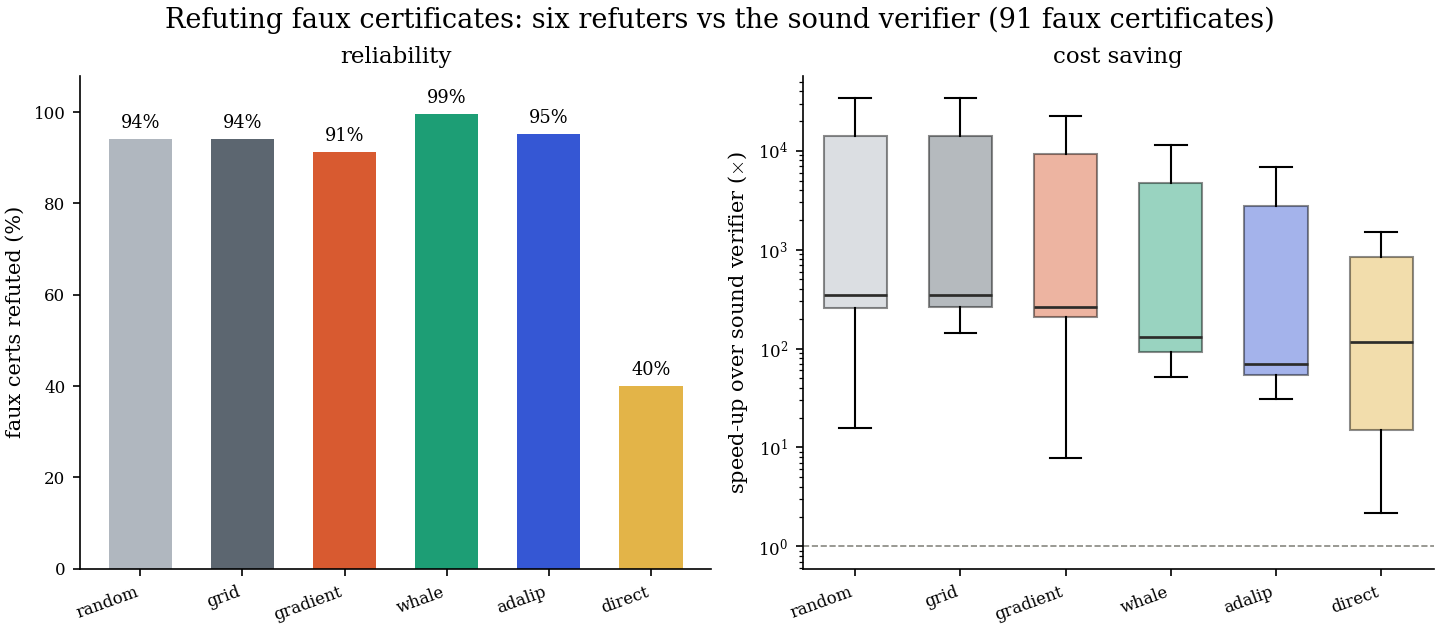
\includegraphics[width=\linewidth]{Figures/faux_certs.png}
\caption{Refuting the faux certificates a sound verifier rejected, six refuters
compared. \emph{Left:} the fraction of faux certificates each refuter refutes ---
whale is near-perfect, the other informed and uninformed methods cluster at
$91$--$95\%$, and DIRECT collapses to $40\%$. \emph{Right:} per-refuter speed-up
over the sound verifier (log): every refuter is one-to-three orders of magnitude
cheaper than a sound call, the fast uninformed searches highest.}
\label{fig:faux-certs}
\end{figure}

\begin{table}[t]
\centering
\begin{tabular}{lrrrrr}
\hline
Refuter & Success rate & Verifier (s) & Refuter (s) & Speed-up & Quality \\
\hline
Whale         & $99\%$ & $0.50$ & $0.004$ & $131\times$ & $0.049$ \\
AdaLIPO       & $95\%$ & $0.48$ & $0.007$ & $69\times$  & $0.042$ \\
Random        & $94\%$ & $0.48$ & $0.001$ & $344\times$ & $0.039$ \\
Grid          & $94\%$ & $0.48$ & $0.001$ & $352\times$ & $0.038$ \\
Hill climbing & $91\%$ & $0.48$ & $0.002$ & $262\times$ & $0.038$ \\
DIRECT        & $40\%$ & $0.48$ & $0.021$ & $116\times$ & $0.024$ \\
\hline
\end{tabular}
\caption{Faux-certificate refutation, six BBOB-tuned refuters versus the sound
verifier that rejected each candidate. Columns: the fraction of faux certificates
on which a genuine counterexample was found; \emph{median} wall-clock to a
counterexample for the verifier and the refuter, and their ratio; and median
counterexample quality (scored drift). Whale is the most reliable and returns the
deepest counterexamples; the uninformed searches are the cheapest per call;
DIRECT misses most of the linear-system certificates.}
\label{tab:fauxcert}
\end{table}


\newpage



    % !TEX root = ../MasterThesis.tex
\chapter{Streamlining CEGIS}
\label{chap:streamlining}

The preceding chapters characterised the two halves of certificate synthesis in
isolation: Chapter~\ref{chap:verification} the sound verifiers, and
Chapter~\ref{chap:refutation} the refuters as cheap counterexample search. This
chapter assembles them into the full CEGIS loop and asks: does placing a refuter in front of the sound verifier make
end-to-end certificate synthesis faster?

\section{Experimental Setup}

We run the complete CEGIS pipeline on three benchmark systems chosen to span
the difficulty spectrum of Chapter~\ref{chap:benchmarks}: the 2D $\mathrm{LinSwitch}$ (Section~\ref{sec:bench-linear}), the $\mathrm{DoubleWell}$ gradient
flow (Section~\ref{sec:bench-doublewell}), and
the LQR-controlled $\mathrm{Pendulum}$ (Section~\ref{sec:bench-pendulum-lqr}),
whose transcendental dynamics make bound propagation expensive. The fourth
benchmark, $\mathrm{LinStoch}$, is absent by necessity rather than choice:
Chapter~\ref{chap:verification} found it certifiable only by the exact MILP
route, and the LiRPA engines this campaign compares were unable to verify it,
so no verifier-only baseline exists to improve upon.

The learner trains the $\relu$ certificate architecture used throughout (two
hidden layers of eight units) to a training margin of $0.02$, and the loop
terminates when a sound verifier certifies the drift condition to
$\varepsilon = 10^{-3}$. Any counterexample found, whether by refuter or
verifier, is added to the training set and the candidate is retrained.

For our verifiers we take the three LiRPA-family engines of
Chapter~\ref{chap:verification}, the only family that certifies all three
systems. All three run inside the same branch-and-bound refinement with longest-edge region splitting. Against each engine we compare three loop configurations, which differ only in
how counterexamples are sought:

\begin{description}
\item[Verifier-only.] The baseline: the sound verifier runs every round, both
  finding counterexamples and, eventually, certifying.
\item[Random pre-screen.] Each round, random search
  (Section~\ref{sec:bbob}) hunts for a counterexample first; only when it
  finds nothing do we fall back on the sound verifier. Random is the
  uninformed extreme: essentially free, but blind.
\item[Whale pre-screen.] The same arrangement with the whale optimiser (WOA)
  at its BBOB-tuned hyperparameters (Table~\ref{tab:bbob-best}), selected because it dominated the fast-and-accurate
  frontier of the refuter benchmark.
\end{description}

Refuters run with the same budget as in Chapter~\ref{chap:refutation} ($8192$
evaluations per search, $16$ Monte-Carlo samples per point). Each
configuration is repeated over five seeds. We record the wall-clock time to a
verified certificate, the number of CEGIS rounds, the number of sound-verifier
calls, and the number of \emph{escapes} --- counterexamples the refuter
missed that the sound verifier subsequently found.

\paragraph{Compute environment.} Campaigns throughout the thesis were
dispatched as job arrays to a Slurm compute cluster; the sampling verifiers
(MC, MAB) and the three LiRPA engines benefit from GPU acceleration and ran on
GPU nodes. The MILP experiments are the exception, running locally on a
desktop CPU, as the Gurobi licence (version 13.0.1, via \texttt{gurobipy})
could not be reached from the cluster's compute nodes. All code (the
unified verifier framework, the refuters, the experiment drivers, and every
figure script) is available at
\url{https://github.com/will-bailkoski/streamlining-neural-certificates}.

\section{Results and Discussion}

%Table~\ref{tab:cegis-speedup} summarises the campaign.

\begin{table}[h]
\centering
\begin{tabular}{lllrrrrr}
\hline
Engine & System & Strategy & $n$ & Time (s) & Rounds & Calls & Speed-up \\
\hline
IBP & $\mathrm{LinSwitch}$     & verifier-only & 5 & $155.5$ & $43.8$ & $43.8$ & --- \\
    &                 & random        & 5 & $58.9$  & $18.0$ & $2.6$  & $2.64\times$ \\
    &                 & whale         & 5 & $39.8$  & $10.8$ & $1.0$  & $3.91\times$ \\
    & $\mathrm{DoubleWell}$     & verifier-only & 3 & $14.6$  & $1.3$  & $1.3$  & --- \\
    &                 & random        & 3 & $14.1$  & $1.7$  & $1.0$  & $1.03\times$ \\
    &                 & whale         & 5 & $18.4$  & $2.2$  & $1.0$  & $1.04\times$ \\
    & $\mathrm{Pendulum}$  & verifier-only & 1 & $55.0$  & $6.0$  & $6.0$  & --- \\
    &                 & random        & 2 & $33.7$  & $7.5$  & $1.0$  & $1.76\times$ \\
    &                 & whale         & 1 & $57.4$  & $10.0$ & $1.0$  & --- \\
\hline
CROWN & $\mathrm{LinSwitch}$     & verifier-only & 5 & $44.6$  & $11.8$ & $11.8$ & --- \\
      &                 & random        & 5 & $52.2$  & $15.4$ & $2.0$  & $0.85\times$ \\
      &                 & whale         & 5 & $38.5$  & $10.8$ & $1.0$  & $1.16\times$ \\
      & $\mathrm{DoubleWell}$     & verifier-only & 3 & $41.7$  & $1.7$  & $1.7$  & --- \\
      &                 & random        & 5 & $31.3$  & $2.2$  & $1.0$  & $1.48\times$ \\
      &                 & whale         & 5 & $32.0$  & $2.2$  & $1.0$  & $1.51\times$ \\
      & $\mathrm{Pendulum}$  & verifier-only & 3 & $203.1$ & $7.0$  & $7.0$  & --- \\
      &                 & random        & 4 & $57.8$  & $6.8$  & $1.0$  & $2.74\times$ \\
      &                 & whale         & 4 & $66.8$  & $8.5$  & $1.0$  & $3.19\times$ \\
\hline
$\alpha$-CROWN & $\mathrm{LinSwitch}$  & verifier-only & 5 & $935.0$  & $69.2$ & $69.2$ & --- \\
               &              & random        & 5 & $91.8$   & $15.4$ & $2.0$  & $10.19\times$ \\
               &              & whale         & 5 & $59.6$   & $10.8$ & $1.0$  & $15.70\times$ \\
               & $\mathrm{DoubleWell}$  & \multicolumn{6}{c}{\emph{(did not complete)}} \\
               & $\mathrm{Pendulum}$ & verifier-only & 4 & $9559.4$ & $8.0$  & $8.0$  & --- \\
               &              & random        & 4 & $1363.0$ & $6.8$  & $1.0$  & $5.97\times$ \\
               &              & whale         & 4 & $1331.5$ & $8.8$  & $1.0$  & $6.81\times$ \\
\hline
\end{tabular}
\caption{End-to-end CEGIS performance per engine, system and counterexample
strategy: mean wall-clock time, CEGIS rounds and sound-verifier calls over the
$n$ completed seeds. Speed-ups are ratios of seed-matched means against the
verifier-only baseline. $39$ of the $135$ configured arms did not complete
(hence the uneven $n$); in particular the $\alpha$-CROWN $\mathrm{DoubleWell}$ arms are
absent, and the IBP $\mathrm{Pendulum}$ cells are single-seed and admit no matched
comparison. The IBP $\mathrm{LinSwitch}$ baseline mean is inflated by a single runaway seed
(see text).}
\label{tab:cegis-speedup}
\end{table}

\textbf{Wall time improvements.} Stripping out the repeated sound calls changes
what a run spends its time on, not merely how long it takes. Averaged over the
three engines, sound verification is the largest single cost of a verifier-only
run --- a mean $62\%$ of its wall time, against $38\%$ for training and loop
overhead. A refuter pre-screen inverts this balance: verification falls to a mean
$47\%$ of wall time while training-and-overhead rises to $48\%$ and becomes the
dominant term, and the refuter's own search accounts for only about $5\%$ --- a
second or two per run at this budget. Once the refuter absorbs the counterexample
search, in other words, CEGIS is no longer verification-bound but
\emph{training}-bound.

How cleanly this holds depends on the engine's per-call cost. Under CROWN it is a
clean inversion --- verification drops from $57\%$ of a baseline run to $46\%$ and
retraining overtakes it at $49\%$. Under IBP the loop is training-bound from the
start: IBP's calls are so cheap that training is already $58\%$ of the
verifier-only run and merely edges up to $62\%$ with a refuter, so here the
refuter's payoff is rounds saved rather than call-time skipped. At the far end,
$\alpha$-CROWN's single sound call is costly enough that verification stays
dominant even after the repeats are gone --- still $68\%$ of a refuter run on
average, and $98\%$ on $\mathrm{Pendulum}$. Verification ceases to dominate exactly when a single sound
call is cheap relative to training, which is the regime the pre-screen is built to
create.

\textbf{Difficulty scaling.} On $\mathrm{Pendulum}$ under CROWN, where a single sound verification
costs $22$--$34$\,s, the refuter arms synthesise a certificate $2.7$--$3.2$
times faster than the baseline; on $\mathrm{LinSwitch}$ under $\alpha$-CROWN,
whose slope optimisation raises the per-call cost to $9$--$18$\,s, the speed-up
reaches $10.2\times$ for random and $15.7\times$ for whale --- the largest in
the campaign, because the verifier-only baseline there spirals to $69$ rounds
($935$\,s) that the refuter collapses to about $11$. Conversely, on the same
$\mathrm{LinSwitch}$ under plain CROWN a call costs well under a second, so there is
nothing worth saving: random search actually \emph{slows the loop down}
($0.85\times$), and whale's modest $1.16\times$ gain comes from needing fewer
rounds rather than from cheaper rounds. $\mathrm{DoubleWell}$ sits in between: most
seeds certify in one or two rounds, leaving little verification to skip. The
extreme case is $\mathrm{Pendulum}$ under $\alpha$-CROWN, where a single sound call
costs some $20$ \emph{minutes}: the verifier-only baseline makes six to eleven
of them --- one-and-a-half to three-and-a-half \emph{hours} per run --- while
each refuter arm makes exactly one and completes in around $22$ minutes, a
$6.8\times$ speed-up. At this price the pre-screen is the difference between an
overnight campaign and a coffee break.

The mechanism is visible in the calls column of Table~\ref{tab:cegis-speedup}.
The baseline pays one sound verification per round (up to seventy on the
$\alpha$-CROWN $\mathrm{LinSwitch}$), whereas the refuter arms finish with a handful
of sound calls at most, and whale with exactly one: the final, unavoidable
certification call. The refuters' own cost is negligible at this budget, a
second or two per run in total. The saving is therefore the per-call
verification cost multiplied by the rounds avoided, which is why the speed-up
tracks the engine and system so closely: skipping a dozen sub-second calls buys
nothing, while skipping several twenty-minute calls buys hours.

\textbf{Counterexample leakage.} In $12$ of $33$
completed random runs the refuter declared a candidate clean that the sound
verifier then refuted --- $18$ escaped counterexamples in all, each costing an
extra expensive verification round. Whale escaped nothing: in all $34$ of its
completed runs the first certificate it passed to the verifier was accepted,
so every whale run ended with exactly one sound call. Counterexample
\emph{quality} matters too, not just detection: on $\mathrm{LinSwitch}$ random
needed $15.4$ rounds on average against the baseline's $11.8$ while whale needed $10.8$,
matching the verifier-quality counterexamples of the baseline.

A reassuring consistency check: whale's round counts are identical, seed for
seed, under all three engines ($\mathrm{LinSwitch}$: $11,8,9,10,16$) --- because it
never lets the sound verifier find a counterexample, its loop trajectory
decouples from the verification engine entirely, whose only remaining role is
to price the final call. Random's trajectories match across CROWN and
$\alpha$-CROWN ($15.4$ rounds) but drift under IBP ($18.0$): each escape hands
control back to the engine, and a loose engine returns different, weaker
counterexamples.

\textbf{Engine choice.} Per-call costs span more than three orders of magnitude across the
campaign: IBP from $0.2$\,s ($\mathrm{LinSwitch}$) to $11$\,s ($\mathrm{DoubleWell}$), CROWN from
$0.5$\,s to $34$\,s, and $\alpha$-CROWN from $9$\,s to some $1200$\,s on
$\mathrm{Pendulum}$. Reaching for the cheapest engine instead of a refuter is a false
economy, however. IBP's loose enclosures produce weak counterexamples, and on
one $\mathrm{LinSwitch}$ seed the verifier-only loop spiralled: $179$ rounds, $633$\,s,
and a final certificate with a Lipschitz constant of $58$ against the $3$--$7$
typical of the other engines. Notably, the pre-screen \emph{rescues} this
failure --- fed on refuter counterexamples instead of IBP's own, the same seed
certifies in $16$ rounds ($56$\,s, $11\times$ faster) under whale. Here the
gain is not skipped call-time (IBP's calls are nearly free) but avoided rounds:
the refuter pays off through two distinct channels, skipping expensive sound
calls \emph{and} supplying better counterexamples than a loose verifier can
produce. A tight engine guarded by a refuter pre-screen obtains tight bounds
while paying the expensive call only once.

\section{Conclusions}

Sound verification is the price of a guarantee, but it need not be paid every
round. A cheap refuter in front of the verifier reduces CEGIS to a sequence
of fast search-and-retrain rounds followed by a single certification call,
and the resulting speed-up scales with how expensive that call is: from
nothing when verification is sub-second, to $3$--$4\times$ when calls cost
tens of seconds, to $15.7\times$ on the $\alpha$-CROWN $\mathrm{LinSwitch}$ runaway and a
practical necessity on the $\alpha$-CROWN $\mathrm{Pendulum}$, where $20$-minute sound
calls turn a multi-hour verifier-only run into a $22$-minute one. The benefit
flows through two channels: skipping
expensive sound calls, and feeding the learner better counterexamples than a
loose verifier can produce --- the latter rescuing IBP from a $179$-round
runaway. The quality of the refuter governs how much of this is realised: an
uninformed search leaks counterexamples back to the verifier and pads the
loop with uninformative rounds, while the tuned whale optimiser matched the
verifier's own counterexample quality at a fraction of its cost, never
leaked, and made the loop's trajectory independent of the engine beneath it.
The practical recipe for streamlining CEGIS is therefore to pair the tightest
verifier one can afford with a well-tuned refuter pre-screen, rather than to
economise on the verifier itself.

\section{Future Work}

The field offers no shortage of hard problems; we highlight the directions that
are opened directly by a finding of this thesis.

\paragraph{Nonlinear drift-Lipschitz bounds.} Both Lipschitz contributions of
Chapter~\ref{sec:lipschitz} lean on the linearity that keeps the drift
piecewise linear, but the principle behind them --- bound the object the
verifier consumes, rather than composing bounds on its factors --- does not.
Running bound propagation over the composed graph $\cert \circ f - \cert$
would extend the tight drift constant, and its per-axis refinement, to
nonlinear dynamics.

\paragraph{Closing the $\mathrm{LinStoch}$ gap.} The capability boundary of
Chapter~\ref{chap:verification} leaves exactly one system uncertified by any
relaxation-based engine: $\mathrm{LinStoch}$, whose noise-floor equilibrium
leaves the relaxations too little margin to work with. Diagnosing that
interaction (for instance by decoupling the equilibrium the learner trains
against from the one the verifier certifies) is a self-contained problem
whose solution would make the bound-propagation family genuinely
suite-spanning.

\paragraph{Rescuing sound sampling.} The sampling verifiers of
Chapter~\ref{chap:verification} failed on loose inputs rather than broken
theory: termination stalled on the magnitude of the Lipschitz and statistical
radii. The anisotropic per-axis constants of Chapter~\ref{sec:lipschitz} plug
directly into the bandit's splitting rule, and variance-adaptive concentration
bounds attack the statistical term. Success here would be significant, as it
would deliver a sound verifier for genuinely black-box dynamics, which no
other family can offer.

\paragraph{Refuter--verifier co-design.} The pre-screen of this chapter treats
the refuter and the verifier as strangers who share only a training set. A
natural next step is to let the refuter's near-violations warm-start the
verifier's branch-and-bound, seeding splits where the margin is thinnest,
and to make the fall-back policy adaptive, spending refuter budget in
proportion to how often it has recently let a counterexample escape.

\paragraph{Broader specifications and certificate classes.} We claimed in
Chapter~\ref{sec:preliminaries} that our methods extend to safety and
reach-avoid specifications without essential modification; that claim deserves
an experiment. Likewise, this thesis used piecewise-linear certificates
throughout: smooth activations such as $\tanh$ remove the symbolic engines
from play but remain within reach of bound propagation, and
Lipschitz-constrained architectures interact directly with the margin budget
\eqref{eq:budget}. Both would re-draw the capability boundary this thesis
mapped.


\newpage


    
    \listoffigures
    \newpage
    \listoftables
    
    % appendices come here
    %\bibliographystyle{naturemag}
    %% USE DOIs in your references whenever possible
    \bibliographystyle{plainurl}
    \bibliography{bibliography}
    
    \appendix


\chapter{2D Benchmark Phase Portraits}
\label{app:benchmark-portraits}

Phase portraits of the four 2D benchmark systems introduced in
Chapter~\ref{chap:benchmarks}. In each panel the faint streamlines trace the
\emph{expected} one-step drift $\expe_w[f(x,w)] - x$ --- estimated by Monte-Carlo,
so they are valid for additive, switched and state-dependent noise alike --- while
the coloured curves are stochastic sample trajectories rolled out from random
starts inside the domain (dark to light with elapsed time). The domain boundary is
drawn in black and the equilibrium region as a red dashed circle.

\begin{figure}[htbp]
\centering
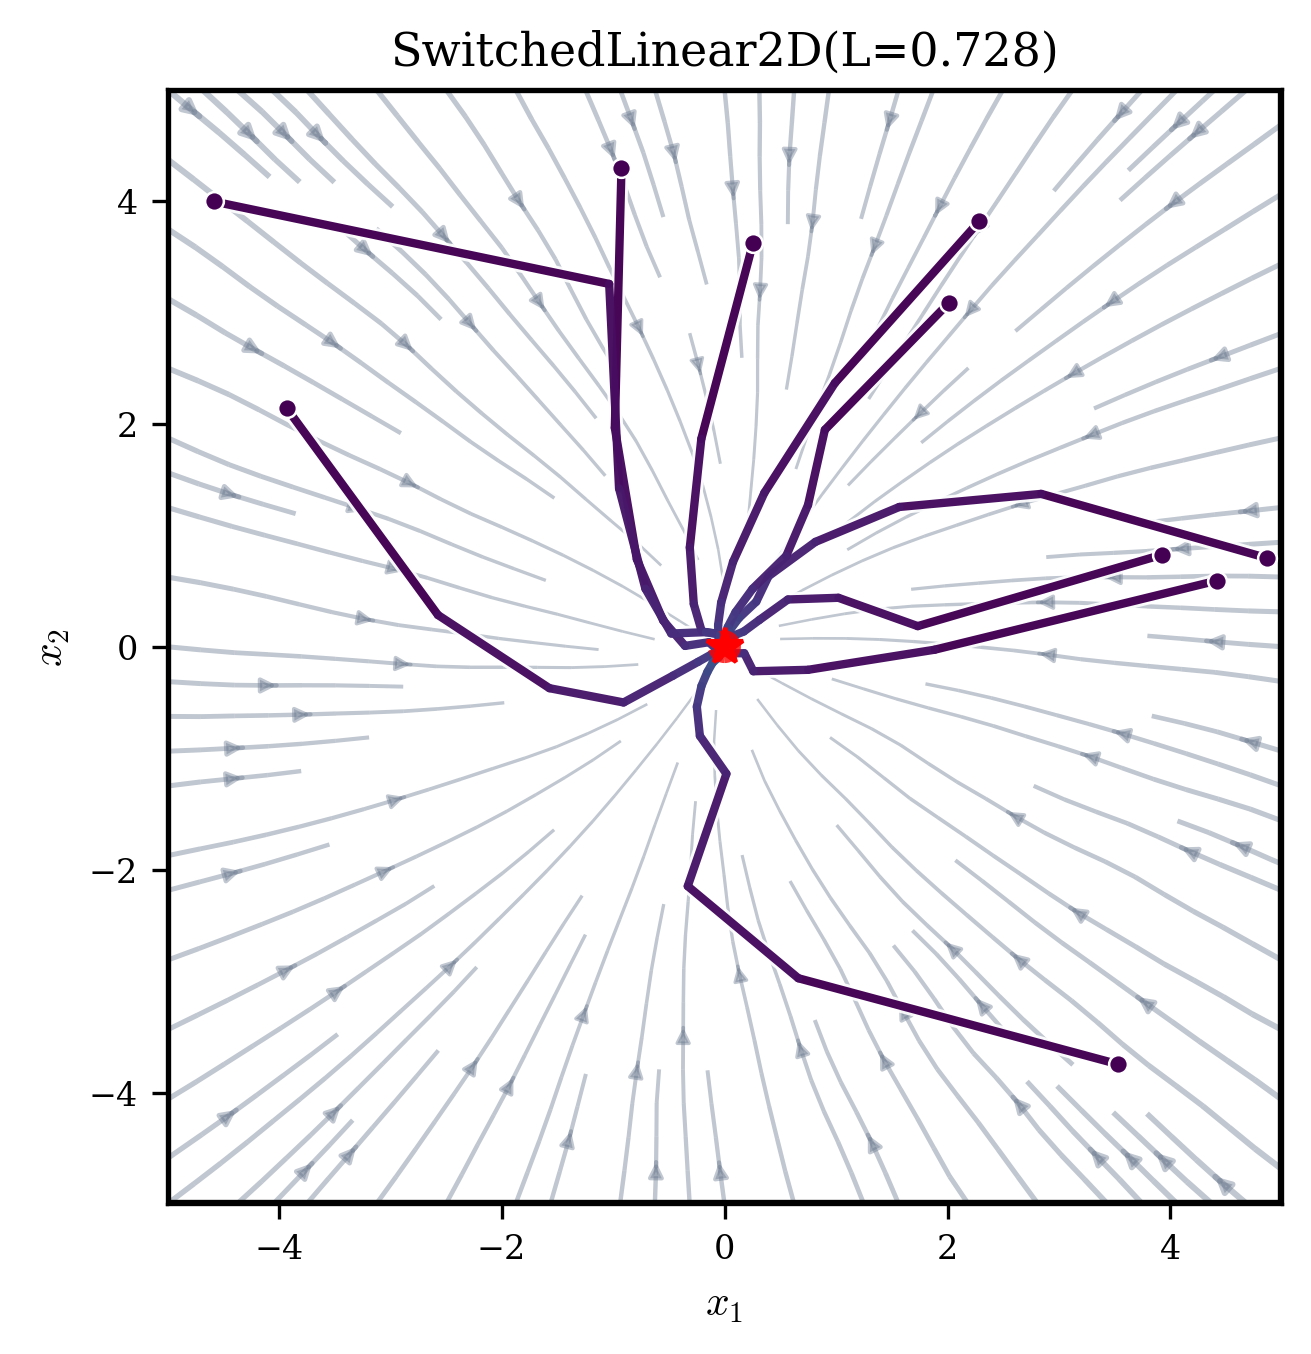
\includegraphics[width=0.55\linewidth]{Figures/linear2D_phase.png}
\caption{$\mathrm{LinSwitch}$ (Section~\ref{sec:bench-switched}): the randomly
switched linear system. Both switching modes are $L_1$-contractive, so every
trajectory collapses to the origin irrespective of the switching sequence.}
\label{fig:phase-linswitch}
\end{figure}

\begin{figure}[htbp]
\centering
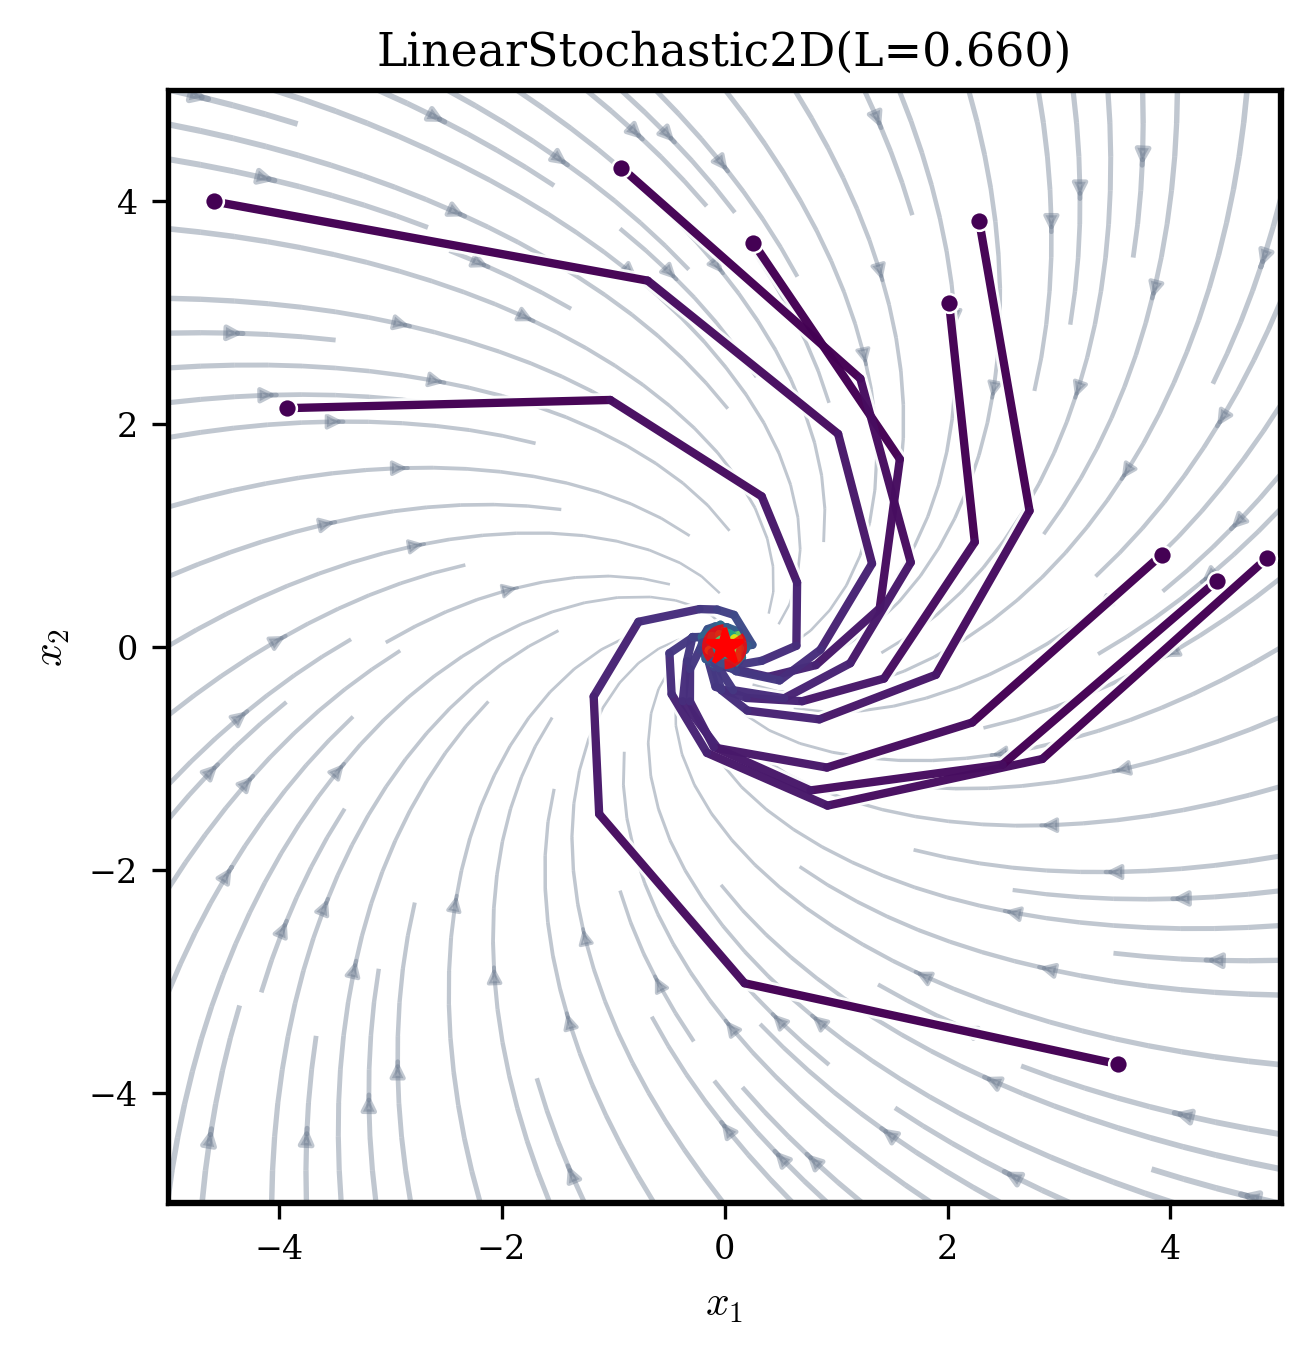
\includegraphics[width=0.55\linewidth]{Figures/linstoch2D_phase.png}
\caption{$\mathrm{LinStoch}$ (Section~\ref{sec:bench-linstoch}): the additive-noise
linear system. The Schur-stable drift spirals trajectories inward until the noise
floor halts them in a neighbourhood of the origin --- the equilibrium ball the
certificate must enclose.}
\label{fig:phase-linstoch}
\end{figure}

\begin{figure}[htbp]
\centering
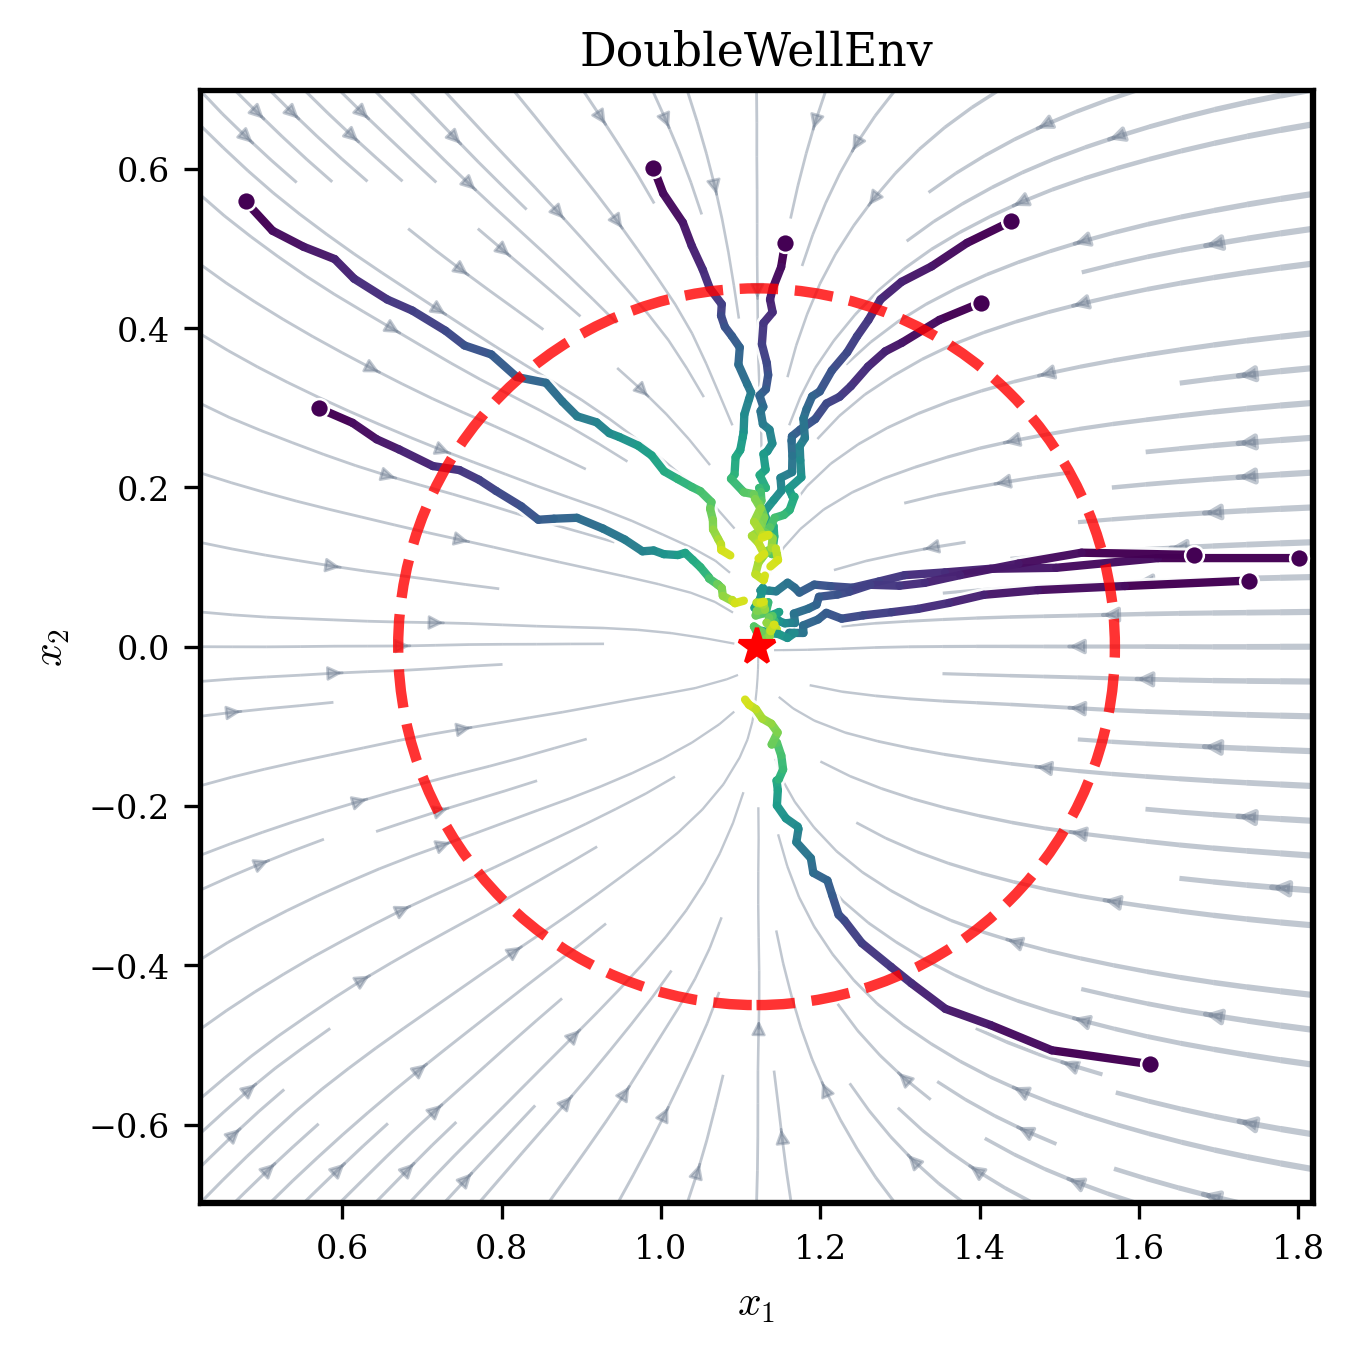
\includegraphics[width=0.55\linewidth]{Figures/doublewell_phase.png}
\caption{$\mathrm{DoubleWell}$ (Section~\ref{sec:bench-doublewell}): the tilted
stochastic gradient flow, shown zoomed onto its true attractor at $\approx(1,0)$
--- the off-origin equilibrium that sets this system apart from the others.}
\label{fig:phase-doublewell}
\end{figure}

\begin{figure}[htbp]
\centering
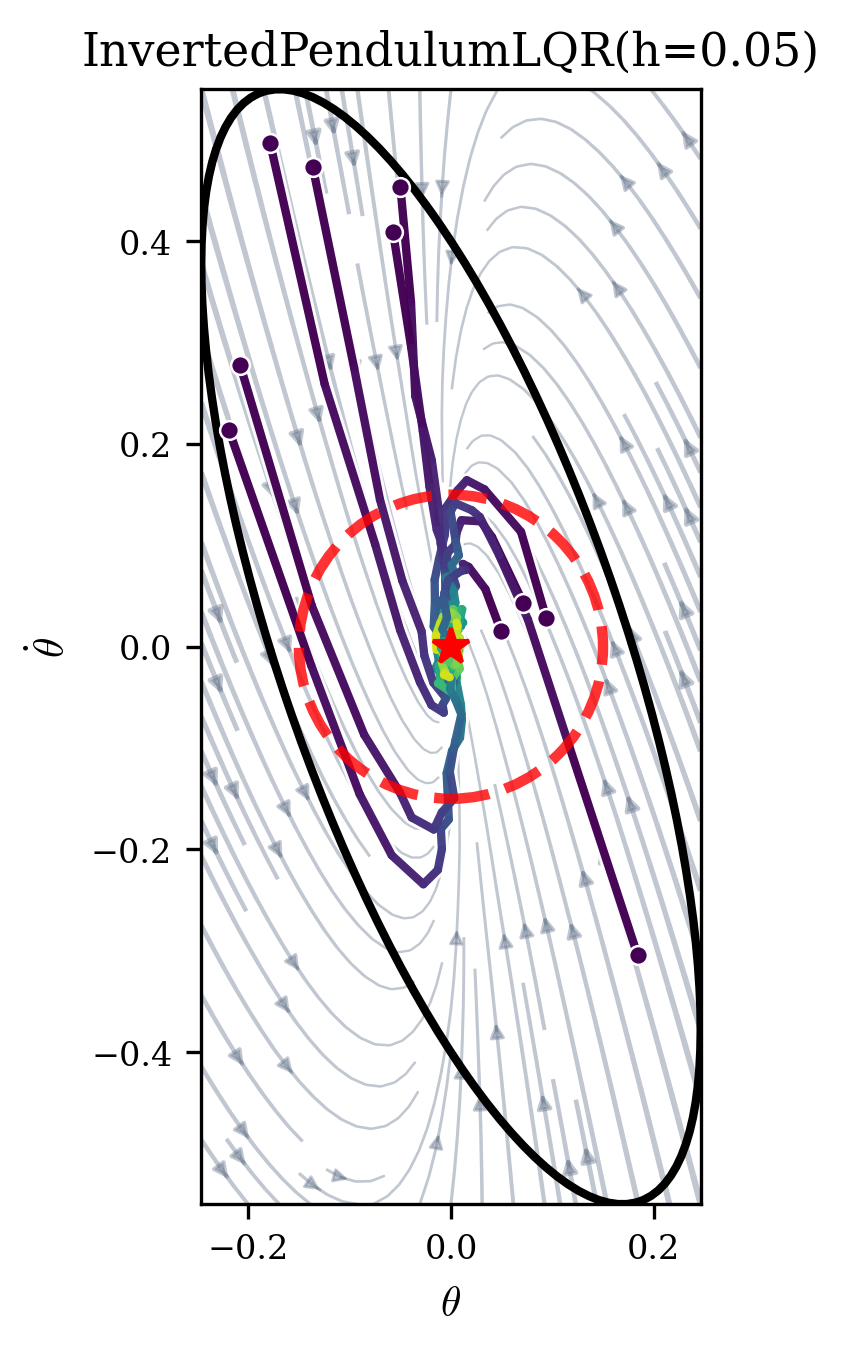
\includegraphics[width=0.36\linewidth]{Figures/pendulum_lqr_phase.png}
\caption{$\mathrm{Pendulum}$ (Section~\ref{sec:bench-pendulum-lqr}): the
LQR-controlled inverted pendulum in the $(\theta,\dot\theta)$ plane. The closed
loop is Schur-stable but non-normal, so the forward-invariant domain is the
Lyapunov sublevel ellipsoid (black) rather than a box; trajectories spiral into
the upright equilibrium.}
\label{fig:phase-pendulum}
\end{figure}


\chapter{Examples of Refuter Search Patterns}

This appendix supplements the refuter benchmark of Section~\ref{sec:bbob} with a
qualitative view of how each method spends its evaluation budget.
Figure~\ref{fig:refuter-patterns} overlays the sampled points of every refuter on
the five BBOB landscapes, at the same fixed budget, making visible the difference
between uninformed search and the informed methods that concentrate around
promising basins.

\begin{figure}[htbp]
\centering
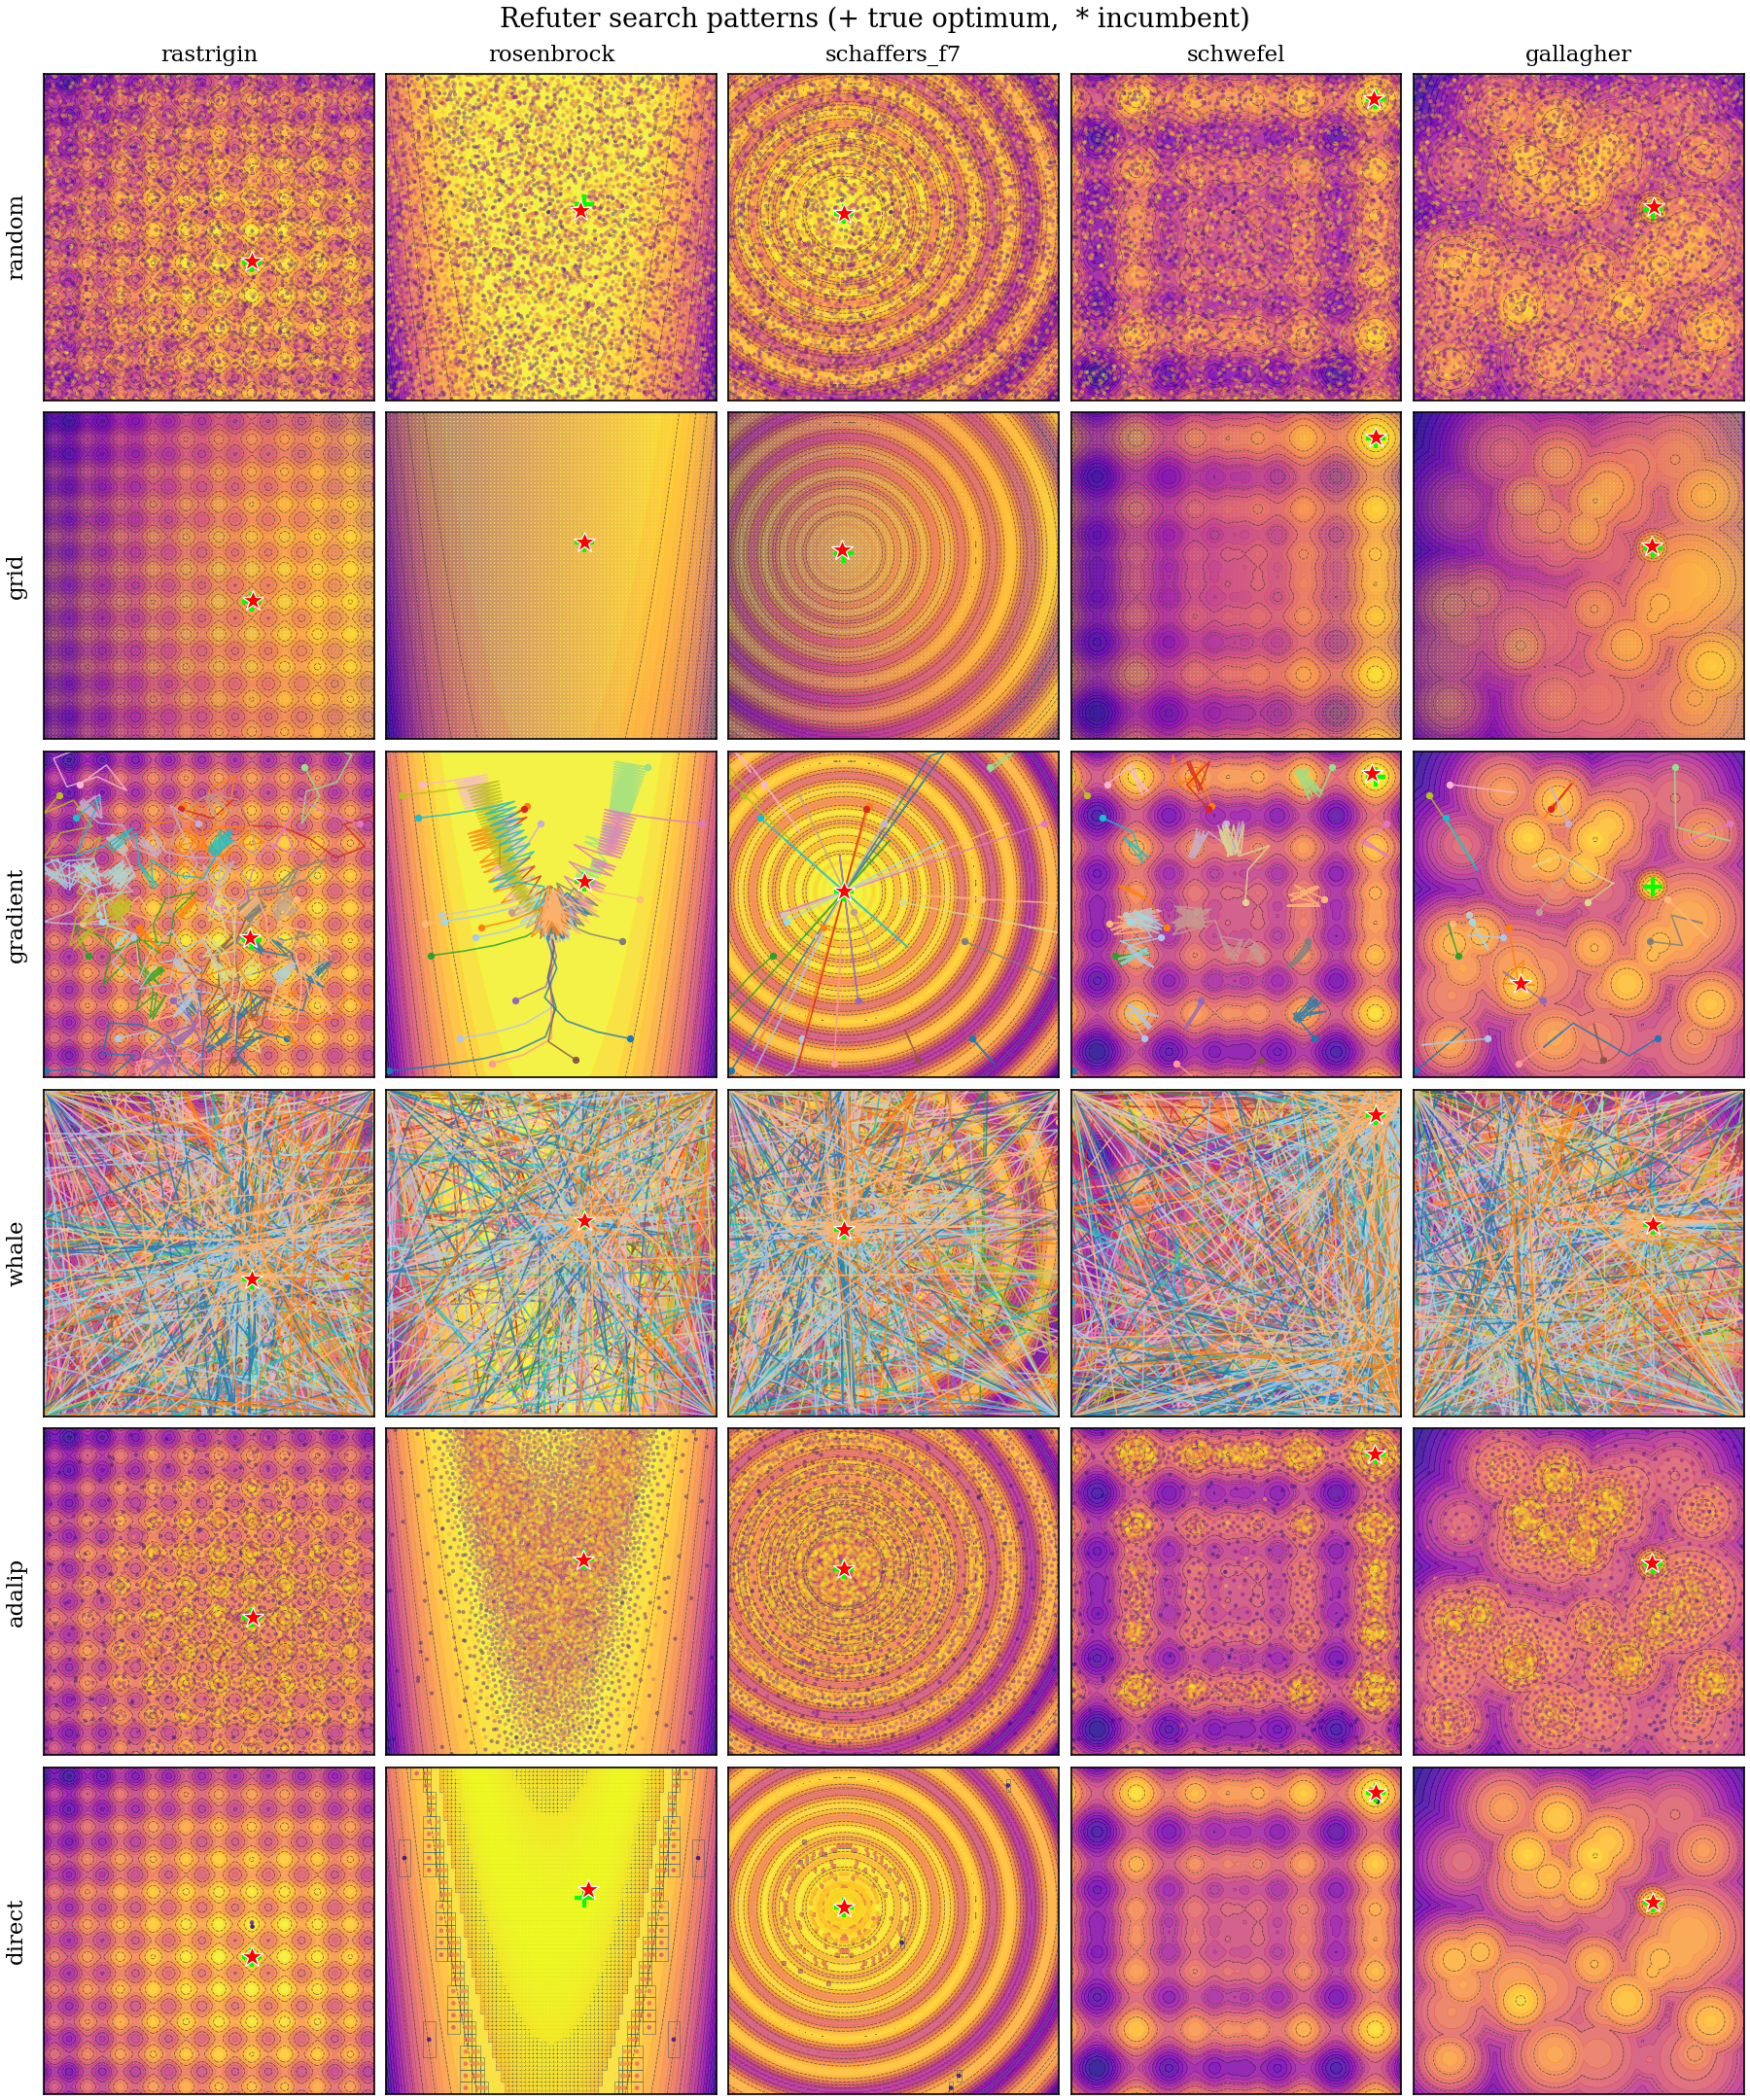
\includegraphics[width=\linewidth]{Figures/refuter_search_patterns.png}
\caption{Evaluation patterns of each refuter over a BBOB landscape at a fixed
budget. Uninformed methods (random, grid) spread evaluations evenly; the
Lipschitz-aware and population methods (DIRECT, AdaLIPO, whale) concentrate
around promising basins, which is what lets them locate deceptive optima the
uninformed methods miss.}
\label{fig:refuter-patterns}
\end{figure}

\newpage

%\fi

\end{document}